\documentclass[a4paper,twoside,openany,titlepage]{book}

\title{Appunti del corso di Fisica Cosmica 1, professor G. Lodato, anno accademico 2018-2019}
\author{Giulio Bettoni}


%COMPRESSIONE
%%\pdfcompresslevel=9
%\pdfobjcompresslevel=2

%IMPAGINAZIONE E SCRITTURA
\usepackage{makeidx}
\usepackage[italian]{babel}
\usepackage[utf8]{inputenc}
\usepackage{lmodern}
\usepackage[T1]{fontenc}
\usepackage{fancyhdr}
%\usepackage[marginparwidth=1.5cm, marginparsep=1.5cm]{geometry}				%permette di usare tutta la pagina
\usepackage[a-1b]{pdfx}
\usepackage[pdfa]{hyperref}				%permete di effettuare collegamenti tra i documenti citati 
\usepackage{verbatim}				%permette di commentare più righe
\usepackage{lipsum} 				%generatore di testo
\usepackage{marginnote}
\usepackage{MyPackage}			%Pacchetto con i comandi che ho definito io

%BIBLIOGRAFIA
\usepackage[autostyle,italian=guillemets]{csquotes}
\usepackage{natbib}
\bibliographystyle{apa-good}

%IMMAGINI GRAFICI TABELLE
\usepackage{graphicx}
\usepackage{subfig}
\usepackage{booktabs}
\usepackage[labelfont=bf]{caption}
%\usepackage[x11names]{xcolor}
\usepackage{multirow}
%\usepackage{tabularx}


%MATEMATICA
\usepackage{amsmath}
\usepackage{gensymb}
\usepackage{fixmath}
\usepackage{siunitx}
\usepackage{bigints}
\DeclareMathOperator{\sinc}{sinc}


%COMANDI
\newcommand{\cors}[1]{\textit{#1}}	%Ho creato un nuovo comando per mettere in corsivo le parole
\newcommand{\shish}{\mathrm}



\includeonly{%
Interazione_radiazione_materia,
Fluidodinamica
}

%\fancyhf{} % meglio precisare!
%\fancyhead[LE]{\slshape \leftmark}
%\fancyhead[RO]{\slshape \rightmark}
%\fancyfoot[C]{\thepage}
%\renewcommand{\headrulewidth}{0.4pt}
%\renewcommand{\footrulewidth}{0pt}


\pagestyle{fancy}
\renewcommand{\chaptermark}[1]{\markboth{}{}} %toglie il nome del capitolo dallo stile di pagina fancy
\renewcommand{\headrulewidth}{0.4pt}
%\renewcommand{\headsep}{18pt}


%CORPO DEL DOCUMENTO
\begin{document}
\date{}
\maketitle
%\pagenumbering{gobble}
%\newpage
\newpage
\pagenumbering{arabic}
\frontmatter					% è la parte introdutiva del documento, numerata in numeri romani
\tableofcontents				%compone l'indice
\mainmatter	
\chapter{Interazione radiazione-materia}
	\label{chap:InterazioneRadiazioneMateria}
La quasi totalità dell'informazione di oggetti astrofisci è trasmessa tramite la radiazione elettromagnetica, usata come diagnostica della struttura fisica dell'oggetto emittente, spesso tutt'altro che banale. Un esempio è la nebulosa del granchio in figura \ref{fig:Crab}, in cui un'analisi dello spettro della parte bluastra rivela che tale radiazione sia emissione di sincrotrone, forendo utili informaizoni circa la struttura della nebulosa (campi magnetici, presenza di plasma...). La radiazione emessa dagli oggetti celesti viene di norma alterata in modo più o meno significativo nel tragitto fino a noi da materiali interposti come le polveri del \textit{mezzo interstellare} (ISM), o nebulose. A causa della dipendenza dell'assorbimento dalla lunghezza d'onda della radiazione, è possibilie caratterizzare questi materiali interposti, determinandone la composizione chimica, la densità e le dimensioni dei grani di polveri. 
Un importante fenomeno dovuto all'assorbimento consiste nell'osservazione di un gran numero di righe spettrali Lymann $\alpha$ a lunghezze d'onda maggiori di quella attesa. Ciò è dovuto agli assorbimenti della radiazione proveniente da sorgenti a grandi distanze in cui il redshift (associato all'espansione dell'universo) ha valori diversi, e quindi lo spostamento Doppler della riga Lymann $\alpha$ dipende dalla distanza a cui è avvenuto l'assorbimento. Ciò provoca una sequenza di sfasamenti Doppler della Lymann $\alpha$, nota come \textit{foresta di Lymann $\alpha$}.
\begin{figure}[b!]
\begin{center}
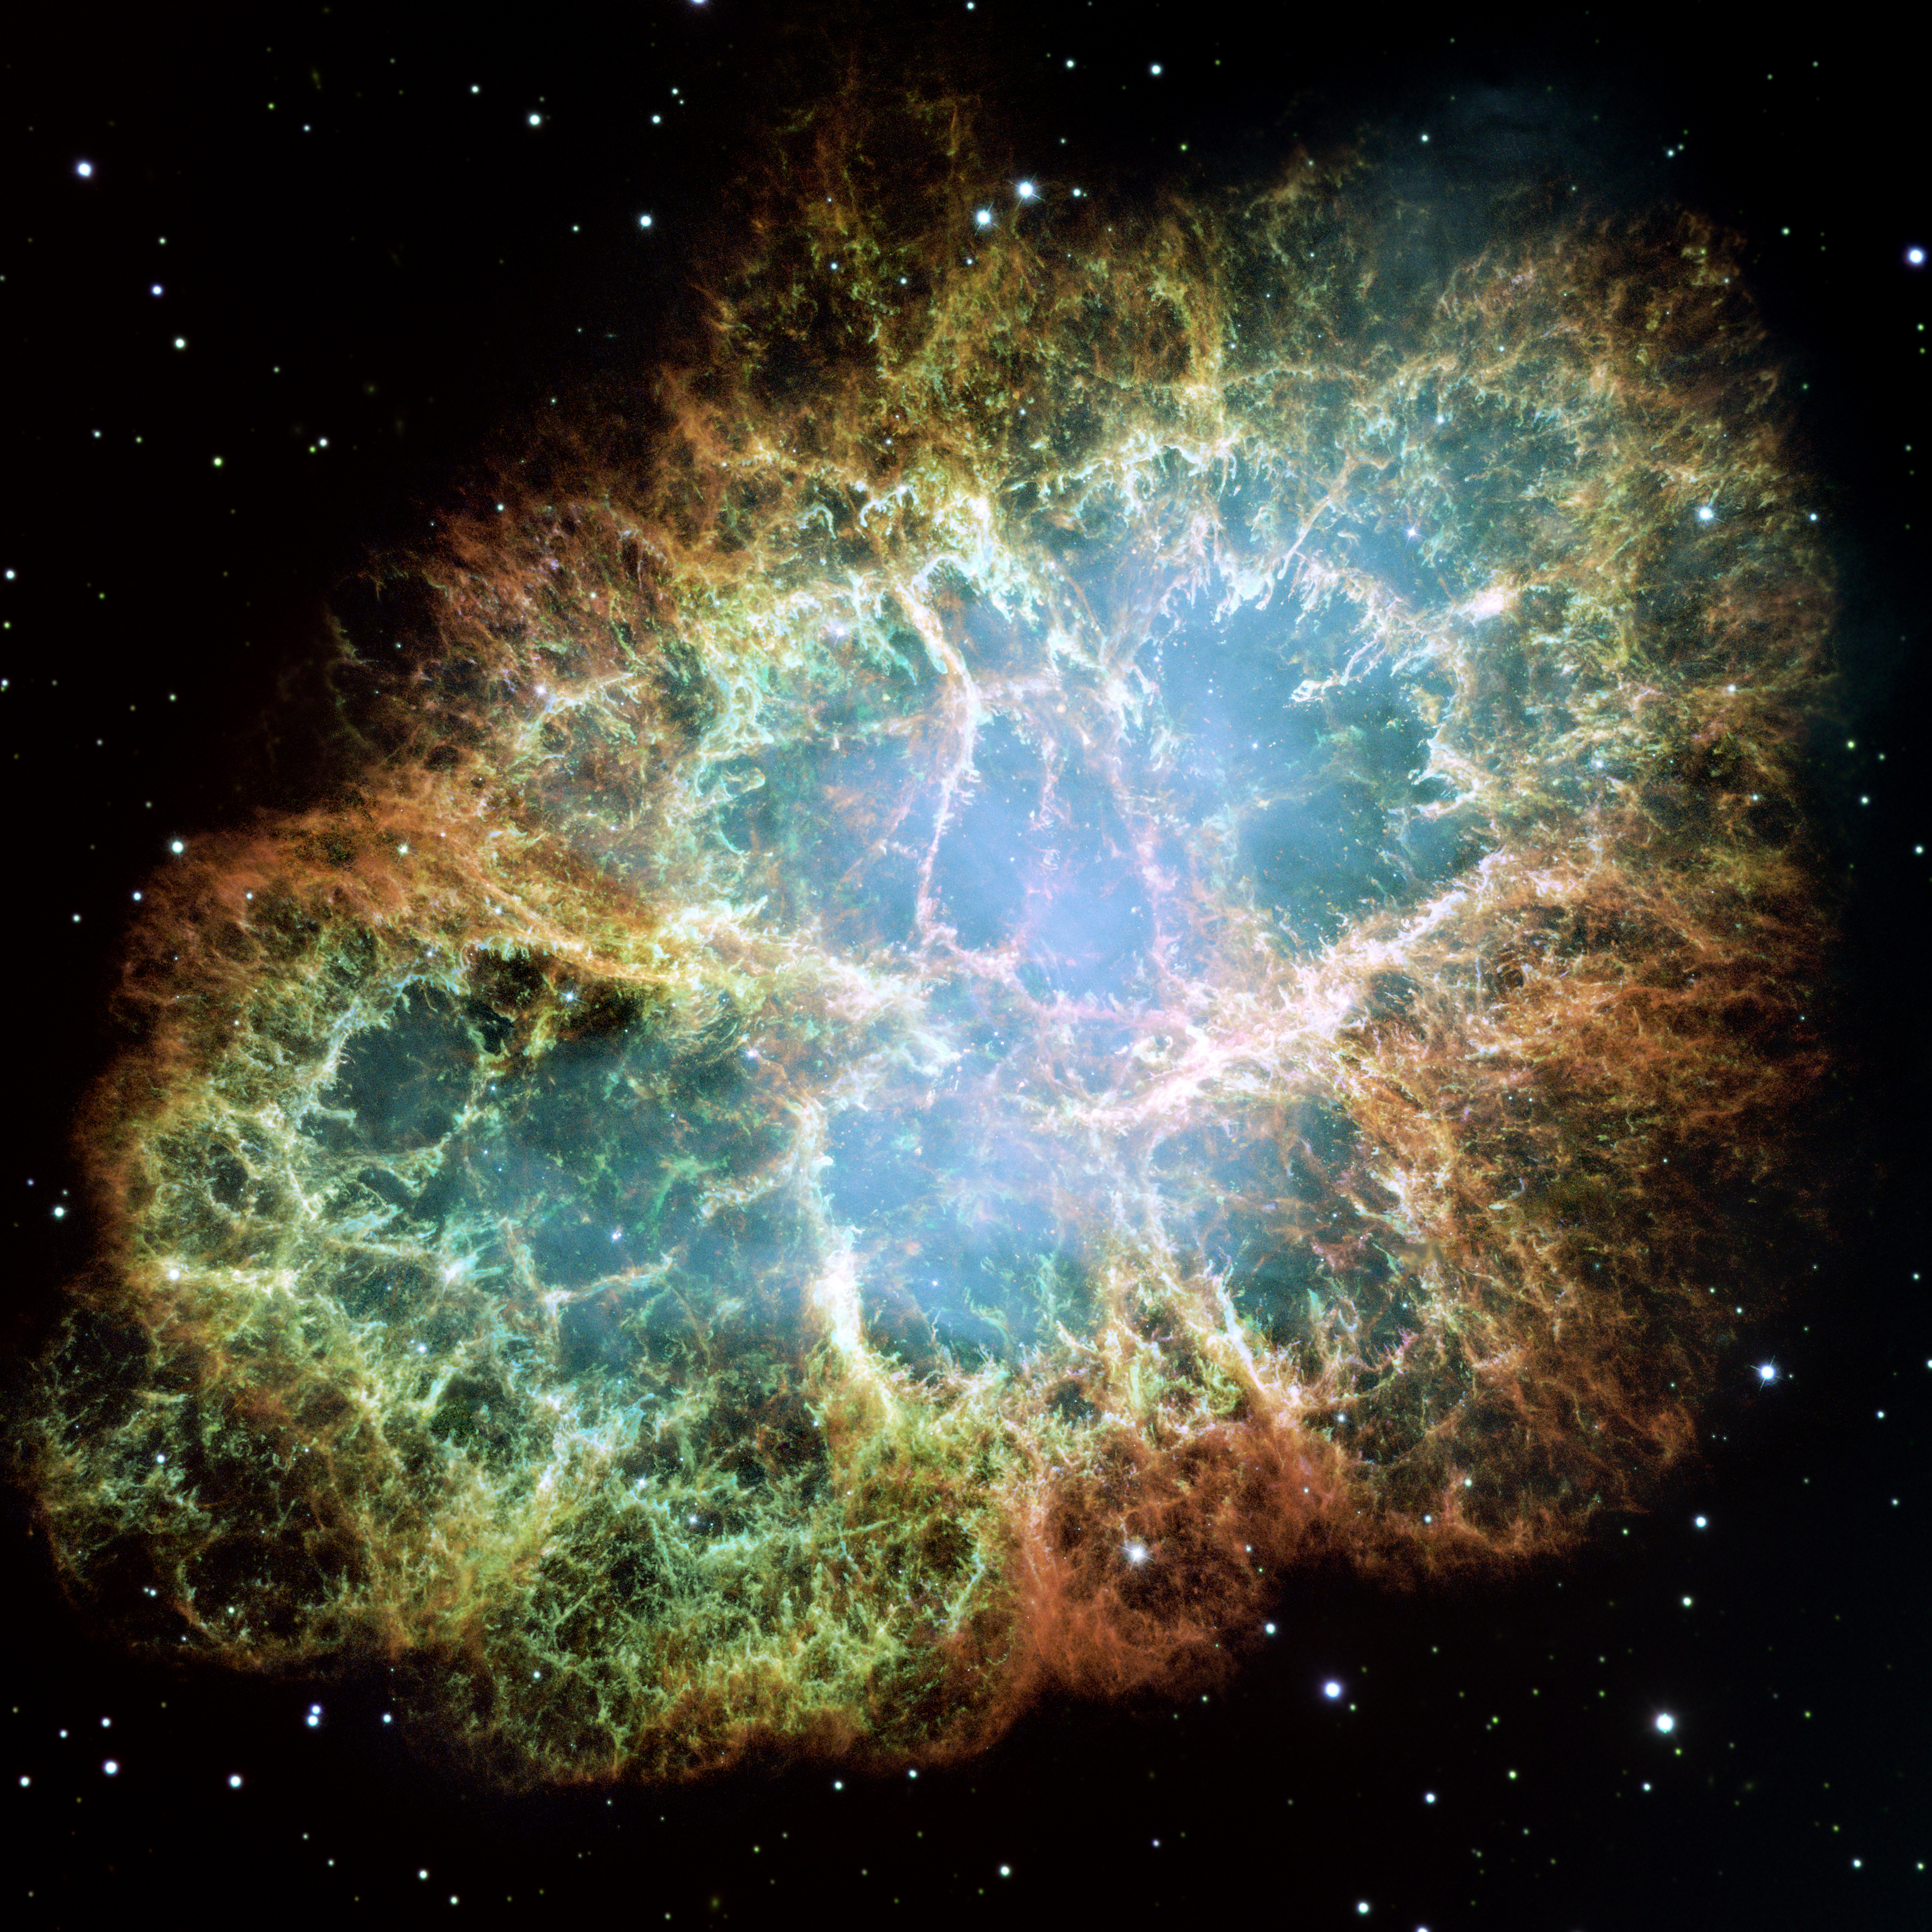
\includegraphics[width=0.56\textwidth]{img/crabnebula} 
\caption{Immagine della Nebulosa del Granchio.} \label{fig:Crab}
\end{center}
\end{figure}

In questo capitolo analizzeremo i principali processi di interazione radiazione-materia (tipicamente tra un fotone e un elettrone), studiando i processi di assorbimento, emissione, e scattering. Processi di assorbimento ed emissione sono processi in cui viene scambiata energia tra materia e radiazione. Tra questi ultimi si distinguono i processi \textit{free-free} (la carica è libera sia prima che dopo l'interazione con la radiazione), \textit{bound-free} (la carica si trova legata prima dell'interazione ed è libera dopo l'interazione, o viceversa), e \textit{bound-bound} (la carica è legata sia prima che dopo l'interazione con la radiazione. Ad esempio le righe spettrali sono dovute a questi processi). I processi di scattering consistono invece in una deviazione della traiettoria del fotone: tra questi si distinguono lo scattering \textit{Rayleigh}, \textit{Thomson} in cui non si ha scambio di energia tra fotone ed elettrone interagente, e scattering \textit{Compton} in cui elettrone e fotone scambiano energia durante la loro interazione. Prima di affrontare nel dettaglio questi processi, presentiamo alcuni rudimenti di elettromagnetismo per chiarire il formalismo adottato e presentare le basi della trattazione successiva. Il testo di riferimento per questo capitolo è \citep{book:Rybicki}.



\section{Radiazione}
La luce, come onda elettromagnetica, viene caratterizzata da frequenza $\nu$, frequenza angolare $\omega$, periodo $T$, lunghezza d'onda $\lambda$, numero d'onda $k$, velocità $c$. Di seguito sono riportate le principali relazioni tra queste grandezze.
\begin{align*}
\omega &= 2\pi \nu \\
T &= \inv{\nu} \\
k &= \dfrac{2\pi}{\lambda}\\
c &= \lambda\nu \approx 3\cdot 10^{10} \, \mathrm{cm}/\mathrm{s}
\end{align*}
La tabella \ref{tab:spettro} riporta la suddivisione dello spettro elettromagnetico in bande di frequenza e lunghezza d'onda, riportando inoltre i telescopi che lavorano nelle varie bande e gli oggetti tipici che emettono principalmente nella banda di interesse.
\begin{table}
\begin{center}
\begin{tabular}{ccccc}
\toprule
Banda &$\lambda$ & $\nu$ & Energia & Osservatori \\
\midrule \\[0.4ex]
Radio & $>10 \um{c}$ & $\leq 250 \uHz{M}$ &$<1\,\mu\mathrm{eV}$ & VLA, SKA \\[2pt]
Microonde & $10 \um{c} - 1 \um{m}$ & $ 250 \uHz{M} - 300 \uHz{G}$ &$1\,\mu\mathrm{eV} - 1.2 \ueV{m}$ & ALMA\\[2pt]
Infrarosso & $1 \um{m} - 700 \um{n}$ & $ 300 \uHz{G} - 428 \uHz{T}$ &$ 1.2 \ueV{m} - 1.8 \ueV{}$ & Spitzer, Hershel\\[2pt]
Visibile & $700 \um{n} - 400 \um{n}$ & $ 428 \uHz{T} - 749 \uHz{T}$ &$1.8 \ueV{} - 3.1 \ueV{}$ & Hubble, VLT\\[2pt]
Ultravioletto & $400 \um{n} - 10 \um{n}$ & $ 749 \uHz{T} - 30 \uHz{P}$ &$3.1 \ueV{} - 124 \ueV{}$ & Hubble\\[2pt]
X& $10 \um{n} - 1 \um{p}$ & $ 30 \uHz{P} - 300 \uHz{E}$ &$124 \ueV{} - 1.24 \ueV{M}$ & Swift, Chandra, ATHENA\\[2pt]
Gamma& $< 1 \um{p}$ & $ > 300 \uHz{E}$ &$>1.24 \ueV{M}$ & IACT\\[2pt]
\bottomrule
\end{tabular} 
\end{center}
\caption{La tabella riporta la principale suddivisione dello spettro elettromagnetico, indicando le energie associate e i più importanti strumenti che operano in tali bande.} \label{tab:spettro}
\end{table}



\subsection{Equazioni di Maxwell}\label{sec:EqMaxwell}
In questo corso adotteremo il sistema $cgs$: le equazioni di Maxwell in questo sistema sono
\begin{EQ}
\begin{equation}
\begin{cases}
\Div{D} = 4\pi\rho \\
\Div{B} = 0 \\
\Rot{E} = -\inv{c}\derP{\V{B}}{t} \\[10pt]
\Rot{H} = \inv{c}\derP{\V{D}}{t} + \dfrac{4\pi}{c} \V{J}
\end{cases} \label{eq:Maxwell1}
\end{equation}
\end{EQ}
dove $\V{D}$ è il campo di induzione elettrica, $\rho$ è la densità di carica elettrica, $\V{B}$ è il campo di induzione magnetica, $\V{E}$ è il campo elettrico mentre $\V{H}$ è il campo magnetico. Le relazioni tra i campi di induzione e i campi sono
\begin{equation}
\begin{cases}
\V{D}= \varepsilon \V{E} \\
\V{B}=\mu \V{H}
\end{cases}
\end{equation}
dove $\varepsilon$ è la costante dielettrica, mentre $\mu$ è la permeabilità magnetica. Nel sistema cgs sono costanti adimensionali che valgono $1$ nel vuoto. Notiamo inoltre che in questo sistema campo elettrico e magnetico hanno le stesse dimensioni. In questo caso le equazioni si riducono a
\begin{EQ}
\begin{equation}
\begin{cases}
\Div{E} = 0 \\
\Div{B} = 0 \\
\Rot{E} = -\inv{c}\derP{\V{B}}{t} \\[10pt]
\Rot{B} = \inv{c}\derP{\V{E}}{t} 
\end{cases} \label{eq:Maxwell2}
\end{equation}
\end{EQ}
 Combinando le equazioni di Maxwell si ottiene l'equazione di continuità della carica elettrica
\begin{EQ}
\begin{equation}
\derP{\rho}{t} + \Div{J} =0
\end{equation}
\end{EQ}
Concettualmente si può dire che le equazioni di Maxwell mostrano come le cariche generano i campi; il modo in cui i campi agiscono su una carica è invece espresso dalla forza di Lorentz
\begin{EQ}
\begin{equation}
\V{F} = q\left(\V{E} + \dfrac{\V{v}}{c}\times\V{B}\right) \label{eq:Lorentz}
\end{equation}
\end{EQ}
dove $q$ indica la carica singola.
Possiamo esprimere la forza di Lorentz per unità di volume
\begin{equation}
\V{f} = \rho\V{E} + \dfrac{\V{J}}{c}\times\V{B}
\end{equation}
Possiamo ora calcolare la potenza erogata dal campo elettromagnetico per accelerare una carica $q$. 
\begin{equation}
\der{W}{t} = \scal{f}{v} =\footnote{Questo mostra che il lavoro è fatto dal solo campo elettrico, non da quello magnetico.} \rho \scal{v}{E} = \scal{J}{E} =\footnote{In questo passaggio sostituiamo la quarta equazione di Maxwell.} \dfrac{c}{4\pi}(\Rot{H})\cdot\V{E} - \inv{4\pi}\derP{\V{D}}{t}\cdot\V{E} 
\end{equation}
Sfruttando la proprietà $\Div{}(\vett{A}{C}) = \scal{C}{}(\Rot{A})-\scal{A}{}(\Rot{C})$ otteniamo
\begin{equation}
\der{W}{t} = \dfrac{c}{4\pi}\Div{}(\vett{H}{E}) + \dfrac{c}{4\pi} \scal{H}{}(\Rot{E}) -\inv{4\pi} \derP{\V{D}}{t}\scal{}{E} = \dfrac{c}{4\pi}\Div{}(\vett{H}{E}) - \inv{8\pi} \derP{}{t}(\scal{B}{H}+\scal{D}{E})
\end{equation}
dove nell'ultimo passaggio abbiamo utlizato la terza equazione di Maxwell e raccolto i termini con derivata temporale. A questo punto definendo 
\begin{EQ}
\begin{align}
&\V{S} \equiv \dfrac{c}{4\pi} \vett{E}{H}
&U \equiv \inv{8\pi}(\scal{E}{D} + \scal{B}{H})
\end{align}
\end{EQ}
otteniamo un importante risultato dell'elettromagnetismo
\begin{EQ}
\begin{equation}
\derP{\V{U}}{t}+\Div{S} = - \der{W}{t}
\end{equation}
\end{EQ}
Questa equazione è l'equazione di continuità della grandezza $U$, ovvero la densità di energia del campo elettromagnetico. Il flusso di questa quantità e il \textit{vettore di Poynting} $\V{S}$. Vediamo che nell'accelerare una carica, il campo elettromagnetico perde energia.

Un altro importante risultato dell'elettromagnetismo è ottenibile combinando le equazioni \ref{eq:Maxwell2}, sfruttando le identità degli operatori vettoriali:
\begin{equation}
\Rot{}(\Rot{E})=\Grad(\Div{E}) - \Grad^2\V{E} = -\inv{c}\derP{}{t}(\Rot{B}) = -\inv{c^2}\derPn{\V{E}}{t}{2}
\end{equation}
Procedendo analogamente per $\V{B}$ otteniamo le equazioni delle onde per il campo elettrico e magnetico
\begin{EQ}
\begin{align}
&\Grad^2 \V{E} -\inv{c^2}\derPn{\V{E}}{t}{2} = 0
&\Grad^2 \V{B} -\inv{c^2}\derPn{\V{B}}{t}{2} = 0
\end{align}
\end{EQ}
le cui soluzioni sono onde piane del tipo
\begin{EQ}
\begin{align}
&\V{E}=\V{E}_0 e^{i(\scal{k}{r}-\omega t)}
&\V{B}=\V{B}_0 e^{i(\scal{k}{r}-\omega t)}
\end{align}
\end{EQ}
Questo risultato mostra che nel vuoto le variazioni del campo elettrico e magnetico si autosostengono, propagando come onde dette onde elettromagnetiche. Sostituendo le onde piane nelle prime due equazioni di Maxwell si trova che $\scal{k}{E}_0=0$ e $\scal{k}{B}_0=0$ cioè che le onde elettromagnetiche sono trasversali alla direzione di propagazione. Infine sostituendo le onde piane nelle ultime due equazioni si trova 
\begin{align}
&\vett{k}{E}_0 = \dfrac{\omega}{c} \V{B}_0
&\vett{k}{B}_0 = \dfrac{\omega}{c} \V{E}_0
\end{align}
che implica che il campo elettrico e il campo magnetico dell'onda sono ortogonali tra loro; inoltre dalle due relazioni precedenti si ottiene la relazione di dispersione delle onde elettromagnetiche, $\omega^2=k^2c^2$, da cui risulta che nel vuoto i moduli del campo elettrico e magnetico sono uguali, ovvero $\V{E}_0=\V{B}_0$. Da ciò segue anche che 
\begin{EQ}
\begin{align}
&U\inv{4\pi}E_0^2 = \inv{4\pi}B_0^2
&\V{S} = \dfrac{c}{4\pi} E_0^2 \vers{k} = Uc\vers{k}
\end{align}
\end{EQ}
L'ultima uguaglianza mostra che il flusso del campo elettromagnetico (il vettore di Poynting) è dato dalla densità di energia per la velocità della luce (velocità di propagazione dell'onda) nella direzione di propagazione $\vers{k}$.

Se la variazione di direzione di $\zeta$ (vettore funzione d'onda) nel piano ortogonale alla propagazione in funzione della coordinata spaziale di propagazione e del tempo può essere espressa da una legge (funzione), si dice che l'onda è polarizzata. 
In generale un'onda elettromagnetica è data dalla sovrapposizione di più onde, non necessariamente in fase tra loro
\begin{equation}
\V{E}=\V{E}_1 e^{i\omega t} + \V{E}_2 e^{i\omega t} e^{i\phi}
\end{equation}
dove i campi $\V{E}_1$ e $\V{E}_2$ contengono l'ampiezza e il termine di propagazione spaziale. Se $\V{E}_1=\V{E}_2$ e $\phi=0$ l'onda è polarizzata linearmente, ovvero i campi oscillano su una linea appartenente al piano ortogonale alla direzione di propagazione. Se $\V{E}_1=\V{E}_2$ e $\phi = \pm \pi/2$ la polarizzazione è circolare: se $\phi=+\pi/2$ si ha polarizzazione sinistra (il vettore ruota in senso antiorario), se $\phi=-\pi/2$ si ha polarizzazione destra (il vettore ruota in senso orario). Infine se $\V{E}_1\neq\V{E}_2$ ma $\phi = \pm \pi/2$ l'onda ha polarizzazione ellittica. 
Il caso ancora più generico è quello in cui il campo è dato dalla sovrapposizione di più onde a frequenze $\omega$ differenti.

\subsection{Spettro}
Con \textit{spettro di una radiazione} si indica l'insieme delle frequenze di cui è composta la radiazione elettromagnetica osservata.
Lo spettro della radiazione dipende dalla variazione temporale del campo elettrico (ignoriamo per semplicità il campo magnetico poichè le sue variazioni dipendono da quelle del campo elettrico). Una conseguenza di ciò è che non è possibiile dare un significato preciso allo spettro di una radiazione in un dato istante di tempo sapendo solo il campo elettrico in un punto. Occorre invece parlare di spettro di un treno d'onda o di radiazione in un punto in un lungo intervallo di tempo $\Delta t$. Se si dispone di un tempo di osservazione del campo della radiazione $\Delta t$, è possibile definire lo spettro con una risoluzione di frequenza $\Delta \omega$, con $\Delta \omega \, \Delta t >1$. Questa relazione di indeterminazione non è necessariamente quantistica, ma è comunque una proprietà alla base di ogni teoria ondulatoria della luce. Questa relazione implica che quanto più grande è il tempo di osservazione della radiazione, tanto più sarà dettagliata la nostra conoscenza dello spettro, ovvero della frequenza $\Delta\omega$.


%Assumioamo per semplicità matematica, che la radiazione sia nella forma di un impulso finito (in pratica richiediamo che il campo elettrico $\V{E}(t)$ si annulli rapidamente per $t\longrightarrow\pm\infty$). Inoltre 

Prima di discutere lo spettro della radiazione, ricordiamo che data una funzione del tempo $a(t)$, è possibile esprimerla in termini della trasformata di Fourier $\tilde{a}(\omega)$
\begin{EQ}
\begin{align}
&a(t) = \int_{-\infty}^{+\infty}\tilde{a}(\omega)\,e^{-i\omega t} \dd\omega
&\tilde{a}(\omega) = \inv{2\pi}\int_{-\infty}^{+\infty}a(t)\,e^{i\omega t} \dd t
\end{align}
\end{EQ}
Ricordiamo il teorema di Parseval
\begin{EQ}
\begin{equation}
\int_{-\infty}^{+\infty} a^2(t) \dd t = 2 \pi \int_{-\infty}^{+\infty} |\tilde{a}(\omega)|^2 \dd \omega
\end{equation}
\end{EQ}
Inoltre un'utile proprietà è che se $a(t)$ è reale, allora si ha
\begin{align}
\tilde{a}(-\omega) &= \inv{2\pi} \int_{-\infty}^{+\infty} a(t)\, e^{-i\omega t} \dd t = \\
&=\inv{2\pi} \int_{-\infty}^{+\infty} a^*(t)\, e^{-i\omega t} \dd t = \\
&= \tilde{a}^{*}(\omega) \label{eq:Spettro1}
\end{align}
dove $*$ indica il complesso coniugato. 

La trasformata di Fourier del campo elettrico $\hat{\V{E}}(\omega)$ contiene tutte le informazioni sulla dipendenza dalla frequenza del campo elettrico $\V{E}(t)$; infatti non è altro che il campo elettrico nel dominio delle frequenze. Per ottenere la dipendenza dalla frequenza dell'energia della radiazione, possiamo scrivere il flusso della radiazione (cioè l'energia che transita attraverso la superficie unitaria nell'unità di tempo) tramite il vettore di Poynting
\begin{equation}
\dfrac{\dd W}{\dd t \, \dd A} =  |\V{S}| = \dfrac{c}{4 \pi} |\V{E}(t)|^2
\end{equation}
A questo punto integriamo su tutti i tempi, e sfruttando il teorema di Parseval e la proprietà \ref{eq:Spettro1}, otteniamo
\begin{equation}
\der{W}{A} = \dfrac{c}{4\pi} \int_{-\infty}^{+\infty} |\V{E}(t)|^2 \dd t = \dfrac{c}{2} \int_{-\infty}^{+\infty} |\hat{\V{E}}(\omega)|^2 \dd \omega = c \int_{0}^{+\infty} |\hat{\V{E}}(\omega)|^2 \dd \omega
\end{equation}
Possiamo così identificare l'energia per unità di area e di frequenza con
\begin{EQ}
\begin{equation}
\dfrac{\dd W}{\dd A \, \dd \omega} = c |\hat{\V{E}}(\omega)|^2
\end{equation}
\end{EQ}
Sottolineaiamo il fatto che questa è l'energia totale per unità di area e di frequenza di un intero impulso; non abbiamo scritto "per unità di tempo". Infatti per scrivere sia $\dd t$ che $\dd\omega$ violeremmo il principio di indeterminazione tra $\omega$ e $t$. Tuttavia se l'impulso si ripete con un periodo $T$, allora è possibile scrivere formalmente 
\begin{equation}
\dfrac{\dd W}{\dd A \, \dd \omega \, \dd t} \equiv \inv{T} \dfrac{\dd W}{\dd A \, \dd \omega} = \dfrac{c}{T} |\V{E}(\omega)|^2
\end{equation}
Questa formula può essere usata per definire lo spettro di una porzione di lunghezza $T$ di un segnale molto più lungo. Se un segnale ha più o meno le stesse proprietà lungo tutta la sua durata (cioè è stazonario), allora ci aspettiamo che il risultato sia indipendente da $T$ per grandi $T$, e possiamo scrivere
\begin{equation}
\dfrac{\dd W}{\dd A \, \dd \omega \, \dd t}  = c \lim_{T\to\infty} \inv{T} |\hat{\V{E}}_T(\omega)|^2
\end{equation}
dove la scrittura $\hat{\V{E}}_T(\omega)$ serve a enfatizzare il fatto che è la trasformata di Fourier di una porzione di lunghezza $T$ della funzione $\V{E}$. In questo modo possiamo generalizzare la discussione fino ad includere onde infinitamente lunghe (come onde sinusoidali) usando formule basate su quelle ottenute per un impulso finito. Se le proprietà di $\V{E}(t)$ variano nel tempo, ci sia aspetta che lo spettro determinato dall'analisi di una porzione di lunghezza $T$ dipenda solo dalla porzione analizzata. In questo caso il concetto di spettro locale avrà senso se la variazione del campo $\V{E}(t)$ avviene su una scala temporale abbastanza lunga da poter definire un intervallo $T$ in cui si può ottenere una risoluzione di frequenza $\Delta \omega$ tale che $\Delta\omega \sim 1/T$. Se questa condizione non è soddisfatta la definizione di uno spettro locale non è utile, e occorre considerare lo spettro di tutto l'impulso come entità di base. Consideriamo ora alcuni impulsi tipici e i loro spettri corrispondenti (figura \ref{fig:Impulso1}, \ref{fig:Impulso2}, \ref{fig:Impulso3}). Studi come questo permettono di ottenere informazioni sulle relazioni utili nella stima degli spettri di un particolare processo. Notiamo che l'estensione dell'impulso $T$ determina la larghezza della più fine struttura risolvibile nello spettro: più grande è $T$, più stretto è il picco nel dominio delle frequenze. Inoltre notiamo che una dipendenza sinusoidale dal tempo causa un picco nel dominio delle frequenze centrato in $\omega_0$. Per $T\to\infty$ (dove, ricordiamo, $T$ è il tempo di osservazione dell'impulso, non il periodo della sinusoide) lo spettro tende ad una delta di Dirac centrata in $\omega_0$.
\begin{figure}
\includegraphics[width=\textwidth]{img/Impulso1}
\caption{Impulso gaussiano di larghezza $T$.}\label{fig:Impulso1}
\end{figure}
\begin{figure}
\includegraphics[width=\textwidth]{img/Impulso2}
\caption{Impulso sinusoidale $\sin \omega_0 t$.}\label{fig:Impulso2}
\end{figure}
\begin{figure}
\includegraphics[width=\textwidth]{img/Impulso3}
\caption{Impulso sinusoidale con smorzamento $\exp{-t/T}$.}\label{fig:Impulso3}
\end{figure}

\section{Radiazione da carica accelerata}
La derivazione canonica delle equazioni che descrivono la radiazione generata da una carica accelerata parte dalle equazioni di Maxwell e richiede di scrivere i potenziali ritardati del campo elettrico e magnetico, in un punto distante $\V{r}$ dalla carica. È tuttavia più istruttivo seguire l'approccio di Thomson \citep{book:Longair}, che mostra più chiaramente l'origine fisica della radiazione di una carica accelerata.

Consideriamo una carica $q$ stazionaria nell'origine $O$ di un sistema di riferimento inerziale $S$ al tempo $t=0$. Supponiamo che la carica subisca una piccola accelerazione alla velocità $\Delta v$ in un breve intervallo di tempo $\Delta t$. Thomson visualizzò il campo risultante in termini delle linee di campo, come mostrato in figura \ref{fig:Radiazione1}.
\begin{figure}
\begin{center}
\includegraphics[width=0.8\textwidth]{img/CaricaAccelerata}
\caption{Schema delle linee di campo associate ad una carica accelerata. La figura è discussa nel testo.} \label{fig:Radiazione1}
\end{center}
\end{figure}
Dopo un tempo $t$ possiamo distinguere tra la configurazioni dentro e fuori la sfera di raggio $r=ct$ centrata in $O$ poichè le perturbazioni del campo elettromagnetico propagano a velocità $c$ nel vuoto. Fuori dalla sfera, l'informazione dello spostamento della carica da $O$ non è ancora pervenuta, poichè appunto tale informazione viaggia alla velocità della luce. Tra queste due regioni abbiamo un sottile guscio di spessore $c\Delta t$ in cui si devono congiungere le corrispondenti linee di campo. Geometricamente è chiaro che ci deve essere una componente del campo elettrico in direzione tangenziale, ovvero in direzione $\hat{\V{\theta}}$. L'impulso del campo elettromagnetico è propagato dalla carica a velocità $c$, e corrisponde alla perdita di energia impiegata per accelerare la carica. 
Studiamo ora questo impulso del campo elettrico che sta propagando nello spazio. Assumiamo anzitutto che l'incremento di velocità $\Delta v$ subito dalla carica sia molto piccolo, ($\Delta v \ll c$, ovvero regime non relativistico), potendo così assumere che le linee di campo sono radiali nel sistema $S$ non solo a $t=0$ ma anche al tempo $t$. Consideriamo la linea di campo ad un angolo $\theta$; congiungiamo le linee di campo attraverso il guscio di spessore $c\Delta t$. Dalla geometria del sistema risulta che 
\begin{equation}
\dfrac{{E}_\theta}{{E}_r} = \dfrac{\Delta v \, t \sin \theta}{\Delta t \,c} = \dfrac{a\,r}{c^2} \sin\theta
\end{equation}
dove $a$ è il modulo dell'accelerazione subita dalla carica. Essendo poi noto il campo radiale $\V{E}_r = q/r^2 \,\V{r}$, otteniamo il \textit{campo di radiazione}
\begin{EQ}
\begin{equation}
E_\theta = \dfrac{q \,a}{rc^2} sin\theta
\end{equation}
\end{EQ}
Notiamo che la componente radiale del campo decresce come $r^{-2}$, in accordo con la legge di Coulomb, mentre la componente tangenziale decresce solo come $r^{-1}$; ciò è in accordo col fatto che l'intensità di un'onda (ovvero il suo vettore di Poynting) è proporzionale a $E^2$ e che l'intensità di un'onda sferica decresce come $r^{-2}$. Notiamo infine che il modulo del campo di radiazione è direttamente proporzionale all'acelerazione della carica, e dipende dall'angolo considerato (si ha un minimo nella direzione dell'accelerazione e un massimo nella direzione ortogonale all'accelerazione).
Consideriamo ora $\vers{n}$ direzione di propagazione, e indichiamo con il pedice rad i campi di radiazione: geometricamente si ha
\begin{align}
&\V{E}_\mathrm{rad} = \dfrac{q}{rc^2} \vers{n}\times(\vett{\hat{n}}{a})
&\V{B}_\mathrm{rad} = \vers{n}\times \V{E}_\mathrm{rad} = - \dfrac{(\vett{\hat{n}}{a})q}{rc^2}
\end{align}
In generale il campo radiativo al tempo $t$ è funzione dell'accelerazione calcolata al tempo $(t-r/c)$ poichè l'informazione contenuta nel guscio sferico propaga a velocità $c$. Possiamo ora calcolare il vettore di Poynting, ottenendo la \textit{formula di Larmor} per unità di superficie
\begin{EQ}
\begin{equation}
\dfrac{\dd W}{\dd t \, \dd A} = |\V{S}| = \dfrac{c}{4\pi} E_\mathrm{rad}^2 = \dfrac{q^2 |\vett{\hat{n}}{a}|^2}{4\pi c^3 r^2} = \dfrac{q^2 a^2 \sin^2 \theta}{4\pi c^3 r^2} \label{eq:Larmor1}
\end{equation}
\end{EQ}
Riascivendo l'equazione in termini di angolo solido\footnote{La definizione di angolo solido è $\dd \Omega = \dfrac{\dd A}{r^2}$} otteniamo la \textit{formula di Larmor}
\begin{EQ}
\begin{equation}
\dfrac{\dd W}{\dd t \, \dd \Omega} = r^2|\V{S}| =\dfrac{q^2 |\vett{\hat{n}}{a}|^2}{4\pi c^3} = \dfrac{q^2 a^2 \sin^2 \theta}{4\pi c^3} \label{eq:Larmor2}
\end{equation}
\end{EQ}
Un'altra forma della formula di Larmor è quella ottenuta integrando su tutti gli angoli solidi. Il risultato fornisce la potenza totale emessa
\begin{EQ}
\begin{equation}
\der{W}{t} = \dfrac{2}{3} \dfrac{q^2 a^2}{c^3} \label{eq:Larmor3}
\end{equation}
\end{EQ}
La formula di Larmor, sia in forma differenziale che integrale, mostra che la potenza emessa è porporzionale al quadrato della carica e dell'accelerazione. Inoltre essa ha l'andamento tipico del dipolo ovvero la proporzionalità a $\sin^2 \theta$; non si ha emissione di radiazione lungo la direzione dell'accelerazione, e il massimo dell'emissione è in direzione perpendicolare all'accelerazione. 

Quando abbiamo a che fare con $N$ particelle in diverse posizioni $\V{r}_i$, velocità $\V{v}_i$ e carica $q_i$, possiamo calcolare il campo a grandi distanze semplicemente sovrapponendo tra loro i singoli $\V{E}_\mathrm{rad}$ associati a ciascuna particella. Tuttavia si ha una complicazione dovuta al fatto che la formula di Larmor ottenuta si riferisce a condizioni a tempi ritardati, e ciascuna particella ha tempi ritardati diversi. Un altro modo di vedere questa complicazione è che nel sovrapporre i campi di radiazione delle singole particelle dobbiamo tener conto delle differenze di fase dei diversi campi introdotte dai ritardi (causati dal fatto che le particelle occupano posizioni diverse). Questa complicazione può però essere eliminata soto opportune ipotesi. Supponiamo che il sistema abbia dimensione tipica $L$, e che la scala temporale su cui avviene l'accelerazione delle cariche sia $\tau$. Se $\tau\gg L/c$, ovvero se il tempo scala è molto più grande del tempo che la luce impiega a coprire la distanza tipica del sistema di cariche, allora le differenze tra i tempi di ritardo della sorgente sono trascurabili. Possiamo anche caratterizzare il tempo $\tau$ come la scala temporale oltre la quale si hanno cambiamenti significativi nel campo radiativo, scala temporale che determina la tipica frequenza della radiazione emessa. Chiamando $\nu$ tale frequenza si ha che $\nu = \tau^{-1}$. L'approssimazione $\tau\gg L/c$ può quindi essere riscritta come $\lambda\gg L$ con $\lambda$ lunghezza d'onda della radiazione. Pertanto se il sistema è piccolo in confronto alla l'unghezza d'onda della radiazione emessa, è possibile ignorare le differenze i ritardi temporali e quindi le differenze di fase tra i campi di radiazione dovuti alle singole cariche e calcolare il campo di radiazione totale come
\begin{equation}
\V{E}_\mathrm{rad} = \sum_{i=1}^N \dfrac{\vers{n}\times(\vett{\hat{n}}{\ddot{d}_i})}{r_i\, c^2}
\end{equation}
dove $\ddot{d}$ è la derivata temporale seconda del momento di dipolo elettrico della associato alla carica i-esima. Se siamo in \textit{approssimazione di dipolo}, ovvero se valgono le condizioni $\tau\gg L/c$ e $R\gg L$, con $R$ distanza dall'oggetto emittente si ha 
\begin{EQ}
\begin{equation}
\V{E}_\mathrm{rad} = \dfrac{\vers{n}\times(\vett{\hat{n}}{\ddot{D}})}{R\, c^2}
\end{equation}
\end{EQ}
avendo definito
\begin{equation}
\V{D}= \sum_{i=1}^N d_i
\end{equation}
Infine si può dimostrare (vedi \cite{book:Rybicki}) che l'energia emessa per unità di frequenza è 
\begin{EQ}
\begin{equation}
\der{W}{\omega} = \dfrac{8\pi}{3} \dfrac{\omega^4}{c^3} |\tilde{D}(\omega)|^2 \label{eq:Larmor4}
\end{equation}
\end{EQ}
dove $\tilde{D}(\omega)$ indica la trasformata di Fourier del momento di dipolo totale.

\subsection{Radizione di ciclotrone}\label{subsec:Ciclotrone}
Il ciclotrone è il caso relativistico del sincrotrone, trattato nella sezione \ref{subsec:Sincrotrone}, e consiste in una carica (tipicamente un elettrone, motivo per cui interscambieremo il termine carica con elettrone) in moto in un campo magnetico costante $\V{B}$. La carica $q$ di massa $m$ subisce un'accelerazione dovuta alla forza di Lorentz \ref{eq:Lorentz}. Per semplicità supponiamo che la carica si muova in un piano ortogonale al campo magnetico, orientato lungo $\vers{z}$. Otteniamo il sistema
\begin{align}
&\begin{cases}
m\,a_x &=  \dfrac{q \, B\, v_y}{c} \\[10pt]
m\,a_y &=  \dfrac{q \, B\, v_x}{c}
\end{cases}
&\Longrightarrow \,\,\,\,\,\,\,\,\,\,\,\,\,\,\,\,\,\,\,\,\,\,\,\,\,\,
&\begin{cases}
\ddot{v}_x &= -\left(\dfrac{q\, B\,}{m\, c}\right)^2 v_x \\[10pt]
\ddot{v}_y &= -\left(\dfrac{q\, B\,}{m\, c}\right)^2 v_y
\end{cases}
\end{align}
e si definisce la frequenza di ciclotrone come 
\begin{EQ}
\begin{equation}
\omega_\mathrm{c} = \dfrac{q\, B\,}{m\, c}
\end{equation}
\end{EQ}
Possiamo calcolare la potenza emessa sfruttando la formula di Larmor \ref{eq:Larmor3} (ponendo $a= \omega_\mathrm{c} v$) e definendo $\beta \equiv v/c $ otteniamo
\begin{equation}
\der{W}{t} = \dfrac{2}{3} r_0^2 \, c\,\beta^2\, B^2
\end{equation}
avendo definito 
\begin{equation}
r_0 \equiv \dfrac{q^2}{m c^2}
\end{equation}
raggio classico dell'elettrone, ovvero la distanza a cui il potenziale elettrostatico è uguale all'energia a riposo dell'elettrone. Se definiamo la densità di energia del campo magnetico $U_B$
\begin{equation}
U_B \equiv \dfrac{B^2}{8\pi}
\end{equation}
e la \textit{sezione d'urto Thomson} $\sigma_\mathrm{T}$ come 
\begin{EQ}
\begin{equation}
\sigma_\mathrm{T} \equiv \dfrac{8\pi}{3} r_0^2
\end{equation}
\end{EQ}
allora otteniamo la seguente espressione per la potenza di ciclotrone
\begin{EQ}
\begin{equation}
\der{W}{t} = \dfrac{2}{3}\beta^2\, r_0^2 \, c\, B^2 = 2 \beta^2 \, \sigma_\mathrm{T} c \, U_B \label{eq:Ciclotrone2}
\end{equation}
\end{EQ}
Il prodotto $c \, U_B$ è è il flusso dovuto al campo magnetico visto dall'elettrone; l'area di interazione tra elettrone e campo magnetico è $2 \beta^2 \, \sigma_\mathrm{T}$.
A questo punto definiamo $\theta$ come l'angolo compreso tra $\V{B}$ (che assumiamo orientato lungo l'asse $\vers{z}$) e la direzione di emissione $\vers{n}$, e senza perdita di generalità lo fissiamo nel piano $xz$, cioè $\vers{n}=(\sin\theta, 0, \cos\theta)$. L'accelerazione subita dall'elettrone è $\V{a} = a\vers{r}$ con $\vers{r} = (\cos\omega_\mathrm{c}t, \sin\omega_\mathrm{c}t, 0)$. Possiamo facilmente dimostrare che vale $|\vett{\hat{n}}{\hat{r}}|^2 = \cos^2\theta + \sin^2\theta \, \sin^2\omega_\mathrm{c}t$. A questo punto, mediando su un'orbita otteniamo $|\vett{\hat{n}}{\hat{r}}|^2 = \cos^2\theta + \inv{2}\sin^2\theta = \inv{2}(1+\cos^2\theta)$. Sostituendo questo termine nella formula di Larmor \ref{eq:Larmor2}, otteniamo la potenza di ciclotrone per unità di angolo solido 
\begin{EQ}
\begin{equation}
\dfrac{\dd W}{\dd t \, \dd \Omega}= \dfrac{1}{8\pi}\beta^2\, r_0^2 \, c\, B^2(1+\cos^2\theta) \label{eq:Ciclotrone1}
\end{equation}
\end{EQ}
Studiamo ora la polarizzazione considerando il campo magnetico di radiazione. Si ha che
\begin{equation}
\V{B}_\mathrm{rad} \propto \vett{\hat{n}}{a} \propto \vett{\hat{n}}{\hat{r}} = \cos\theta (-\sin\omega_\mathrm{c}t \, \vers{x} + \cos\omega_\mathrm{c}t \, \vers{y}) + \sin\theta \, \sin\omega_\mathrm{c}t \vers{z}
\end{equation}
Vediamo che se $\theta=\pi/2$, il campo è polarizzato linearmente, in quanto si ha oscillazione solo lungo la direzione $\vers{z}$. Invece se $\theta=0$ il campo è polarizzato circolarmente.

Tipicamente in presenza di un campo magnetico sono disponibili più cariche elettriche libere e quindi si hanno tante righe associate a diverse frequenze angolari $\omega_\mathrm{c}t$ (non chiaro, controllare su Jackson). Per emettere radiazione di ciclotrone è necessaria la presenza di un campo magnetico. Oggetti astrofisici che ce l'hanno sono ad esempio stelle di neutroni e nane bianche. Un sistema astrofisico che funge da ciclotrone è la \textit{polar}, una nana bianca circondata da un gas ionizzato, come ad esempio AM Herculis. I campi tipici di questi sistemi sono in un range di $1 - 8\cdot 10^{7}\,G$, corrispondenti ad una frequenza di emissione nell'ottico e nel vicino infrarosso. Nel caso delle stelle di neutroni si hanno invece campi magnetici molto più intensi, in un range compreso tra i $10^8 - 10^{15} \, \mathrm{G}$. Questo campo è molto più intenso poichè le stelle di neutroni sono più compatte (le nane bianche hanno raggi dell'ordine dei $10^8 \, \mathrm{cm}$, mentre le stelle di neutroni $10^6 \, \mathrm{cm}$); dovendosi conservare il flusso del campo magnetico, al termine del collasso gli oggetti più compatti presentano campi magnetici più intensi. Altri oggetti con intensi campi magnetici sono le \textit{X-ray binaries} come Her-X, con campi magnetici fino all'ordine di $10^{13} \, \mathrm{G}$ e righe spettrali nell'X.

\section{Scattering}
Nei processi di scattering elastico si ha l'interazione tra un fotone ed una carica (tipicamente un elettrone) senza trasferimento di energia: il fotone entrante ha la stessa energia di quello uscente, quindi la sua frequenza non cambia. Tali processi vengono descritti con un fotone incidente sulla carica, la carica, e un fotone uscente con una traiettoria differente da quella iniziale. Infatti l'unico effetto dello scattering elastico è una deviazione del fotone dalla sua traiettoria iniziale.

\subsection{Scattering Thomson} \label{subsec:Thomson}
Il regime in cui avviene scattering Thomson è $h\nu \ll \mel c^2$, ovvero l'energia del fotone deve essere molto più piccola della massa a riposo dell'elettrone. Un esempio astrofisico in cui si osserva questo effetto è l'interazione dei fotoni del fondo cosmico con gli elettroni di mezzi interposti. Consideriamo un elettrone di carica $q$ e massa $m$ e un'onda che propaga in direzione $\vers{x}$ verso l'elettrone. Quando tale onda incide l'elettrone inizia ad oscillare. In base a quanto visto nella sezione \ref{sec:EqMaxwell} abbiamo che i moduli dei campi elettrico e magnetico della radiazione sono uguali; pertanto essendo in regime non relativistico per cui vale $v\ll c$ abbiamo che la forza di Lorentz si riduce a $\V{F}=q \V{E}$, forza che accelera la carica facendola oscillare. Possiamo usare le formule di Larmor per calcolare la potenza della radiazione emessa dall'elettrone oscillante: ipotizzando che il campo elettrico sia nella forma $\V{E} = \V{E}_0 \cos \omega t$, la forza di Lorentz ci permette di ricavare l'accelerazione subita dall'elettrone $m\ddot{r} = q \V{E}_0 \cos\omega t$. Sostituendo l'accelerazione così ottenuta nella formula di Larmor \ref{eq:Larmor2}, mediando su un periodo di oscillazione dell'elettrone (che riduce il fattore $\cos^2\omega t$ in $1/2$), e integrando su tutto l'angolo solido si ottiene
\begin{equation}
< \der{W}{t} >= \dfrac{q^4}{3c^3m^2}E_0^2 \label{eq:Thomson1}
\end{equation}
dove le parentesi indicano la media su un periodo di oscillazione. Il flusso incidente sull'elettrone è invece dato dal modulo del vettore di Poynting associato all'onda incidente sull'elettrone, dato da
\begin{equation}
|\V{S}| = \dfrac{c E^2}{4\pi} = \dfrac{cE_0^2}{4\pi} \cos^2\omega t
\end{equation}
che mediato su un periodo di oscillazione vale 
\begin{equation}
<|\V{S}|> = \dfrac{c E_0^2}{8\pi} \label{eq:Thomson2}
\end{equation}
Definiamo la \textit{sezione d'urto Thomson} come la sezione d'urto che moltiplicata per il flusso di radiazione incidente dà la potenza riemessa dall'elettrone: definendola in questo modo e usando le equazioni \ref{eq:Thomson1} e \ref{eq:Thomson2} otteniamo 
\begin{EQ}
\begin{equation}
\sigma_\mathrm{T}\Big|_\mathrm{lin} = < \der{W}{t} > \, \inv{<|\V{S}|>} = \dfrac{8\pi}{3} r_0^2
\end{equation}
\end{EQ}
già incontrata nella sezione precedente. Con un procedimento analogo si ricava banalmente la sezione d'urto di Thomson differenziale
\begin{EQ}
\begin{equation}
\der{\sigma_\mathrm{T}}{\Omega} \bigg|_\mathrm{lin} = r_0^2 \sin^2\theta
\end{equation}
\end{EQ}
con $\theta$ angolo compreso tra la direzione della polarizzazione lineare (asse di oscillazione della carica) e la direzione $\vers{n}$ della radiazione uscente.
Vediamo quindi che è giustificata l'ipotesi di considerare solo elettroni come particelle che contribuiscono allo scattering. Difatti $\sigma_\mathrm{T} \propto m^{-1}$, pertanto particelle massicce come il protone hanno sezione d'urto molto più piccola, e quindi non contribuiscono significativamente allo scattering Thomson.

In questa discussione abbiamo considerato una radiazione incidente polarizzata linearmente; cosa succede se la polarizzazione è circolare? In questo caso si ha
\begin{equation}
|\V{S}|=<|\V{S}|> = \dfrac{c E_0^2}{4\pi}
\end{equation}
L'effetto di una radizione incidente polarizzata circolarmente è quello di imprimere all'elettrone un moto circolare, con accelerazione centripeta data da $m\omega^2 r = q E_0$, da cui si trova 
\begin{align}
&r = \dfrac{qE_0}{m\omega^2}
&v = \dfrac{q E_0}{m\omega}
\end{align}
Questo caso è analogo al ciclotrone in cui si ha una carica in moto circolare uniforme, con la differenza che ora l'asse di rotazione non è dato da un campo ma dalla direzione di propagazione dei fotoni, ovvero l'angolo $\theta$ è l'angolo di scattering $\phi$ compreso tra la direzione del fotone entrante e quello del fotone uscente. Si ottiene dalla formula di Larmor, analogamente al ciclotrone,
\begin{equation}
\dfrac{\dd W}{\dd t \, \dd \Omega}  = \dfrac{c E_0^2}{8\pi}r_0^2 (1+\cos^2\phi) \label{eq:Thomson3}
\end{equation}
Dividendo per il vettore di Poynting otteniamo la sezione d'urto differenziale, e integrando poi su tutto l'angolo solido otteniamo la sezione d'urto totale di Thomson per la radiazione polarizzata circolarmente 
\begin{EQ}
\begin{align}
&\der{\sigma_\mathrm{T}}{\Omega}\bigg|_\mathrm{circ} = \dfrac{r_0^2}{2} (1+\cos^2\phi)
&\sigma_\mathrm{T}\Big|_\mathrm{circ} = \dfrac{8\pi}{3}r_0^2
\end{align}
\end{EQ}
Integrando la \ref{eq:Thomson3} su tutto l'angolo solido si ottiene
\begin{equation}
\der{W}{t}= \dfrac{2}{3} r_0^2 c E_0^2 = \sigma_{T} c U_\mathrm{ph}
\end{equation}
analoga alla potenza della radiazione del ciclotrone \ref{eq:Ciclotrone2}. Quest'ultima è il caso statico (il campo $\V{B}$ è costante), mentra quella appena trovata è il caso variabile (il campo è dato dall'onda incidente. Vediamo quindi che la sezione d'urto totale è la stessa sia che la radiazione sia polarizzata linearmente che circolarmente. Le differenze tra i due casi stanno invece nella sezione d'urto differenziale e nell'angolo da cui dipende: Nel caso della polarizzazione lineare si ha $\theta$ angolo tra la polarizzazione e la direzione dell'onda uscente, mentre nel caso della polarizzazione si ha l'angolo $\phi$ tra la direzione dell'onda entrante e la direzione dell'onda uscente.

Studiamo infine il caso in cui la radiazione incidente non sia polarizzata; 
sappiamo che un fascio di luce non polarizzata, che propaga in direzione $\V{k}$, può essere espresso come sovrapposizione di due fasci polarizzati linearmente su due assi perpendicolari $\V{E}_1$ e $\V{E}_2$. Senza perdita di generalità consideriamo un sistema di assi orientati in modo da avere $\V{E}_1$ orientanto lungo l'asse $\vers{x}$ , $\V{E}_2$ orientanto lungo l'asse $\vers{y}$  e $\V{k}$ orientato lungo $\vers{z}$. Consideriamo poi, la direzione dell'onda uscente $\vers{n}$ giacente nel piano $\vers{x}, \vers{z}$ di modo che formi un angolo $\theta$ con $\V{E}_1$ e $\pi/2$ con $\V{E}_2$. L'angolo di scattering è invece $\phi\equiv\pi/2-\theta$. La sezione d'urto differenziale è data da una media delle sezioni d'urto associate allo scattering della radiazione polarizzata linearmente agli angoli $\theta$ e $\pi/2$
\begin{EQ}
\begin{align}
\der{\sigma_\mathrm{T}}{\Omega} \bigg|_{unpol} &= \inv{2}\left[ \der{\sigma_\mathrm{T}}{\Omega} \bigg|_\mathrm{lin}(\theta) + \der{\sigma_\mathrm{T}}{\Omega} \bigg|_\mathrm{lin}\left(\dfrac{\pi}{2}\right) \right] = \\
&=\dfrac{r_0^2}{2} (1+\sin^2\theta) = \\
&=\dfrac{r_0^2}{2} (1+\cos^2\phi) \label{eq:Thomson4}
\end{align}
\end{EQ}
Notiamo che la sezione d'urto differenziale dello scattering Thomson è simmetrica per riflessioni rispetto al piano di incidenza della radiazione, ovvero è simmetrica per riflessioni $\theta\to -\theta$. Inoltre la sezione d'urto totale di Thomson è la stessa sia che la radiazione sia o meno polarizzata. Definendo il tasso di polarizzazione $\Pi$ come il rapporto tra l'intensità della radiazione polarizzata e l'intensità della totale, si può dimostrare \citep{book:Rybicki} che per l'onda uscente vale
\begin{equation}
\Pi = \dfrac{1-\cos^2\phi}{1+\cos^2\phi}
\end{equation}
cioè lo stattering elettronico è in grado di polarizzare la radiazione. La direzione in cui si ha il massimo della polarizzazione corrisponde a $\phi = \pi/2$, mentre in corrispondenza di $\phi=0$ non si ha polarizzazione.

Nel processo di scattering, i fotoni incidenti trasferiscono una quantità di moto agli elettroni, che può essere interpretata come una \textit{pressione di radiazione} data dal vettore di Poynting diviso la velocità della luce. La Forza esercitata dai fotoni sugli elettroni sarà
\begin{equation}
\V{F} = \dfrac{\V{S}}{c}\sigma_\mathrm{T}
\end{equation}
Questa forza di radiazione gioca un ruolo molto importante in fenomeni astrofisici come il vento stellare. Supponiamo di avere una stella circondata da un gas ionizzato. Il vettore di Poynting associato alla stella sarà la sua luminosità (ovvera la sua potenza totale emessa) diviso la superficie sferica considerata, quindi la forza di radiazione esercitata della stella sugli elettroni del gas ionizzato sarà
\begin{equation}
\V{F_\mathrm{rad}} = \dfrac{L}{4\pi\,r^2 \, c}\,\sigma_\mathrm{T} \, \vers{r}
\end{equation}
mentre la forza di gravità subita sarà
\begin{equation}
\V{F}_\mathrm{grav} = -\dfrac{GM\mpr}{r^2}\,\vers{r}
\end{equation}
Da un semplice bilancio tra queste due forze si deduce che esiste una luminosità massima, detta \textit{luminosità di Eddington} oltre la quale il gas ionizzato è espulso.
\begin{equation}
L_\mathrm{Edd}= \dfrac{4\pi G \mpr M c}{\sigma_\mathrm{T}} = 1.26\times10^{38} \tonde{\dfrac{M}{M_\odot}} \mathrm{erg/s}
\end{equation}
Sottolineiamo il fatto che la forza di radiazione è esercitata prevalentemente sugli elettroni, poichè essi hanno sezione d'urto Thomson molto più grande di quella dei protoni, mentre la forza di gravità è esercitata prevalentemente sui protoni del plasma, poichè essi hanno massa molto più grande di quella degli elettroni. Il "legame" tra queste due forze è dovuto all'interazione Coulombiana tra elettroni e protoni del plasma, che resta globalmente neutro. Questo implica che se la luminosità stellare supera quella di Eddington il vento stellare disperde il plasma esterno, e può anche disperdere gli strati esterni della stella stessa.

\subsection{Scattering di Rayleigh}
In questo tipo di scattering si considerano elettroni legati al nucleo. Per la descrizione useremo un modello molto semplificato che però consente di dare una buona descrizione del fenomeno: si assume che l'elettrone sia legato da una forza elastica e che la sua oscillazione sia forzata da un'onda incidente. la forza subita dall'elettrone è quindi
\begin{equation}
m\,\ddot{x} = q\,E_0\,\cos\omega t - m\, \omega_0^2 x
\end{equation}
Esprimendo il coseno in forma di esponenziale complesso possiamo riscrivere l'equazione a patto di andare poi a sceglierne solo le soluzioni reali. La soluzione che otteniamo è
\begin{equation}
x(t) = \dfrac{q\,E_0}{m} \inv{\omega_0^2-\omega^2} e^{i\omega t}
\end{equation}
da cui possiamo facilmente ricavare $\ddot{x}$; utilizzando la formula di Larmor \ref{eq:Larmor3} otteniamo la potenza totale emessa\footnote{In questo calcolo al posto di $a^2$ sostituiamo la media temporale (ovvero l'integrale tra $-T/2$ e $T/2$ diviso $T$) del quadrato di $\ddot{x}$. Questo calcolo fa saltar fuori un fattore $1/2$.}
\begin{equation}
\der{W}{t} = \dfrac{q^4}{3c^3}\left(\dfrac{\omega^2}{\omega_0^2-\omega^2}\right)^2 \dfrac{E_0^2}{m^2}
\end{equation}
Analogamente a quanto fatto per lo scattering di Thomson definiamo la sezione d'urto di Rayleigh come l'area che moltiplicata per il flusso della radiazione incidente (il vettore di Poynting) dà la potenza riemessa dall'elettrone. Otteniamo così
\begin{equation}
\sigma_\mathrm{R} = \sigma_\mathrm{T} \dfrac{\omega^4}{(\omega^2-\omega_0^2)^2}
\end{equation}
Se nell'equazione del moto fosse presente anche un termine di smorzamento, $m\Gamma\dot{x}$, allora la sezione d'urto di Rayleigh diventa
\begin{EQ}
\begin{equation}
\sigma_\mathrm{R} = \sigma_\mathrm{T} \dfrac{\omega^4}{(\omega^2-\omega_0^2)^2 + \Gamma^2}
\end{equation}
\end{EQ}
Nel limite $\omega\ll\omega_0$ si ha $\sigma_\mathrm{R} = \sigma_\mathrm{T} (\omega/\omega_0)^4$, viceversa se $\omega\gg\omega_0$ le sezioni d'urto di Rayleigh e di Thomson coincidono. Nella figura \ref{fig:Rayleigh} sono relazionate le sezioni d'urto ti Thomson e Rayleigh in funzione della frequenza.
\begin{figure}
\begin{center}
\includegraphics[width=0.8\textwidth]{img/ScatteringRayleigh}
\caption{Scattering di Rayleigh. Andamento della sezione d'urto in unità della sezione d'urto di Thomson in funzione della frequenza in unità di $\omega_0$.} \label{fig:Rayleigh}
\end{center}
\end{figure}

Lo scattering di Rayleigh della componente blu della luce solare da parte delle molecole dell'aria è il motivo principale per cui il cielo appare di colore azzurro, a causa della forte dipendenza della sezione d'urto dalla frequenza ($\propto\omega^4$). La radiazione ad alte frequenze ha una sezione d'urto maggiore di quella a basse frequenze, e pertanto viene diffusa più facilmente. Affinchè si abbia scattering Rayleigh, l'energia della radiazione deve essere inferiore all'energia di legame dell'elettrone col nucleo. Considerato che i principali componenti dell'atmosfera sono $\mathrm{N}_2$ e $\mathrm{O}_2$ (rispettivamente il $78 \%$ e il $21\%$) con energia di dissociazione pari rispettivamente a $9.39\, \mathrm{eV}$ e $5.15 \, \mathrm{eV}$, corrispondenti a fotoni di frequenza $\nu=2376 \, \mathrm{THz}$ e $\nu=1245 \, \mathrm{THz}$, (la luce rossa ha frequenza $\nu=428 \, \mathrm{THz}$, mentre quella blu $\nu=749 \, \mathrm{THz}$), la luce visibile è in grado di fare scattering Rayleigh nell'atmosfera: le componenti blu vengono scatterate facendo apparire il cielo blu, mentre le rimanenti gialle no, e vengono viste solo in direzione del sole.

\section[Bremsstrahlung]{Bremsstrahlung\footnote{Si pronuncia Bremstràlun.}}
In generale la bremsstrahlung è un qualsiasi tipo di radiazione dovuta all'accelerazione subita da una particella carica, compresa la radiazione di sincrotrone, di ciclotrone, e l'emissione di elettroni e positroni nel decadimento beta. Tuttavia questo termine viene comunemente usato per indicare la radiazione emessa da un elettrone libero nella materia, in seguito all'accelerazione provocata dall'interazione coulombiana con uno ione. Spesso ci si riferisce alla bremsstrahlung emessa da una plasma con il termine di radiazione free-free, per il fatto che in questo caso le cariche interagenti (elettrone e ione che genera il campo coulombiano che interagisce con l'elettrone) sono libere, o per lo meno, non legate tra loro sia prima che dopo l'interazione.
In generale questo processo va studiato con un approccio quantistico poichè possono essere prodotti fotoni di energie comparabili a quelle della particella emittente. Tuttavia un approccio classico, sotto opportune ipotesi, permette di giungere a conclusioni corrette, a cui vengono successivamente agggiunti gli effetti quantistici. Seguiremo quindi questo approccio più semplice, e trascureremo gli effetti relativistici, in quanto studieremo elettroni a temperature non superiori a $T=10^9\uK{}$. 

Iniziamo notando che la bremsstrahlung di due particelle identiche è nulla perchè in questo caso il momento di dipolo $\sum q_i \V{r}_i$  è semplicemente proporzionale al centro di massa del sistema $\sum m_i \V{r}_i$, che è una costante del moto, e quindi l'elemento di matrice associato alla transizione associata all'emissione, è nullo (poichè lo stato iniziale e lo stato finale sono diversi tra loro, e quindi ortogonali). Pertanto le particele devono essere diverse, ipotizziamo un elettrone e un generico ione di carica $Zq$. La particella emittente è l'elettrone in quanto più leggero e quindi subente un'accelerazione maggiore dello ione di massa $M$. A causa di ciò possiamo considerare un sistema di riferimento in cui lo ione è fermo, e resta tale per tutta l'interazione, e l'elettrone si avvicina su una traiettoria rettilinea lungo $\vers{x}$ a velocità $v\ll c$, traiettoria che ha distanza minima dallo ione pari a $b$, noto come \textit{parametro d'impatto}. Questo processo non è altro che lo scattering di Rutherford. Assumiamo che l'angolo di scattering $\phi \approx 0$, e calcoliamo la variazione di velocità in direzione $\vers{y}$ ortogonale alla direzione iniziale dell'elettrone. Ipotizziamo che il moto lungo $\vers{x}$ resti imperturbato, e quindi che $\V{v}_\mathrm{i} = (v,\,0)$, e $\V{v}_\mathrm{f} = (v,\,\Delta v)$. Indicando con $\V{r}$ il vettore che congiunge lo ione all'elettrone e con $\theta$ l'angolo tra $\V{r}$ e $\vers{x}$, abbiamo da semplici considerazioni geometriche che $\sin\theta = b/r$, e che $\tan\theta = b/x$, avendo fissato l'origine dell'asse $\vers{x}$ nel punto di minima distanza dallo ione. La forza che accelera l'elettrone in direzione $\vers{y}$ non è altro che la componente in tale direzione della forza coulombiana
\begin{equation}
F_y = -\dfrac{q^2Z}{r^2}\sin\theta = - \dfrac{q^2Z}{b^2}\sin^3\theta 
\end{equation}
Possiamo ora calcolare la variazione di velocità
\begin{align}
\Delta v &=  \int_{-\infty}^{+\infty} \dfrac{F_y}{m} \dd t = \int_{-\infty}^{+\infty} \dfrac{F_y}{m} \dfrac{\dd x}{v} = -\int_{0}^{\pi} \dfrac{F_y}{m} \dfrac{b}{\sin^2\theta}\, \dd \theta = \dfrac{2 q^2 Z}{m v b} \label{eq:Bremss3}
\end{align}
da cui vediamo subito che l'ipotesi che la variazione di velocità si piccola, $\Delta v \ll v$ equivale a 
\begin{equation}
\dfrac{q^2 Z}{b} \ll \inv{2}mv^2 \label{eq:Bremss6}
\end{equation}
cioè che l'energia cinetica dell'elettrone deve essere molto più grande dell'energia coulombiana massima, cioè quella raggiunta alla distanza minima elettrone-ione.
In media un elettrone in moto in un plasma subisce un gran numero di deflessioni, in direzioni tutte egualmente probabili, pertanto mediamente l'elettrone prosegue su traiettoria rettilinea, ovvero $\Delta v$ ha media nulla. Ciò non vale invece per $\Delta v^2$; data $n$ densità numerica degli ioni, il flusso di ioni visto dall'elettrone è $n\V{v}$. L'area di interazione con ciascuno ione è l'anello $2\pi\,b\,\dd b$. Pertanto la variazione temporale della quantità $\Delta v^2$ è data da $\Delta v^2$ per le interazioni per unità di tempo, integrata sul numero totale delle interazioni.
\begin{equation}
\der{}{t}(\Delta v)^2 = \int_{b_\mathrm{min}}^{b_\mathrm{max}} \left( \dfrac{2 q^2 Z}{m v b} \right)^2 nv\, 2\pi\,b\,\dd b = \dfrac{8\pi \,q^4 Z^2 n}{m^2 v} \ln \Lambda \label{eq:Bremss1}
\end{equation}
dove abbiamo definito 
\begin{equation}
\ln \Lambda \equiv \int_{b_\mathrm{min}}^{b_\mathrm{max}} \dfrac{\dd b}{b}
\end{equation}
noto come logaritmo coulombiano. Quando la \ref{eq:Bremss1} è dell'ordine di $v^2/\tau = v^3/ \mfp$, dove con $\tau$ si indica il tempo trascorso il quale la variazione di $v^2$ è dell'ordine della $v^2$ iniziale, mentre $\mfp$ indica il cammino libero medio, allora possiamo ricavare 
\begin{equation}
\mfp =\left(\inv{2}mv^2\right)^2 \inv{2\pi Z^2 q^4} \inv{n} \inv{\ln \Lambda} \approx \dfrac{(kT)^2}{2\pi Z^2 q^4} \inv{n} \inv{\ln \Lambda}
\end{equation}
dove nell'ultimo passaggio abbiamo approssimato l'energia cinetica all'energia termica.
Alcuni esempi sono il centro del sole in cui si ha $n\approx10^{26}\um{c}^{-3}$, $T\approx 10^7\uK{}$ che implica $\mfp \approx 10^{-8}\um{c}$, mentre per il vento solare si ha si ha $n\approx10^{-3}\um{c}^{-3}$, $T\approx 10^5\uK{}$ che implica $\mfp \approx 5\cdot 10^{13}\um{c}$, che è dell'ordine della distanza Terra-Sole $1 \uAU{} = 1.5\cdot 10^{13}\um{c}$.

A questo punto possiamo studiare lo spettro associato alla bremsstrahlung ricorrendo all'equazione \ref{eq:Larmor4}. Iniziamo studiando il quadrato della derivata seconda del momento di dipolo $\V{\ddot{d}}= -q\V{\dot{v}}$. Calcolando la trasformata di Fourier di questa relazione, otteniamo\footnote{Il primo membro deriva dal fatto che possiamo scrivere il momento di dipolo in termini della sua trasformata di Fourier
\begin{align*}
\V{\ddot{d}} = \dern{}{t}{2} \V{d}(t) = \dern{}{t}{2} \int_{-\infty}^{+\infty} \V{\tilde{d}}(\omega) e^{-i\omega t} \, \dd \omega = -\int_{-\infty}^{+\infty} \omega^2\V{\tilde{d}}(\omega) e^{-i\omega t} \, \dd \omega 
\end{align*} 
Notiamo che l'ultimo membro è l'antitrasformata della quantità $-\omega^2\V{\tilde{d}}(\omega)$. Pertanto risulta che la trasformata di Fourier di $\V{\ddot{d}}$ è $-\omega^2\V{\tilde{d}}(\omega)$, in quanto vale la proprietà $F\{ F^{-1}a(t)\} = a(t)$.}
\begin{equation}
-\omega^2 \tilde{\V{d}} = - \dfrac{q}{2\pi} \int_{-\infty}^{+\infty} \V{\dot{v}} e^{i\omega t} \, \dd t \label{eq:Bremss2}
\end{equation} 
Da questa relazione possiamo ottenere i valori di $\tilde{\V{d}}$ nei limiti di alte e basse frequenze. Anzitutto notiamo che l'interazione tra elettrone e ione ha una durata finita; assumendo che l'interazione avviene alla distanza $b$ tra le due particelle, il tempo di interazione, chiamato \textit{tempo di collisione} è dell'ordine di $\tau=b/v$. Per alte frequenze ($\omega\tau\gg 1$) l'esponenziale della \ref{eq:Bremss2} oscilla rapidamente, e l'integrale è piccolo; nel caso delle basse frequenze ($\omega\tau\ll 1$) l'esponenziale è essenzialmente unitario, e l'integrale vale quindi $\Delta v$. In altre parole si ha
\begin{align}
\omega^2 \V{\tilde{d}}(\omega) = 
\begin{cases}
\dfrac{q}{2\pi} \Delta\V{v} \,\,\,\,\,\,\,\,\,\,\,\,\,\,\,\,\,\,\,\, \omega\tau \ll 1 \\[10pt]
0 \,\,\,\,\,\,\,\,\,\,\,\,\,\,\,\,\,\,\,\,\,\,\,\,\,\,\,\,\,\,\,\,\,\, \omega\tau \gg 1 
\end{cases} \label{eq:Bremss4}
\end{align}
Possiamo ora sostituire la \ref{eq:Bremss3} nella \ref{eq:Bremss4} e quest'ultima nella formula di Larmor \ref{eq:Larmor4}, ottenendo
\begin{align}
\der{W}{\omega} = 
\begin{cases}
\dfrac{8\,Z^2 \,q^6}{3\pi \,c^3 \, m^2 \, v^2 \,b^2} \,\,\,\,\,\,\,\,\,\,\,\,\,\,\,\,\,\,\,\, \omega\tau \ll 1 \\[10pt]
0 \,\,\,\,\,\,\,\,\,\,\,\,\,\,\,\,\,\,\,\,\,\,\,\,\,\,\,\,\,\,\,\,\,\,\,\,\,\,\,\,\,\,\,\,\,\,\,\,\,\,\,\, \omega\tau \gg 1 
\end{cases} \label{eq:Bremss5}
\end{align}
Vediamo quindi che, dalla relazione tra tempo di collisione e parametro d'impatto, si ha emissione per $\omega b \ll v$, e quindi a parametri d'impatto piccoli corrispondono alte frequenze di emissione, e viceversa.

La discussione fatta finora tratta l'emissione da un singolo elettrone; determiniamo ora lo spettro totale per un mezzo con densità numerica di ioni $n_\mathrm{i}$ e densità numerica di elettroni $n_\mathrm{e}$. Il flusso di elettroni (numero di elettroni incidenti sull'unità di superficie nell'unità di tempo) è semplicemente $n_\mathrm{e}\,v$, e l'area di interazione tra elettroni e un singolo ione è $2\pi \, b\, \dd b$. La potenza emessa per unità di frequenza e di volume sarà quindi
\begin{equation}
\dfrac{\dd W}{\dd \omega\,\dd V \, \dd t} = n_\mathrm{e} n_\mathrm{i} \int_{b_\mathrm{min}}^{b_\mathrm{max}} v\, 2\pi \, b \der{W}{\omega} \, \dd b
\end{equation}
con $\der{W}{\omega}$ è dato dalla \ref{eq:Bremss5}. Sostituendo tale termine si trova facilmente
\begin{equation}
\dfrac{\dd W}{\dd \omega\,\dd V \, \dd t} = \dfrac{16}{3} \, \dfrac{n_\mathrm{e} n_\mathrm{i} \, Z^2\, q^6}{c^3\,m^2\,v} \, \ln\left(\dfrac{b_\mathrm{max}}{b_\mathrm{min}}\right) \label{eq:Bremss7}
\end{equation}
Dalla \ref{eq:Bremss5} vediamo che il valore limite del parametro d'impatto oltre il quale $\dfrac{\dd W}{\dd \omega}$ si annulla è $b_\mathrm{max} = v/\omega$. Il valore di $b_\mathrm{min}$ può invece essere stimato in due modi. Il primo considera il valore del parametro d'impatto a cui l'approssimazione di piccoli angoli di scattering non è più valida. Come visto precedentemente, questa condizione equivale alla \ref{eq:Bremss6}, che permette quindi di dare la stima
\begin{equation}
b_\mathrm{min}^{(1)} = \dfrac{2\,Z\,q^2}{m\,v^2}
\end{equation}
Una seconda stima può essere ottenuta seguendo un approccio quantistico. Dal principio di indeterminazione abbiamo $\Delta x\, \Delta p \gtrsim \hbar$, e prendendo $\Delta x \sim b$ e $\Delta p \sim mv$ otteniamo la seconda stima del parametro d'impatto
\begin{equation}
b_\mathrm{min}^{(2)} = \dfrac{\hbar}{mv}
\end{equation}
Quando $b_\mathrm{min}^{(1)} \gg b_\mathrm{min}^{(2)}$, equivalente alla condizione $\frac{1}{2} mv^2 \ll Z^2 \, Ry$\footnote{La quantità $Ry$ è l'energia di Rydberg per l'atomo di idrogno, definita come
\begin{align*}
Ry= \dfrac{m\, q^4}{2\hbar}
\end{align*}}
è possibile usare una descrizione classica del processo di scattering e utilizzare la \ref{eq:Bremss7}, con $b_\mathrm{min}^{(1)}$. Se invece vale $b_\mathrm{min}^{(1)} \ll b_\mathrm{min}^{(2)}$ il principio di indeterminazione svolge un ruolo importante e l'uso della \ref{eq:Bremss7}, con $b_\mathrm{min}^{(2)}$ è impreciso, anche se fornisce gli ordini di grandezza corretti. Per tutti i regimi il risultato esatto è espresso in termini del \textit{fattore di Gaunt} $g_\mathrm{ff}$ (il pedice indica free-free)
\begin{EQ}
\begin{equation}
g_\mathrm{ff} = \dfrac{\sqrt{3}}{\pi} \, \ln\left(\dfrac{b_\mathrm{max}}{b_\mathrm{min}}\right) 
\end{equation} 
\end{EQ}
in termini del quale la \ref{eq:Bremss7} diventa
\begin{EQ}
\begin{equation}
\dfrac{\dd W}{\dd \omega\,\dd V \, \dd t} = \dfrac{16\pi}{3\sqrt{3}} \, \dfrac{n_\mathrm{e} n_\mathrm{i} \, Z^2\, q^6}{c^3\,m^2\,v} \, g_\mathrm{ff} \label{eq:Bremss8}
\end{equation}
\end{EQ}
Sottolineiamo il fatto che in questa relazione la dipendenza dalla frequenza dell'emissione (e della velocità della particella) è contenuta nel fattore di Gaunt che a sua volta dipende dal parametro d'impatto.

\subsection{Bremsstrahlung termica}
Un'interessante applicazione delle formule appena ottenute è la loro applicazione alla bremsstrahlung termica, ovvero bremsstrahlung associata a particelle con velocità che seguono la \textit{distribuzione di Maxwell delle velocità}
\begin{EQ}
\begin{equation}
f(v, \,T) = 4\pi \left( \dfrac{m}{2\pi\,kT} \right)^{3/2}\, v^2\, \exp\left[-\dfrac{m\,v^2}{2\, kT}\right]
\end{equation}
\end{EQ}
Definiamo il coefficiente di emissione come l'energia emessa per unità di tempo, frequenza, angolo solido e volume\footnote{Il coefficiente di emissione quantifica la potenza emessa da un certo volume, in un certo intervallo infinitesimo di frequenze, entro un certo angolo solido.}
\begin{EQ}
\begin{equation}
j_\nu \equiv \dfrac{\dd W}{\dd t\, \dd \nu\, \dd V \, \dd\Omega} = \dfrac{2\pi}{4\pi} \dfrac{\dd W}{\dd t\, \dd \omega\, \dd V}
\end{equation}
\end{EQ}
dove la seconda riscrittura è esplicata in termini della quantità che compare nella \ref{eq:Bremss8}; in questo modo possiamo scrivere il coefficiente di emissione associato alla bremsstrahlung. Possiamo studiare l'emissione totale integrando su tutte le possibili velocità delle particelle: l'estremo di integrazione superiore è $+\infty$ poichè non si ha un limite superiore alle velocità delle particella, mentre l'estremo inferiore può essere ricavato introducendo effetti quantistici. I fotoni sono emessi con energia $h\nu$, quindi l'elettrone che li genera deve avere energia cinetica pari ad almeno questa quantità, quindi l'estremo inferiore è dato da
\begin{equation}
\inv{2} mv_\mathrm{min}^2 = h\nu
\end{equation}
Il valor medio del coeffieciente di emissione di bremsstrahlung termica è
\begin{equation}
j_\nu = \dfrac{\bigintsss_{v_\mathrm{min}}^{+\infty} {\frac{1}{2} \frac{\dd W}{\dd t\, \dd \omega\, \dd V} f(v, \,T) \, \dd v}}{{\int_{0}^{+\infty}  {f(v, \,T)}\, \dd v}} = \dfrac{8}{3}\, \dfrac{Z^2\, q^6}{m\,c^3} \left( \dfrac{2\pi}{3m\,kT} \right)^{1/2} \,n_\mathrm{e}\,n_\mathrm{i} \, e^{-h\nu/kT} \, \bar{g}_\mathrm{ff}
\end{equation}
dove $\bar{g}_\mathrm{ff}$ è il fattore di Gaunt mediato sulle velocità. Se chiamiamo $u \equiv h\nu/kT$ si ha che per $u\gg 1$ i valori di $\bar{g}_\mathrm{ff}$ non sono importanti in quanto lo spettro si annulla esmponenzialmente per tali valori di $u$. Se $u\approx 1$ allora $\bar{g}_\mathrm{ff}$ è dell'ordine dell'unità, mentre varia tra $1$ e $5$ per $10^{-4}<u<1$. 
\begin{figure}
\includegraphics[width=0.8\textwidth]{img/Gaunt}
\caption{Andamento del fattore di Gaunt medio in funzione della quantità $u \equiv h\nu/kT$.} \label{fig:Gaunt}
\end{figure}
Notiamo infine che la dipendenza esponenziale di $j_\nu$ dalla frequenza $\nu$ implica che in un grafico log-log lo spettro è piuttosto piatto, fino al cutoff a circa $h\nu \approx kT$.\footnote{Questo è vero solo per un mezzo otticamente sottile, o trasparente. Non abbiamo infatti ancora considerato l'assorbimento dei fotoni da parte degli elettroni liberi che abbiamo finora considerato come dei semplici emettitori che non interagiscono più con la radiazione una volta emessa.} Perciò aumentando la temperatura il cutoff si sposta ad alte frequenze, e il plateau dello spettro si abbassa, a causa della dipendenza $j_\nu \propto T^{-1/2}$. Notiamo infine che integrando su tutte le frequenze si ottiene che \footnote{Essendo un plasma globalmente neutro si può approssimare $n_\mathrm{e}\,n_\mathrm{i} \approx n^2$ con $n$ densità numerica delle particelle del plasma.}
\begin{equation}
j = \int_0^{+\infty} j_\nu \, \dd \nu \propto n^2\, T^{1/2}
\end{equation}
che comporta che un plasma perde più facilmente energia tramite interazioni free-free quanto più grandi sono la temperatura e la densità.

L'emissione di bremsstrahlung consente di avere informazioni sulla densità e sulla temperatura del plasma negli ammassi di galassie, tramite la misurazione degli spettri nella banda X; il mezzo intracluster, a temperature tipiche di $10^7-10^8\uK{}$, ha come emissione principale quella di bremsstrahlung. Si può inoltre stimare che la radiazione di bremsstrahlung viene persa in tempi relativamente brevi, cioè il plasma raffredda velocemente. Perdendo energia termica non riesce più a mantenere l'equilibrio idrostatico e quindi collassa gravitazionalmente. Ciò non accade sempre in quanto in alcuni casi il plasma freddo viene mantenuto in equilibrio da altri processi.


\section{Trasporto radiativo}
Iniziamo col considerare un elemento di area $dA$ esposto ad una radiazione per un tempo $dt$. Definiamo il flusso di energia attraverso l'elemento di superficie come 
\begin{equation}
F=\frac{dE}{dA dt} \, ,
\label{eq:flusso}
\end{equation}
dove $dE$ è l'energia totale trasportata dalla radiazione %(cioè portata da raggi di tutte le frequenze dello spettro elettromagnetico) 
che attraversa l'elemento di area $dA$ nel tempo $dt$. Il flusso $F$ si misura in $\mathrm{erg\,s^{-1}\,cm^{-2}}$. Consideriamo ora l'elemento $dA$ orientato ortogonalmente ad un raggio di riferimento, e consideriamo tutti i raggi passanti per $dA$ la cui direzione è sottesa ad un angolo solido $d\Omega$ definito dal raggio di riferimento. L'energia che attraversa $dA$ in un tempo $dt$ e in un range di frequenze $d\nu$ è data da
\begin{equation}
dE=I_{\nu}\,dA\,dt\,d\Omega\,d\nu \, .
\label{eq:brillanza}
\end{equation}
Ques'equazione definisce l'intensità specifica o brillanza $I_{\nu}$, misurata in $\mathrm{erg\,s^{-1}\,cm^{-2}\,sr^{-1}\,Hz^{-1}}$. Se ipotizziamo ora di avere  $dA$ orientata arbitrariamente lungo la direzione $\textbf{n}$, si ha che il flusso differenziale attraverso l'elemento di superficie dovuto alla radiazione proveniente dall'angolo solido $d\Omega$ è 
\begin{equation}
dF_{\nu}=I_{\nu}\,cos{\theta}\,d\Omega\, ,
\label{eq:dflusso}
\end{equation}
dove $\theta$ è l'angolo compreso tra la direzione $\textbf{n}$ e la direzione del raggio che definisce $d\Omega$. Pertanto il flusso totale attraverso $dA$ è 
\begin{equation}
F_{\nu}=\int{I_{\nu}\,cos{\theta}\,d\Omega}\, .
\label{eq:Fintegrale}
\end{equation}
$F_{\nu}$ viene chiamato flusso monocromatico o specifico, misurato in Jy~\footnote{$1\, \mathrm{Jy} = 10^{-23}\,\mathrm{erg}\,\mathrm{s}^{-1}\,\mathrm{cm}^{-2}\,\mathrm{Hz}^{-1}$}, e integrandolo su tutte le frequenze permette di ottenere il flusso totale dell'equazione~\ref{eq:flusso}. 

La brillanza è da interpretarsi come una proprietà di un raggio luminoso (o meglio, di un fascio nell'angolo solido infinitesimo $\dd\Omega$); se non vi è materiale interposto nel tragitto di rpopagazione del raggio, si ha la conservazione della sua brillanza. Per dimostrarlo consideriamo oltre all'area $\dd A$, l'area infinitesima centrate nel punto $P$ distante $R$ da $\dd A$, e orientata in direzione $-\vers{n}$. Il flusso nella superficie in $P$ è $F_\nu = L_\nu /4\pi R^2$, mentre la brillanza in $P$ è data dal flusso in $P$ diviso l'angolo solido di provenienza del fascio, ovvero $\dd \Omega = \dd A /R^2$. QUindi risulta che $I_\nu = L_\nu /4\pi \dd A$, che implica che la brillanza lungo la direzione di propagazione si conserva (la sua derivata rispetto a $R$ è nulla) poichè dipende solo dalla potenza specifica emessa $L_\nu$\footnote{Si usa la $L$ perchè la potenza emessa è spesso indicata come luminiosità.} e dall'area emitente $\dd A$. 

\begin{Example}{Sfera di brilanza costante}
Supponiamo di avere una sfera di raggio $R$ e di brillanza costante $I_\nu = B$; qual è il flusso nel punto $P$ a distanza $r$ dal centro della sfera? Indichiamo con $\theta$ l'angolo compreso tra $r$ e la direzione congiungente il punto $P$ con un punto della superfiecie della sfera. Definiamo $\theta_\mathrm{c}$ l'angolo che definisce il cono d'ombra sulla superficie della sfera dal punto $P$, come mostrato nella figura \ref{fig:Sfera}. Risulta che l'intensità specifica in $P$ è $B$ se il raggio luminoso interseca la sfera, e nulla altrimenti.
Risulta allora che 
\begin{align*}
F_\nu = \int I_\nu \,\cos \theta \,\dd \Omega = B \int_{0}^{2\pi} \dd \phi \int_{0}^{\theta\mathrm{c}} \sin\theta \cos\theta \dd \theta = \pi\, B \, \sin^2\theta_\mathrm{c} = \pi B \dfrac{R^2}{r^2}
\end{align*}
Vediamo che ponend $r=R$, cioè considerando un punto della superficie, si ha che $F_\nu=\pi B$, quindi il flusso sulla superficie di una stella è pari a $\pi$ volte la sua brillanza.
\end{Example}
\begin{figure}
\includegraphics[width=\textwidth]{img/Brillanza_Sfera}
\caption{Schema di una sfera di brillanza costante $B$.} \label{fig:Sfera}
\end{figure}

Dopo aver definito queste grandezze possiamo considerare i due processi che alterano l'energia della radiazione in transito in un mezzo materiale: l'emissione e l'assorbimento.

\subsection{Emissione}

Si definisce coefficiente di emissione spontanea monocromatica $j_{\nu}$ l'energia emessa per unità di tempo, angolo solido, volume e frequenza:
\begin{equation}
dE=j_{\nu}\,dV\,d\Omega\,dt\,d\nu.
\label{eq:j}
\end{equation}
In generale il coefficiente $j_\nu$ dipende dalla direzione in cui avviene l'emissione. Nel caso in cui essa sia isotropa o nel caso di più emettitori distribuiti casualmente si può scrivere 
\begin{equation}
j_{\nu}=\frac{P_{\nu}}{4\pi},
\label{eq:jisotropico}
\end{equation}
dove $P_{\nu}$ è la potenza emessa per unità di volume e di frequenza. Per caratterizzare le emissioni spontanee viene utilizzata l'emissività $\epsilon_{\nu}$, definita come l'energia emessa spontaneamente su tutto l'angolo solido per unità di frequenza, tempo e massa:
\begin{equation}
dE=\epsilon_{\nu}\,\rho\,dV\,dt\,d\nu\,\frac{d\Omega}{4\pi},
\label{eq:emissività}
\end{equation}
dove $\rho$ indica la densità del mezzo emittente. Confrontando le equazioni \ref{eq:j} e \ref{eq:emissività} si ottiene una relazione tra emissività e coefficiente di emissione
\begin{equation}
j_{\nu}=\frac{\epsilon_{\nu}\rho}{4\pi},
\label{jepsilon}
\end{equation}
valida per un'emissione isotropa. Se si considera un fascio di sezione $dA$ che attraversa del materiale per un tratto $ds$, la variazione dell'intensità specifica del fascio dovuta all'emissione spontanea del mezzo è data da
\begin{equation}
dI_{\nu}=j_{\nu}\,ds.
\label{dIj}
\end{equation}

\subsection{Assorbimento}
Si definisce il coefficiente di assorbimento $\alpha_{\nu}$ mediante la seguente equazione
\begin{equation}
dI_{\nu}=-\alpha_{\nu}\,I_{\nu}\,ds,
\label{eq:alphaempirica}
\end{equation}
che rappresenta la perdità di intensità di un fascio che attraversa un materiale per un tratto $ds$. Questa legge fenomenologica può essere compresa considerando il materiale come composto da particelle con densità numerica $n$, ciascuna con una sezione d'urto di assorbimento $\sigma_{\nu}$, misurata in $\mathrm{cm^2}$. Consideriamo un volume infinitesimo cilindrico di altezza $ds$ e base $dA$ su cui incide una radiazione sottesa all'angolo solido $d\Omega$. L'energia del fascio che viene assorbita dal mezzo è
\begin{equation}
-dI_{\nu}\,dA\,d\Omega\,dt\,d\nu=I_{\nu}\,(n\,\sigma_{\nu}\,dA\,ds)\,d\Omega\,dt\,d\nu,
\end{equation} 
dove il termine tra parentesi indica l'area totale di assorbimento dovuta alle particelle. Da questa equazione segue immediatamente che
\begin{equation}
dI_{\nu}=-n\,\sigma_{\nu}\,I_{\nu}\,ds,
\end{equation}
che confrontata con l'equazione~\ref{eq:alphaempirica} implica
\begin{equation}
\alpha_{\nu}=n\sigma_{\nu}.
\end{equation}
Un modo più conveniente di esprimere il coefficiente di assorbimento in termini di proprietà microscopiche del mezzo (cioè mediante la sezione d'urto di assorbimento) è
\begin{equation}
\alpha_{\nu}=\rho\,\kappa_{\nu},
\end{equation}
dove $\rho$ è la densità di massa e $\kappa_{\nu}$, che si misura in $\mathrm{cm^2\,g^{-1}}$, è il coefficiente di assorbimento di massa, anche noto con il nome di opacità. Notiamo che i processi di scattering possono essere considerati come dei processi di assorbimento in quanto riducono la radiazione nella direzione di propagazione. Dando questa interpretazione è possibile definire l'\textit{opacità Thomson} come 
\begin{equation}
k_\mathrm{T} = \dfrac{\sigma_\mathrm{T}}{\mpr}
\end{equation}



\subsection{Equazione del trasporto radiativo}
Possiamo ora considerare il generico caso di un fascio che attraversa un mezzo materiale subendo una variazione di intensità che dipende sia dall'assorbimento che dall'emissione del materiale. Tenendo conto delle equazioni \ref{dIj} e \ref{eq:alphaempirica} otteniamo l'equazione del trasporto radiativo
\begin{equation}
\frac{dI_{\nu}}{ds}=-\alpha_{\nu}\,I_{\nu}+j_{\nu}. 
\label{trasportoradiativo1}
\end{equation}
Un modo più conveniente per scrivere l'equazione del trasporto radiativo è in termini della profondità ottica $\tau_{\nu}$, definita di seguito sia in forma differenziale che integrale
\begin{align}
&d\tau_{\nu}=\alpha_{\nu}\,ds\, ,
&\tau_{\nu}(s)={\int_{s_{0}}^s}\alpha_{\nu}(s')\,ds'\, ,
\label{eq:profonditàottica}
\end{align}
dove $s_{0}$ è un punto arbitrario che stabilisce lo zero della scala della profondità ottica. Grazie a questo  parametro adimensionale vengono definiti due diversi mezzi materiali, quelli otticamente spessi o opachi caratterizzati da $\tau_{\nu}>1$, e quelli otticamente sottili o trasparenti che hanno invece  $\tau_{\nu}<1$. Dividendo entrambi i membri dell'equazione \ref{trasportoradiativo1} per $\alpha_{\nu}$ si ottiene
\begin{equation}
\frac{dI_{\nu}}{d\tau_{\nu}}=-I_{\tau}+S_{\nu},
\label{trasportoradiativo2}
\end{equation} 
dove abbiamo definito la funzione sorgente $S_{\nu}$ come
\begin{equation}
S_{\nu}\equiv\frac{j_{\nu}}{\alpha_{\nu}}.
\end{equation}
Le soluzioni dell'equazione \ref{trasportoradiativo2} sono\footnote{
Per risolvere l'equazione moltiplichiamo l'equazione per un fattore $e^{\tau_\nu}$, e definiamo le quantità $\mathcal{I} \equiv I_\nu e^{\tau_\nu}$ e $\mathcal{S} \equiv S_\nu e^{\tau_\nu}$. In questo modo l'equazione diventa 
\begin{align*}
\der{\mathcal{I}}{\tau_\nu} = \mathcal{S}
\end{align*}
che ha soluzioni
\begin{align*}
\mathcal{I}(\tau_nu) = \mathcal{I}(0) + \int_0^{\tau_\nu}\mathcal{S}(\tau'_\nu )\, \dd \tau'_\nu
\end{align*}
Risostituendovi le definizioni di $\mathcal{I}$ e $\mathcal{S}$ si ottengono le soluzioni finali dell'equazione del trasporto radiativo.}
\begin{equation}
I_{\nu}(\tau_{\nu})=I_{\nu}(0)\,e^{-\tau_{\nu}}+\int_0^{\tau_{\nu}}e^{-(\tau_{\nu}-\tau_{\nu}')}\,S_{\nu}(\tau_{\nu}')\,d\tau_{\nu}'\,, \label{eq:soluzionitrasportoradiativo0}
\end{equation}
che viene facilmente interpretata come somma di due termini: l'intensità iniziale del fascio diminuita esponenzialmente dall'assorbimento, più la funzione sorgente del mezzo integrata e diminuita dall'assorbimento del mezzo stesso. Il significato della funzione sorgente appare più chiaro se si considera un mezzo con $S_{\nu}$ costante, cioè che non dipende dalla profondità ottica. In questo caso l'equazione \ref{eq:soluzionitrasportoradiativo0} si riduce a 
\begin{equation}
I_{\nu}(\tau_{\nu})=I_{\nu}(0)\,e^{-\tau_{\nu}}+S_{\nu}(1-e^{-\tau_{\nu}})\,,
\label{soluzionitrasportoradiativo}
\end{equation}
da cui segue immediatamente che $I_{\nu}{\rightarrow}S_{\nu}$ per $\tau_{\nu}\rightarrow\infty$. Osservando l'equazione \ref{trasportoradiativo2} si nota che se $I_{\nu}>S_{\nu}$ allora $\frac{dI_{\nu}}{d\tau_{\nu}}<0$ e $I_{\nu}$ tende a decrescere lungo la direzione di propagazione. Se invece $I_{\nu}<S_{\nu}$, $\frac{dI_{\nu}}{d\tau_{\nu}}>0$ e $I_{\nu}$ cresce lungo la direzione di propagazione. Questo risultato permette di dare un'interpretazione fisica della funzione sorgente come la quantità a cui tende l'intensità specifica di un fascio che attraversa un mezzo materiale, e che raggiunge per profondità ottiche sufficientemente grandi ($\tau_{\nu}\rightarrow\infty$).

Un modo equivalente di descrivere l'assorbimento è in termini del libero cammino medio. Questo è definito come la distanza media percorsa dai fotoni in un materiale, senza che questi vengano assorbiti. Abbiamo già incontrato questa grandezza parlando dello scattering: in generale è definita libero cammino medio la distanza media percorsa da una particella (in questo caso un fotone) senza interagire con un'altra particella (in questo caso gli elettroni del mezzo assorbente). Dalla relazione \ref{eq:alphaempirica} risulta che la probabilità di un fotono di viaggiare per almeno una profondità ottica $\tau_\nu$ è sempliciemente $e^{-\tau_\nu}$. La profondità ottica media è quindi pari all'unità\footnote{\begin{align*}
<\tau_\nu> \equiv \int_{0}^{+\infty} \tau_\nu e^{-\tau_\nu} \, \dd \tau_nu = 1
\end{align*}}
e questo permette di ricavare il libero cammino medio che corrisponde quindi al reciproco del coefficiente di assorbimento\footnote{Perchè vale $<\tau_nu>=\alpha_nu\lambda_\nu = 1$.}.


\section{Radiazione termica}
La radiazione termica è la radiazione emessa da materia all'equilibrio termico. Per studiare le proprietà di questa radiazione occorre prima studiare la \textit{radiazione di corpo nero}.

\subsection{Radiazione di corpo nero}
Consideriamo un sistema isolato termicamente a tamperatura $T$, e tale che la radiazione non possa nè entrare nè uscire. Ipotizziamo ora di praticare un piccolo forellino che permetta di misurare la radiazione interna senza perturbare l'equilibrio. Essendo i fotoni privi di massa, essi possono essere creati e distrutti in numeri arbitrari  all'interno del contenitore; non si ha quindi una conservazione del numero dei fotoni. 
Dimostriamo ora che $I_\nu$ è indipendente dalle proprietà del contenito e dipende solo dalla sua temperatura. Ipotizziamo di unire il contenitore con un altro con diversa forma ma alla stessa temperatura, e interporre tra i due forellini un filtro che consente il passaggio di una singola frequenza. Se fosse che $I_\nu \neq I'_\nu$ allora l'energia transità spontaneamente tra i due sistemi, ma questo è in disaccordo col secondo principio della termodinamica, poichè i due sistemi sono alla stessa temperatura. Risulta quindi che $I_\nu \equiv B_\nu(T)$, ovvero che l'intensità specifica è una funzione della sola temperatura del sistema. 

Consideriamo ora un elemento di materiale emettente alla temperatura $T$, in equilibrio termico, e poniamolo all'interno di una cavità di corpo nero alla stessa temperatura $T$. Se il materiale ha una funzione sorgente $S_\nu$ tale che $S_\nu>B_\nu$ allora $I\nu>B_\nu$, e se $S_\nu<B_\nu$ allora $I\nu<B_\nu$, per quanto la discussione dopo l'equazione \ref{soluzionitrasportoradiativo}. Tuttavia la presenza del materiale nella cavità di corpo nero non può alterare la radiazione poichè anche la nuova configurazione è un corpo nero alla stessa temperatra $T$ di quello iniziale. Pertanto abbiamo le reazioni
\begin{align}
S_\nu &= B_\nu(T) \\
j_\nu &= \alpha_\nu B_\nu(T) \label{eq:Kirchhoff}
\end{align}
dove l'ultima è nota come \textit{legge di Kirchhoff}, che afferma che per un corpo di un generico materiale che assorbe ed emette radiazione elettromagnetica in equilibrio termodinamico, il rapporto tra i coefficienti di emissione e di assorbimento, ovvero la funzione sorgente, è una funzione universale della frequenza della radiazione, e della temperatura del corpo. 
L'equazione del trasporto radiativo della radiazione termica diventa quindi
\begin{equation}
\der{I_\nu}{s} = -\alpha_\nu I_\nu + \alpha_\nu B_\nu(T)
\end{equation}
Possiamo ora fare una distinzione tra radiazione termica, in cui $S_\nu=B_\nu$ e radiazione di corpo nero in cui $I_\nu=B_\nu$. La radiazione termica diventa radiazione di corpo nero solo per mezzi otticamente spessi. Infatti la radiazione termica è la radiazione emessa da un mezzo in equilibrio termico; se poi il mezzo è anche in equilibrio con il campo di radiazione (condizione che richiede di essere otticamente spesso) allora si ha radiazione di corpo nero. In poche parole la radiazione è detta \textit{termica} se il mezzo emettente è solo in equilibrio termodinamico, mentre è detta di \textit{corpo nero} se è anche in equilibrio con il campo di radiazione elettromagnetica.

La funzione $B_{\nu}(T)$ è la brillanza di un corpo nero, e coincide con la funzione di Planck che viene di seguito definita in termini della frequenza e della lunghezza d'onda
\begin{align}
&B_{\nu}(T)=\frac{2\,h\,\nu^3}{c^2}\dfrac{1}{e^{{h\nu}/{k_\mathrm{B}\,T}}-1}\, ,
&B_{\lambda}(T)=\frac{2\,h\,c^2}{\lambda^5}\frac{1}{e^{{h\,c}/{\lambda\,k_\mathrm{B}\,T}}-1}\, ,
\end{align}
dove $h$, $c$, $k_\mathrm{B}$ sono rispettivamente la costante di Planck, la velocità della luce e la costante di Boltzmann. Grazie a questa funzione possiamo ottenere alcune utili proprietà del corpo nero (non le dimostreremo)

\begin{itemize}
\item{\textbf{Legge di Stefan-Boltzmann}} \begin{align}
F = \int_0^{\infty} F_\nu \, \dd \nu = \pi \int_0^\infty B_\nu \, \dd \nu = \sigma T^4
\end{align}
\item{\textbf{Legge di Rayleigh-Jeans}} Nel limite $h\nu \ll kT$ si ha
\begin{align}
B_\nu(T) \approx \dfrac{2\nu^2}{c^2}\, kT
\end{align}
\item{\textbf{Legge di Wien}} Nel limite $h\nu \gg kT$ si ha
\begin{align}
B_\nu (T) = \dfrac{2h\nu^3}{c^2} \, \exp{-\dfrac{h\nu}{kT}}
\end{align}
\item{\textbf{Legge dello spostamento di Wien}}
\begin{align}
T\, \lambda_max = b
\end{align}
dove $b$ è detta costante dello spostamento di Wien.
\end{itemize}
Nella figura \ref{fig:Planck} è riportato lo spettro di corpo nero.
\begin{figure}
\begin{center}
\includegraphics[width=0.8\textwidth]{img/Spettro_di_Planck}
\caption{Spettro della radiazione di corpo nero alle varie temperature.} \label{fig:Planck}
\end{center}
\end{figure}

Concludiamo definendo due quantità spesso utilizzate in astrofisica. La prima è la \textit{temperatura di brillanza} definita come la temperatura $T_\mathrm{B}$ a cui la brillanza di corpo nero assume lo stesso valore dell'intensità specifica osservata alla frequenza $\nu$, ovvero $I_\nu = B_\nu(T_\mathrm{B})$. Grazie a questa temperatura è possibile interscambiare la brillanza con la temperatura. Questa procedura viene spesso adottata in radioastronomia in cui è possibile applicare la legge di Rayleigh-Jeans. In questa approssimazione l'equazione del trasporto radiativo può essere espressa come
\begin{equation}
\der{T_\mathrm{B}}{\tau_\nu} = - T_\mathrm{B} + T \,\,\,\,\,\,\,\,\,\,\,\,\,\,\,\longrightarrow \,\,\,\,\,\,\,\,\,\,\,\,\,\,\ T_\mathrm{B} = T_\mathrm{B}(0)e^{-\tau_\nu} + T(1-e^{-\tau_\nu})
\end{equation}
con $T$ temperatura del materiale emettente. Questo implica che se il mezzo è otticamente spesso la temperatura del materiale tende alla temperatura di brillanza della radiazione. Notiamo infine che l'unicità della definizione della temperatura di brillanza in questo regime di basse frequenze dipende dalla monotonia della funziane di Rayleigh-Jenas. Inoltre in generale la temperatura di brillanza è funzione della frequenza; solo se la sorgente è un corpo nero la temperatura di brillanza è la stessa a tutte le frequenze.

L'altra quantità è la \textit{temperatura effettiva} $T_\mathrm{eff}$, definita come la temperatura a cui il flusso totale di corpo nero coincide con il suo flusso totale effettivo (misurato), cioè $F=\sigma T_\mathrm{eff}^4$.

\subsection{Coefficienti di Einstein}
La legge di Kischhoff lega il coefficienti di assorbimento e di emissione per un emettitore termico, relazione che deve necessariamente avere una spiegazione a livello microscopico. Tale legame fu scoperto studiato da Einstein tramite una semplice analisi dell'interazione tra la radiazione e un atomo. Seguendo il suo approccio, consideriamo due livelli energetici, il primo a energia $E$ e peso statistico $g_1$, mentre il secondo a energia $E+h\nu_0$ con peso statistico $g_2$. Durante l'assorbimento il sistema passa dallo stato 1 allo stato 2, con l'assorbimento di un fotone di energia $h\nu_0$, mentre nella transizione dallo stato 2 allo stato 1 si ha l'emissione di un fotone di energia $h\nu_0$. Distinguiamo 3 diversi processi:
\begin{itemize}
\item[1] \textbf{Emissione spontanea} Si ha emissione spontanea quando il sistema si trova nel livello 2 e decade nel livello 1 emettendo un foton, in assenza di un campo radiativo esterno. Definiamo il coefficiente di Einstein $A_{21}$ come la probabilità di transizione per unità di tempo di avere un'emissione spontanea.
\item[2] \textbf{Assorbimento} \\ Si ha assorbimento in presenza di un fotone di energia $h\nu_0$ che viene assorbito permettendo al sistema di passare dallo stato 1 allo stato 2. Ci aspettiamo che la probabilità per unità di tempo che accada questo processo sia proporzionale alla densità di fotoni emessi, o equivalentemente all'intensità specifica media alla frequenza di emissione $\nu_0$ ovvero
\begin{equation}
J_\nu = \inv{4\pi} \int_0^\infty I_\nu \, \dd \Omega \label{eq:Einstein4}
\end{equation} 
Per essere precisi la differenza di energia tra i due livelli non è associata unicamente a fotoni alla frequenza $\nu_0$, ma anche da fotoni a frequenza in un intorno di $\nu_0$. Indichiamo con $\phi(\nu)$ la funzione piccata in $\nu_0$ che descrive le frequenze associate alla transizione. L'intensità media associata all'assorbimento sarà 
\begin{equation}
 J \equiv \int_0^\infty J_\nu \phi (\nu) \, \dd \nu \label{eq:Einstein3}
\end{equation}
La probabilità per unità di tempo di assorbimento sarà proporzionale a $J$; definiamo la costante di proporzionalità come il coefficiente di Einstein $B_{12}$.
\item[2] \textbf{Emissione stimolata}  \\ Einstein scoprì che per derivare la legge di planck era necessario che un altro processo fosse proporzionale a $J$ e causasse l'emissione di un fotone. Tale processo è l'emissione stimolata, e il coefficiente di proporzionalità tra la probabilità per unità di tempo di emissione stimolata e $J$ è il coefficiente di Einstein $B_{21}$.
\end{itemize}
Troviamo ora le relazioni tra i coefficienti di Einstein. All'equilibrio termodinamico si ha che il numero di transizioni per unità di tempo e di volume dallo stato 1 allo stato 2 è uguale al numero di transizioni per unità di tempo e di volume dallo stato 2 allo stato 1. Pertanto, indicando con $n_1$ e $n_2$ rispettivamente le densità numeriche di atomi nello stato 1 e nello stato 2, la condizione di equilibrio termodinamico equivale a
\begin{equation}
n_1 B{12}J = n_2 A_{21} + n_2 B_{21} J \label{eq:Einstein2}
\end{equation}
che permette di ricavare $J$
\begin{equation}
J = \dfrac{A_{21}/B_{21}}{(n_1/n_2)(B_{12}/B_{21})-1} \label{eq:Einstein1}
\end{equation}
All'equilibrio termodinamico vale 
\begin{equation}
\dfrac{n_1}{n_2}=\dfrac{g_1 \exp[-E/kT]}{g_2 \exp[-(E+h\nu_0)/kT]} = \dfrac{g_1}{g_2}\exp[h\nu_0/kT]
\end{equation}
che può essere sostituita nella \ref{eq:Einstein1}. Essendo all'equilibrio termodinamico, $J_\nu=B_\nu$, e il vatto che $B_\nu$ varia lentamente sula scala di $\Delta\nu$ implica che anche $J=B_\nu$. Pertanto affinchè valga quest'ultima eguaglianza devono valere le relazioni
\begin{EQ}
\begin{align}
&g_1 B_{12} = g_2 B_{21}
&A_21 = \dfrac{2h\nu^3}{c^2} B_{21}
\end{align}
\end{EQ}
dette \textit{relazioni di Einstein}, e sono un esempio di \textit{relazioni di bilancio dettagliato} ovvero relazioni tra un processo microscopico e il suo inverso (assorbimento-emissione). Le relazioni di Einstein non dipendono dalla temperatura del sistema, quindi devono essere valide indipendentemente dal fatto che il sistema sia in equilibrio termodinamico e sono un'estensione della legge di Kirchhoff allo scopo di includere emissione non termica, che si manifesta quando la materia non è in equilibrio termodinamico. Se si riesce a determinare uno dei tre coefficienti, le relazioni di Einstein consentono di determinare gli altri due. Come abbiamo detto, il fatto che viene incluso il processo di emissione stimolata, serve a ottenere la legge di Planck (ciò apparirà più chiaro più avanti, nella discussione della legge di Kirchhoff generalizzata nel caso di equilibrio termico).

Resta ora da ricavare la relazione tra i coefficeinti di Einstein e i coefficienti di emissione e di assorbimento $j_\nu$ e $\alpha_\nu$. Per ottenere il primo assumiamo che la distribuzione delle frequenze della radiazione emessa durante un processo di emissione spontanea sia la stessa funzione $\phi(\nu)$ che descrive la distribuzione delle frequenze associate all'assorbimento. Per definizione, l'energia $E$ emessa in un volume $\dd V$, nel tempo $\dd t$, entro un angolo solido $\dd \Omega$, e in un range di frequenze $\dd \nu$ è $j_\nu\,\dd V\, \dd\Omega\,\dd\nu\,\dd t$. Poichè ciascun atomo contribuisce  con un'energia $h\nu_0$ distribuita su tutto l'angolo solido $4\pi$ per ciascuna transizione, si può esmpirmere l'energia $E$ come $(h\nu_0/4\pi)\,\phi(\nu)\,n_2\,A_{21}\,\dd V\, \dd\Omega\,\dd\nu\,\dd t$ e si ottiene cos' la relazione tra il coefficiente di emisisone e il coefficiente $A$ di Einstein
\begin{EQ}
\begin{equation}
j_\nu = \dfrac{h\nu_0}{4\pi}\,n_2\,A_{21}\,\phi(\nu)
\end{equation}
\end{EQ}
Per ottenere una relazione analoga per il coefficiente di assorbimento ricoridamo che la quantità $B_{12}J$ è la probabilità di transizione per unità di tempo associata all'assorbimento.Segue quindi che, sfruttando le definizioni \ref{eq:Einstein3} e \ref{eq:Einstein4}, si ha che l'energia totale assorbita nel tempo $\dd t$ dal volume $\dd V$ è 
\begin{align*}
\dd V\,\dd t \, h\nu_0\,n_1\,B_{12}\inv{4\pi} \int_0^{4\pi} \dd \Omega \int_0^\infty \phi(\nu)\,I_\nu \, \dd\nu
\end{align*}
Pertanto l'energia assorbita nel range di frequenze $\dd\nu$, proveniente dall'angolo solido $\dd\Omega$, nel tempo $\dd t$, dal volume $\dd V$ è 
\begin{align*}
\dd V\, \dd\Omega\,\dd\nu\,\dd t \dfrac{h\nu_0}{4\pi}\,n_1\,B_{12} \,\phi(\nu)\,I_\nu
\end{align*}
Tenendo conto dell'equazione \ref{eq:alphaempirica}  si ottiene
\begin{equation}
\alpha_\nu = \dfrac{h\nu_0}{4\pi} \, n_1\, B_{12}\,\phi(\nu) \label{eq:Einstein5}
\end{equation}
Questa non è la relazione finale tra coefficienti di Einstein  e di assorbimento, infatti non abbiamo considerato l'emissione stimolata. In quanto emissione si potrebbe pensare in un primo momento di aggiungere un fattore correttivo al coefficiente di emissione che tenga conto di questo processo. Tuttavia l'emissione stimolata è provocata dalla presenza di un campo radiativo esterno, al pari dei processi di assorbimento. Mentre si può avere emissione spontantea senza la presenza di radiazione esterna, non è possibile avere in tali condizioni nè emissione stimolata nè assorbimento. Pertanto si considera l'emissione stimolata come un assorbimento negativo, e si includono i suoi effetti nel coefficiente di assorbimento $\alpha_\nu$. Sfruttando lo stesso ragionamento usato per ottenere la \ref{eq:Einstein5}, si ottiene il contributo dovuto all'emissione stimolata. Il coefficiente di assorbimento è quindi legato ai coefficienti $B$ di Einstein dalla relazione
\begin{EQ}
\begin{equation}
\alpha_\nu = \dfrac{h\nu_0}{4\pi} (n_1\,B_{12}-n_2\,B_{21})\,\phi(\nu) \label{eq:Einstein7}
\end{equation}
\end{EQ}
Se ora calcoliamo il rapporto tra coefficiente di emissione e di assorbimento, possiamo esprimere la funzione sorgente come
\begin{EQ}
\begin{equation}
S_\nu = \dfrac{2h\nu^3}{c^2}\tonde{\dfrac{g_2n_1}{g_1n_2}}^{-1}
\end{equation}
\end{EQ}
equazione che prende il nome di \textit{legge di Kirchoff generalizzata}. Tre casi interessanti di questa equazione sono
\begin{itemize}
\item[1]\textbf{Emissione termica (LTE)} \\
Se la materia si trova in equilibrio termico con se stessa, ma non necessariamente con il campo radiativo, si ha
\begin{equation}
\dfrac{g_2n_1}{g_1n_2} = \exp\quadre{\dfrac{h\nu}{kT}} \label{eq:Einstein6}
\end{equation}
Il questo caso la materia viene detta in \textit{equilibrio termodinamico locale} (LTE).
Sostituendo nella legge di Kirchhoff generalizzata si ottiene quanto ci aspettiamo dalla legge di Kirchoff \ref{eq:Kirchhoff}, ovvero che la funzione sorgente coincide con la funzione di Planck. Se si trascurasse il processo di emissione stimolata, il coefficiente di assorbimento è dato dalla \ref{eq:Einstein5}. In questo caso, calcolando la funzione sorgente non si ottiene più la legge di Planck\footnote{La funzione sorgente è data dal rapporto $j_\nu/\alpha_\nu$, che viene calcolato usando le relazioni tra tali parametri e i coefficienti di Einstein. Sostituendovi poi la \ref{eq:Einstein6} si ottiene la funzione di Planck nel regime di Wien}, bensì la sua approssimazione nel regime di Wien. Non tenendo conto dei processi di emissione stimolata, si ottiene quindi un risultato errato, o meglio, non generale. L'approssimazione di Wien della legge di Planck è infatti valida solo in un certo range di frequenze, ovvero $h \nu \gg kT$. Questa condizione implica che il livello 2 è scarsamente popolato rispetto al livello 1 (poichè la separazione energetica $h\nu$ tra i livelli è molto più grande dell'energia termica del sistema), ovvero $n_2 \ll n_1$. Questo implica a sua volta dalla \ref{eq:Einstein7}, che l'emissione stimolata è trascurabile rispetto all'assorbimento, e quindi la funzione sorgente che si ottiene è la funzione di Planck nel regime di Wien. Pertanto, tenendo in considerazione il processo di emissione stimolata si ottiene una funzione sorgente pari alla funzione di Wien solo nel regime delle alte frequenze, mentre non tenendo in considerazione tale processo si ottiene la funzione di Wien a tutte le frequenze, risultato in contraddizione con la legge di Kirchhoff \ref{eq:Kirchhoff}.
\item[2]\textbf{Emissione non termica } \\
In questo caso sono compresi tutti i casi in cui
\begin{equation}
\dfrac{g_2n_1}{g_1n_2} \neq \exp\quadre{\dfrac{h\nu}{kT}} 
\end{equation}
Un esempio è un plasma in cui gli elettroni non seguono una distribuzione maxwelliana delle velocità.
\item[3]\textbf{Popolazioni invertite - Maser } \\
Questo è il caso in cui il sistema è in equilibrio termico e vale
\begin{equation}
\dfrac{n_2g_1}{n_1g_2} =  \exp\quadre{-\dfrac{h\nu}{kT}}  >1
\end{equation}
Tipicamente vale questa relazione ma con il segno $<$, equivalente a dire $n_1/g_1>n_2/g_2$, cioè il livello energetico inferiore è il più popolato. Nel caso di una \textit{popolazione invertita} si ha invece $n_1/g_1<n_2/g_2$, condizione che implica un coefficiente di assorbimento negativo ($\alpha_\nu<0$). Questo significa che anzichè perdere intensità attraversando il materiale, il fascio acquista energia. Un sistema del genere è detto \textit{maser} (microwave amplification by stimulater emission of radiation) l'equivalente nelle microonde del \textit{laser}. 
\end{itemize}

\section{Approssimazione di Rosseland}
In mezzi materiali come l'interno delle stelle si ha un altro grado di omogeneità locale che consente di relazionare il flusso di energia con il gradiente locale di temperatura. Questo risultato è noto con il nome di \textit{approssimazione di Rosseland}, che ricaveremo in questa sezione.

Facendo riferimento all'immagine \ref{fig:Rosseland} assumiamo che l'emissione termica osservata propaga per piani paralleli, cioè lungo una direzione privilegiata $\vers{z}$. Questa approssimazione viene spesso usata anche per le stelle, nel limite $z\ll R_\star$, di modo che si possa considerare questa simmetria anche per un sistema sferico. Indichiamo con $\vers{n}$ la direzione di osservazione, direzione che forma con l'asse $\vers{z}$ un angolo $\theta$. Per semplici considerazioni geometriche si ha
\begin{equation}
\dd s= \dfrac{\dd z}{\cos\theta}\equiv\dfrac{\dd z}{\mu}
\end{equation}
\begin{figure}
\begin{center}
\includegraphics[width=0.8\textwidth]{img/Rosseland}
\caption{Approssimazione dei piani paralleli usata nell'approssimazione di Rosseland} \label{fig:Rosseland}
\end{center}
\end{figure}
Riscriviamo l'equazione del trasporto radiativo nella seguente forma
\begin{equation}
I_\nu = S_\nu - \inv{\alpha_\nu} \der{I_\nu}{s}
\end{equation}
con $S_\nu = B_\nu(T)$ poichè stiamo considerando radiazione termica. Se il coefficiente di assorbimento è grande, allora $I_\nu = S_\nu$, e quindi la brillanza coincide con la funzione di Planck. Quindi il flusso della \ref{eq:dflusso} è nullo poichè la funzione di Planck non dipende dagli angoli (è isotropa). Ricaviamo una stima all'ordine successsivo, ricordando che la stima all'ordine zero è $I_\nu^{(0)} = S_\nu$. Otteniamo
\begin{equation}
I_\nu^{(1)} = S_\nu - \inv{\alpha_\nu} \der{I_\nu}{s} = B_\nu(T) - \dfrac{\mu_\nu}{\alpha_\nu}\der{B_\nu}{z}
\end{equation}
Pertanto il flusso è 
\begin{equation}
F_\nu = 2\pi \, \int_{-1}^{+1} I_\nu^{(1)} \mu \, \dd \mu = - \dfrac{2\pi}{\alpha_\nu} \, \int_{-1}^{+1} \der{B_\nu(T)}{z} \, \mu^2 \,\dd\mu = -\dfrac{4\pi}{3} \inv{\alpha_\nu}\der{B_\nu(T)}{z}
\end{equation}
Abbiamo ottenuto un'espressione del flusso monocromatico in termini del gradiente della funzione di Planck. Per stimare il flusso totale consideriamo il fatto che la funzione di Planck dipende da $z$ tramite la temperatura, pertanto
\begin{equation}
\der{B_\nu}{z} = \der{B_\nu}{T}\der{T}{z}
\end{equation}
Possiamo ora calcolare il flusso totale integrando il flusso monocromatico su tutte le frequenze
\begin{equation}
F = \int_0^\infty F_\nu \, \dd \nu = -\dfrac{4\pi}{3} \der{T}{z} \int_0^\infty \inv{\alpha_\nu} \der{B_\nu}{T}\, \dd \nu
\end{equation}
Sfruttando il fatto che 
\begin{equation}
\int_0^\infty \der{B_\nu}{T}\, \dd \nu = \der{}{T} \int_0^\infty B_\nu\, \dd \nu = \der{}{T} \left(\dfrac{\sigma T^4}{\pi} \right) = \dfrac{4\sigma T^3}{\pi}
\end{equation}
e definendo il \textit{coeffieciente di assorbimento medio di Rosseland} come 
\begin{equation}
\inv{\alpha_\mathrm{R}} = \dfrac{\int_0^\infty \inv{\alpha_\nu} \der{B_\nu}{T}\, \dd \nu}{\int_0^\infty  \der{B_\nu}{T}\, \dd \nu}
\end{equation}
possiamo ottenere un'espressione del flusso totale dovuto a emissione termica, in termini del gradiente di temperatura del mezzo emittente
\begin{EQ}
\begin{equation}
F=-\dfrac{16}{3} \dfrac{\sigma T^3}{\alpha_\mathrm{R}} \der{T}{z} \label{eq:Rosseland1}
\end{equation}
\end{EQ}
Questa relazione è spesso chiamata \textit{equazione di diffusione radiativa}. Mostra che il trasporto radiativo dell'energia è dello stesso tipo della conduzione di calore, con una conduttività pari a $16\sigma T^3 / 3\alpha_\mathrm{R}$. Anche questo è infatti un processo diffusivo, ovvero un processo in cui il flusso di una certa quantità è proporzionale a meno il grediente della quantità trasportata. Questo risultato mostra inoltre che il flusso di energia dipende solamente dalle proprietà del coefficiente di assorbimento (la media di Rosseland). Un'applicazione di questo risultato sono le stelle diffusive, in cui la radiazione interna propaga in questo modo; raggiunta la superficie in cui si passa a regime otticamente sottile, la radiazione propaga in linea retta senza più interagire con la materia.

Sottolineiamo il fatto che questo risultato è valido nell'ipotesi di emissione termica, propagazione per piani paralleli, e regime otticamente spesso.

\section{Effetti relativistici ai processi radiativi}
In questa sezione trattiamo alcuni effetti della relatività ristretta ai processi radiativi che abbiamo trattato finora, iniziano da alcuni richiami di relatività ristretta.
\subsection{Relatività ristretta}
La teoria della relatività ristretta si basa su due postulati: il primo è che le leggi della natura sono le stesse in due sistemi di riferimento in moto uniforme l'uno rispetto all'altro senza rotazioni, il secondo è che la velocità della luce $c$ è la stessa in ognuno di essi. Cosideriamo due sistemi di riferimento, $S$ e $S'$, quest'ultimo in moto rispetto a $S$ con velocità $v\vers{x}$ (per semplicità). Si definiscono i parametri
\begin{EQ}
\begin{align}
&\beta = \dfrac{v}{c} 
&\gamma = \inv{\sqrt{1-\beta^2}}
\end{align}
\end{EQ}
La trasformazione di Lorentz che permette di passare dal sistema $S$ al sistema $S'$, espressa in forma matriciale è 
\begin{equation}
\Lambda \equiv
\begin{pmatrix}
\gamma & -\beta\gamma & 0 & 0 \\[4pt]
-\beta\gamma & \gamma & 0 & 0 \\[4pt]
0 & 0 & 1 & 0 \\[4pt]
0 & 0 & 0 & 1
\end{pmatrix} \label{eq:Relatività1}
\end{equation}
Diciamo che un'osservabile $a$ è un'invariante di Lorentz se $a'=a$. Definiamo ora un quadrivettore (ovvero un vettore nella coordinata temporale, e nelle tre coordinate spaziali dello spaziotempo di Minkowski) con la seguente notazione
\begin{EQ}
\begin{align}
&\V{a} = a^\mu 
&\mathrm{con} \,\, \mu = 0, \, 1, \, 2, \, 3
\end{align}
\end{EQ}
La trasformazione di Lorentz permette di esprimere un quadrivettore del sistema $S$ in coordinate del sistema di riferimento $S'$. 
\begin{equation}
a'^\mu = \Lambda_\nu^\mu a^\nu
\end{equation}
. In altre parole per trasformare un quadrivettore del sistema $S$ in uno del sistema $S'$ basta applicarvi la matrice di Lorentz. Tre quadrivettori notevoli sono il quadrivettore posizione, velocità e quantità di moto
\begin{equation}
x^\mu =
\begin{pmatrix}
ct \\
x\\
y\\
z
\end{pmatrix}
\,\,\,\,\,\,\,\,\,\,\,\,\,\,\,\,\,\,\,\,u^\mu =
\begin{pmatrix}
\gamma_u \, c \\
\gamma_u \, u_x \\
\gamma_u \, u_y \\
\gamma_u \, u_z \\
\end{pmatrix}
\,\,\,\,\,\,\,\,\,\,\,\,\,\,\,\,\,\,\,\,p^\mu = m\,u^\mu
\end{equation}
dove con $\gamma_u$ si intende il fattore $\gamma$ in cui la velocità è quella della particella nel sistema $S$. Applichiamo ora la trasformazione di Lorentz al quadrivettore posizione, o meglio alle prime due componenti, di modo da alleggerire i conti.
\begin{equation}
\begin{pmatrix}
\gamma & -\beta\gamma \\
-\beta\gamma & \gamma
\end{pmatrix} 
\begin{pmatrix}
ct \\
x
\end{pmatrix}
 = \gamma
\begin{pmatrix}
ct & -\frac{v}{c} x \\
-\frac{v}{c} x & ct
\end{pmatrix}
\end{equation}
Ricaviamo così le componenti del vettore di partenza nel sistema $S'$, ovvero
\begin{align}
x' &= \gamma(x-vt) \\
t' &= \left(t - \dfrac{v}{c^2}x\right)
\end{align}
Le trasformazioni inverse si ottengono semplicemente applicando la trasformazione di Lorentz inversa ai vettori di $S'$, ovvero data la matrice di Lorentz \ref{eq:Relatività1} a cui si sostituisce $\beta$ con $-\beta$, poichè nel sistema $S'$ è il sistema $S$ a muoversi, con una velocità pari a $-v$.
Il vettore energia impulso del fotone è 
\begin{equation}
k^\mu = \begin{pmatrix}
\omega/c \\
\V{k}
\end{pmatrix}
\end{equation}
dove con $\V{k}$ indichiamo il vettore d'onda del fotone. Notiamo che dalla relazione che c'è tra $\omega$, $c$ e $\V{k}$ il quadrivettore energia impulso del fotone ha modulo nullo\footnote{Ricordiamo che la metrica dello spaziotempo di Minkowski implica che il prodotto scalare tra due quadrivettori è 
\begin{align}
&\eta_{\mu\nu} \,x^\mu\, y^\nu 
&\mathrm{con}\,\,\eta = 
\begin{pmatrix}
-1&0&0&0\\
0&1&0&0\\
0&0&1&0\\
0&0&0&1
\end{pmatrix}
\end{align}
e ricordiamo inoltre che $\omega^2 = c^2k^2$.}
Applicando la trasformata di Lorentz otteniamo\footnote{Si dimosrta banalmente applicando la matrice di Lorentz al vettore energia impulso del fotone e assumendo $\V{k}=\omega c \vers{n}$}
\begin{EQ}
\begin{equation}
\omega' = \gamma \omega \left(1-\dfrac{\V{v}\cdot\vers{n}}{c} \right)
\end{equation}
\end{EQ}
questo implica che nei regimi relativistici, ovvero velocità dell'ordine di $c$, i fotoni cambiano frequenza nei diversi sitemi di riferimento ovvero subiscono un \textit{effetto Doppler}, con una dipendenza dalla direzione di provenienza del fotone e da quella del moto relativo dei due sistemi.

Trasformiamo ora il quadrivettore velocità; per farlo scomponiamo la velocità nelle componenti parallela e ortogonale alla velocità. Otteniamo
\begin{equation}
\begin{pmatrix}
\gamma_{u'}c \\
\gamma_{u'}u'_{\|} \\
\gamma_{u'}u'_\bot
\end{pmatrix}
= 
\begin{pmatrix}
\gamma&-\beta\gamma &0\\
-\beta\gamma &\gamma & 0\\
0&0&1
\end{pmatrix}
\begin{pmatrix}
\gamma_{u}c \\
\gamma_{u}u_{\|} \\
\gamma_{u}u_\bot
\end{pmatrix} 
=
\begin{pmatrix}
\gamma_u \gamma (c-\beta u_{\|}) \\
\gamma_u \gamma (-v+u_{\|}) \\
\gamma_u \, u_\bot
\end{pmatrix}
\end{equation}
da cui otteniamo banalmente le seguenti relazioni (e le inverse)
\begin{EQ}
\begin{align}
&u'_\| = \dfrac{u_\|-v}{1-\beta\beta_{u_\|}}
&u_\| = \dfrac{u'_\|+v}{1+\beta\beta_{u'_\|}}
\end{align}
\end{EQ}
\begin{EQ}
\begin{align}
&u'_\bot= \dfrac{u_\bot}{1-\beta\beta_{u_\|}}
&u_\bot = \dfrac{u'_\bot}{1+\beta\beta_{u'_\|}}
\end{align}
\end{EQ}
Indicando con $\theta$ l'angolo compreso tra la velocità $\V{v}$ e la velocità $\V{u}$, e analogamente $\theta '$ come l'angolo compreso tra $\V{v}$ e la velocità $\V{u}'$ abbiamo che  nel caso di un fotone ($u=c$) otteniamo
\begin{align}
&\tan\theta = \dfrac{u_\bot}{u_\|} = \inv{\gamma} \dfrac{\sin\theta '}{\beta + \cos\theta'}
&\cos\theta =\dfrac{|u|}{u_\|} \dfrac{\cos\theta ' + \beta}{1+\beta\cos\theta '}
\end{align}
che descrivono il fenomeno dell'\textit{aberrazione della luce}, che consiste proprio nella modifica degli angoli di propagazione della luce nel passaggio da un sistema ad un altro. Se poniamo $\theta'=\pi/2$, cioè se il fotone viene emesso nel sistema $S'$ ortogonalmente alla velocità $\V{v}$, allora abbiamo
\begin{align}
&\tan \theta = \inv{\beta\gamma}
&\cos\theta = \beta
\end{align}
Nel caso di velocità altamente relativistiche $\gamma\gg 1$ e l'angolo $\theta\approx 0$, quindi possiamo approssimare $\sin\theta \approx \theta=1/\gamma$. Quindi se i fotoni sono emessi isotropicamente in $S'$, nel sistema $S$ si osserva un fascio collimato nella direzione di osservazione, con un angolo pari a circa l'inverso di $\gamma$ (vedi figura~\ref{fig:Beaming}).
\begin{figure}
\includegraphics[width=\textwidth]{img/Beaming}
\caption{Schema dell'effetto di beaming relativistico.} \label{fig:Beaming}
\end{figure}

Studiamo ora il caso di una particella a riposo nel sistema $S'$ che emette fronte e retro. L'impulso medio della radiazione è perciò nullo, $\dd \V{p}'=0$. Pertanto la trasformazione del quadrivettore energia momento è semplicemnte $\dd W = \gamma \dd W'$. Inoltre vale $\dd t = \gamma \dd t'$, perciò la potenza è la stessa in entrambi i sistemi
\begin{equation}
\der{W}{t} = \der{W'}{t'} \label{eq:PotenzaInvariante}
\end{equation}
risultato valido solo nell'ipotesi di emissione fronte-retro. Questo risultato consente di usare la formula di Larmor nel sistema di riferimento $S'$, ottenendo
\begin{equation}
\der{W}{t} = \der{W'}{t'} = \dfrac{2}{3}\, \dfrac{q^2\, |\dot{v}'|^2}{c^3}
\end{equation}
Se $v'=0$, si può dimostrare che la trasformazione dell'accelerazione è 
\begin{align}
&a'_\| = \gamma^3 a_\|
&a'_\bot=\gamma^2 a_\bot
\end{align}
da cui si trova 
\begin{equation}
\der{W}{t} = \dfrac{2}{3} \dfrac{q^2}{c^3} \gamma^4 (a^2_\bot + \gamma^2 a^2_\|) \label{eq:Relatività2}
\end{equation}
che mostra che la potenza viene aumentata di un fattore $\gamma^4$ o $\gamma^6$ a seconda dell'accelerazione dominante.

Concludiamo questa sezione ricordando che la trasformazione di una quantità tensoriale è 
\begin{equation}
F'^{\mu\nu}= \Lambda_\sigma^\mu \Lambda_\tau^\nu F^{\sigma\tau}
\end{equation}

\subsection{Radiazione di sincrotrone}\label{subsec:Sincrotrone}
Il sincrotrone è la generalizzazione relativistica del ciclotrone, studiato nella sezione
\ref{subsec:Ciclotrone}. Avevamo ottenuto 
\begin{align}
&\der{W}{t} = 2\sigma_\mathrm{T} \,\beta^2\, c\, U_B = \dfrac{2}{3} \,r_0^2\,\beta^2 \,c \,B^2
&\omega_\mathrm{c} = \dfrac{qB}{mc}
\end{align}
con $U_B=B^2/8\pi$ e $\sigma_\mathrm{T}$ sezione d'urto Thomson. Per generalizzare questo risultato al caso relativistico consideriamo il fatto che la forza di Lorentz che agisce sulla particella non compie lavoro, poichè data solo dal campo magnetico ($\scal{F}{v}=0$). Pertanto l'energia cinetica della particella si conserva, e quindi $|\V{v}|=cost$, che a sua volta implica che $\gamma$ è costante. Possiamo scrivere la legge del moto della particella come\footnote{Il primo termine non è altro che la derivata della quantità di moto relativistica.}
\begin{equation}
\der{}{t}(\gamma m \V{v}) = \V{F} \,\,\,\,\,\,\,\,\,\,\,\,\,\,\, \Longrightarrow \,\,\,\,\,\,\,\,\,\,\,\,\,\,\, \gamma\der{}{t}(m \V{v}) = \V{F}
\end{equation}
Vediamo quindi che l'equazione del moto è la stessa del ciclotrone a meno del fattore gamma. La frequenza sarà la stessa del ciclotrone con l'aggiunta del fattore $\gamma$, ovvero
\begin{EQ}
\begin{equation}
\omega_\mathrm{s} = \dfrac{\omega_\mathrm{c}}{\gamma} = \dfrac{qB}{\gamma mc}
\end{equation}
\end{EQ}
A differenza del ciclotrone in cui abbiamo semplificato il moto della particella, viconlandola al piano ortogonale al campo magnetico, consideriamo ora il caso più generale di una particella con velocità data da una componente ortogonale e una parallela al campo magnetico, che generano così un moto elicoidale attorno al $\V{B}$, come mostrato nella figura \ref{fig:Sincrotrone}. Se definiamo $\alpha$ l'angolo compreso tra $\V{v}$ e $\V{B}$ detto \textit{pitch angle}, abbiamo
\begin{align}
&\begin{cases}
v_\bot = v\sin\alpha \\
v_\|=v\cos\alpha
\end{cases}
&\tan\alpha = \dfrac{v_\bot}{v_\|}
\end{align}
\begin{figure}
\begin{center}
\includegraphics[width=0.8\textwidth]{img/Sincrotrone}
\caption{Moto elicoidale di una particella in un campo magnetico uniforme.} \label{fig:Sincrotrone}
\end{center}
\end{figure}
Per stimare la potenza emessa dalla radiazione di sincrotrone si procede analogamente a quanto fatto per il ciclottrone, solo che in questo caso la formula di Larmor iniziale è corretta per gli effetti relativistici, ed è data dalla \ref{eq:Relatività2}, in cui conta solo l'accelerazione ortogonale, quella parallela è nulla. Questo introduce inizialmente un fattore $\gamma^4$, mentre la frequenza di sincrotrone introduce un fattore $\gamma^{-2}$. Il risultato è quindi\footnote{Notiamo che nel regime non relativistico $\gamma\to 1$, mentre nel regime relativistico $\beta\to 1$. Perciò il prodotto $\gamma^2\beta^2$ si riduce a $\gamma^2$ nel regime relativistico, e a $\beta^2$ nel regime non relativistico, riducendosi al caso del ciclotrone.}
\begin{equation}
\der{W}{t} = 2\sigma_\mathrm{T} \, \gamma^2 \, \beta_\bot^2 \, c \, U_\mathrm{B} = \dfrac{2}{3} \,r_0^2\,\gamma^2\,\beta_\bot^2 \,c \,B^2 \label{eq:Sincrotrone1}
\end{equation}
con $\beta_\bot $ è il parametro $\beta$ riferito alla velocità ortogonale al campo magnetico. Lo possiamo quindi scrivere come $\beta_\bot = \beta \sin\alpha$. La popolazione degli elettroni avrà velocità orientate casualmente rispetto al campo magnetico, ciascuna delle quali sarà associata a un diverso fattore $\sin\alpha$. Pertanto è conveniente dare una stima della potenza totale come media su tutti i pitch angles della \ref{eq:Sincrotrone1}\footnote{Dobbiamo integrare il fattore $\sin^2\alpha$ su tutti gli angoli solidi e dividere per l'angolo solido totale \begin{align*}
<\sin^2\alpha> = \inv{4\pi}\int \sin^2\alpha\,\dd\Omega = \dfrac{2}{3}
\end{align*}}
ottenendo 
\begin{EQ}
\begin{equation}
<\der{W}{t}>_\mathrm{s} = \dfrac{4}{3}\,\sigma_\mathrm{T} \, \gamma^2 \, \beta^2 \, c \, U_B =  \dfrac{4}{9} \,r_0^2\,\gamma^2\,\beta^2 \,c \,B^2 \label{eq:Sincrotrone5}
\end{equation}
\end{EQ}
Resta ora da studiare lo spettro del sincrotrone. Iniziamo notando che quello di ciclotrone era molto semplice, una sola riga spettrale associata alla frequenza di ciclotrone. In questo caso si ha una complicazione dovuta al beaming relativistico; a causa di questo effetto l'elettrone emette essenzialmente lungo la tangente alla sua traiettoria, perciò vediamo la sua radiazione solo quando l'elettrone emette verso di noi. Quindi alla frequenza di sincrotrone $\omega_\mathrm{s}$ si aggiunge un'altra frequenza associata alla frequenza di visibilità della radiazione emessa. Discutiamo ora questo fenomeno in maniera più quantitativa.
\begin{figure}
\begin{center}
\includegraphics[width=0.8\textwidth]{img/Sincrotrone2}
\caption{Coni di emissione ai vari punti della traiettoria di una particella di sincrotrone.} \label{fig:Sincrotrone2}
\end{center}
\end{figure}
Facendo riferimento alla figura \ref{fig:Sincrotrone2} vediamo che quanto più è grande l'angolo di beaming tanto più e grande il tempo in cui è possibile osservare l'emissione dell'elettrone; la radiazione è infatti visibile quando il beam entra nella linea di vista fino a quando ne esce. Per evitare confusioni indichiamo con $r$ il raggio della traiettoria che in figura è indicato con $a$. Il tempo in cui la radiazione è visibile è
\begin{equation}
\Delta t_\mathrm{e} = \dfrac{r\Delta \theta}{v}
\end{equation}
Inoltre da semplici considerazioni geometriche risulta che\footnote{Il raggio di curvatura è dato da $r=\Delta s / \Delta\theta$ con $\Delta s$ pezzo di traiettoria tra i punti $1$ e $2$. L'equazione del moto 
\begin{align*}
\gamma m \dfrac{\Delta \V{v}}{\Delta t} = \dfrac{q}{c}\vett{v}{B}
\end{align*}
e il fatto che $|\V{v}| = v\Delta\theta$  e $\Delta s = v \Delta t $ permette di ottenere
\begin{align*}
\dfrac{\Delta \theta}{\Delta t} = \dfrac{qB\sin\alpha}{\gamma m c v}
\end{align*}
da cui segue l'espressione per $r$.}
\begin{align}
&r = \dfrac{v}{\omega_\mathrm{s} \sin\alpha}
&\Delta \theta = \dfrac{2}{\gamma}
\end{align}
e la differenza dei tempi di emissione si riduce a 
\begin{equation}
\Delta t_\mathrm{e} = \dfrac{2}{\gamma\omega_\mathrm{s}\sin\alpha}
\end{equation}
La differenza dei tempi di ricezione è data dalla differenza dei tempi di emissione meno il tempo che la radiazione impiega a percorrere il tragitto $\Delta s$, ovvero $r\Delta\theta /c$. Segue che la differenza dei tempi di ricezione, o detto in altri termini, la durata dell'impulso ricevuto è
\begin{equation}
\Delta t_\mathrm{r} = \dfrac{r\Delta\theta}{v}\left(1-\dfrac{v}{c}\right)
\end{equation}
Se $\gamma \gg 1$ allora possiamo approssimare\footnote{Si dimostra facilmente usando la relazione tra $\gamma$ e $\beta$.} $1-\beta \approx 1/2\gamma^2$, otteniamo
\begin{equation}
\Delta t_\mathrm{r} = \inv{\gamma^3 \omega_\mathrm{s} \sin\alpha} \equiv \inv{\omega_\mathrm{c}}
\end{equation}
Avremo quindi dgli impulsi di larghezza $1/\omega_\mathrm{c}$ che si ripetono dopo un tempo $1/\omega_\mathrm{s}$. Quindi passando al dominio delle frequenze avremo che la frequenza più piccola sarà $\omega_\mathrm{s}$, mentre quella più grande sarà $\omega_\mathrm{c}$ (dove $c$ sta per cono, non ciclotrone). 

Ottenere lo spettro è piuttosto complicato (non lo calcoleremo nel dettaglio), ma da un punto di vista qualitativo è più semplice. Se siamo in regime non relativistico abbiamo una singola frequenza, ovvero $\omega_\mathrm{s}$, e quindi lo spettro è una delta piccata su tale frequenza. Man mano che $v\to c$ compaiono anche le armoniche successive, a frequenze maggiori, fino a ottenere una foresta di frequenze che per $v\approx c$ diventa un inviluppo pressochè continuo, da $\omega_\mathrm{s}$ fino a $\omega_\mathrm{c}$. Notiamo che per come abbiamo definito $\omega_\mathrm{c}$ risulta che essendoci un fattore $\gamma^3$ di mezzo, $\omega_\mathrm{c}\gg\omega_\mathrm{s}$, e quindi le due frequenze differiscono tra loro anche per diversi ordini di grandezza (una velocità pari a $99\% c$ corrisponde a $\gamma=10$, e quindi ad una differenza tra le due frequenze di tre ordini di grandezza). 

Un modo relativamente semplice di vedere lo spettro è vederlo come la potenza emessa per unità di frequenza. Abbiamo calcolato la potenza emessa nella \ref{eq:Sincrotrone1} e possiamo usarla per stimare lo spettro: esso è dato da 
\begin{align*}
P(\omega) \equiv \der{P}{\omega}
\end{align*}
ma sappiamo che la scala naturale delle frequenze del problema è $\omega_\mathrm{c}$, quindi definendo una nuova variabile $x\equiv \omega/\omega_\mathrm{c}$, abbiamo che 
\begin{align*}
P(\omega) = \der{P}{x} \inv{\omega_\mathrm{c}}
\end{align*}
A questo punto esprimiamo la funzione $P(\omega)$ come un coeffieciente moltiplicato per una funzione di $x$
\begin{align*}
P(\omega) = P_0 f\left(\dfrac{\omega}{\omega_\mathrm{c}}\right)
\end{align*}
La funzione $f$ è adimensionale, mentre il coefficiente $P_0$ è una costante di proporzionalità tipica, che quindi stimiamo proprio come il rapporto tra la potenza totale e la frequenza $\omega_\mathrm{c}$. Si ottiene
\begin{equation}
P_0 \approx \dfrac{P}{\omega_\mathrm{c}} = \dfrac{2}{3} \, \dfrac{q^3\,B\,\sin\alpha}{m\, c^2}
\end{equation}
Il coefficiente $P_0$ descrive le scale tipiche dello spettro, il cui andamento esatto è descritto dalla funzione $f$, di cui non approfondiremo la forma (l'unica cosa che sappiamo è che quando il suo argomento supera il valore $1$ tende a zero rapidamente). Determinare la forma esatta di $f$ è in realtà superfluo, come mostreremo di seguito.

Finora abbiamo considerato un singolo elettrone e studiato il suo spettro. Se invece consideriamo più elettroni avremo una distribuzione di velocità degli elettroni, da cui dipende lo spettro totale molto più che dai singoli spettri degli elettroni. Infatti siccome lo spettro di singolo elettrone è funzione di $\omega_\mathrm{c}$ che a sua volta dipende fortemente dalla velocità, piccole differenze di velocità in una popolazione di elettroni fanno sì che si abbiano frequenze molto diverse tra loro nello spettro totale. In altre parole nella sovrapposizione dei singoli spettri conta molto di più la differenza tra le varie frequenze piuttosto che i profili $f$ dei singoli spettri. Vediamo questo concetto da un punto di vista quantitativo. Supponiamo che la popolazione degli elettroni segua una legge di potenza dell'energia $N(E)\,\dd E = C \, E^{-p} \, \dd E$\footnote{Se si ha una distribuzione di elettroni relativistici, tipicamente non si ha una popolazione termica, cioè la distribuzione delle velocità non è una Maxwelliana.}. Essendo l'energia dell'elettrone data da $E=\gamma m c^2$, la distribuzione delle velocità diventa
\begin{equation}
N(\gamma)\, \dd \gamma = C \gamma^{-p} \,\dd \gamma \label{eq:Sincrotrone2}
\end{equation}
ma è valida solo entro un certo troncamento, cioè per $\gamma_1 <\gamma < \gamma_2$ altrimenti se integriamo per ottenere il numero totale di particelle otteniamo un numero infinito. Calcoliamo ora lo spettro totale
\begin{equation}
P_\mathrm{tot} (\omega) = \int_{\gamma_1}^{\gamma_2} C \, P(\omega) \, \gamma^{-p} \, \dd\gamma \propto \int_{\gamma_1}^{\gamma_2} \, f\left(\dfrac{\omega}{\omega_\mathrm{c}}\right) \, \gamma^{-p} \, \dd\gamma
\end{equation}
Ricordando che $\omega_\mathrm{c} \propto 1/\gamma^3\omega_\mathrm{s} \propto \gamma^2$, cambiamo variabile in $x\equiv \omega/\omega_\mathrm{c}$ che implica $\dd\gamma \propto \omega^{1/2} \, x^{-3/2} \, \dd x$. Sotituendo si ricava
\begin{equation}
P_\mathrm{tot} (\omega) = \omega^{\frac{1-p}{2}} \int_{x_1}^{x_2} f(x) \, x^{\frac{p-3}{2}} \, \dd x
\end{equation}
con\footnote{A denominatore dovrebbe comparire $\sin\alpha$; di fattto non si ha un'uguaglianza ma una proporzionalità.}
\begin{align}
&x_1 = \dfrac{\omega}{\omega_\mathrm{ciclo}\gamma_2^2}
&x_2 = \dfrac{\omega}{\omega_\mathrm{ciclo}\gamma_1^2}
\end{align}
Se imponiamo che $x_1\ll 1$ e $x_2\gg 1$, ovvero 
\begin{equation}
\gamma_1^2 \omega_\mathrm{ciclo} \ll \omega \ll \gamma_2^2 \omega_\mathrm{ciclo}
\end{equation}
si ha che possiamo estendere gli estremi di integrazione a $0$ e $+\infty$; quindi dato che gli estremi di integrazione non dipendono più da $\omega$, l'integrale è anch'esso una costante, e quindi abbiamo trovato che la dipendenza dello spettro totale dalla frequenza è 
\begin{equation}
P_\mathrm{tot}(\omega) \propto \omega^\frac{1-p}{2} \label{eq:Sincrotrone4}
\end{equation}
Ecco perchè non è molto importante la forma dello spettro di singolo elettrone, ma lo è la distribuzione delle velocità.

Definiamo una quantità utile sperimentalmente, nota come \textit{indice spettrale} $s$
\begin{EQ}
\begin{equation}
s \approx -\der{(\ln P)}{(\ln\omega)}
\end{equation}
\end{EQ}
Viene così definito perchè solitamente in astronomia si riportano le misure di potenza in funzione della frequenza di osservazione, su grafici logaritmici. Se quindi abbiamo due misure, associate a due diverse frequenze, e vogliamo ottenere il coefficiente della retta che li congiunge, calcoliamo l'indice spettrale che appunto, per definizione, è l'inclinazione della retta che usnisce le due misure riportate nel suddetto grafico logaritmico. Nel caso del sincrotrone si ha
\begin{equation}
s=\dfrac{p-1}{2}
\end{equation}
ed è possibile misurare $p$ a partitre dall'indice spettrale\footnote{Questo è quello che si fa con le misure astronomiche in banda X. Tipicamente si hanno due bande, una \textit{hard} e una \textit{soft} in cui si contano i fotoni con dei rivelatori. Ciò consente di misurare la potenza in funzione della frequenza della banda. Dopodichè si ricava l'indice spettrale dalla retta che unisce i valori misurati nel grafico logaritmico che relaziona potenza e frequenza.}.
Così come abbiamo fatto per la bremsstrahlung dobbiamo considerare gli effetti dell'assorbimento a basse frequenze: la prima cosa da fare è ottenere il coefficiente di assorbimento. Per farlo usaimo la \textit{legge di Kirchhoff generalizzata}
\begin{EQ}
\begin{equation}
S_\nu = \dfrac{j_\nu}{\alpha_\nu} = \dfrac{2h\nu^3}{c^2}\left[ \dfrac{g_2\,n1}{g_1\,n_2} -1 \right]^{-1} \label{eq:Sincrotrone3}
\end{equation}
\end{EQ}
Il calcolo completo è piuttosto complicato; la legge di Kirchhoff generalizzata che abbiamo scritto è per il caso in cui si hanno due livelli energetici dell'elettrone, ma nel nostro caso ce ne sono molti più di due disponibili. Dovremmo considerare tutte le coppie di stati che hanno la stessa differenza di energia, e poi integrare su tutte le energie possibili. È evdente che determinare tutti questi stati e calcolarne la densità nello spazio delle fasi per poi integrare su tutto lo spazio delle fasi è un'operazione complessa, pertanto risolveremo il problema riducendoci ad un caso semplificato. 

Cambiamo il formalismo e consideriamo $\nu$, anzichè $\omega$ (il che è del tutto equivaleente, a meno di un fattore $2\pi$). Consideriamo due stati la cui differenza di energia è $\Delta E = h \nu$. Gli elettroni che emetterano a questa frequenza sono quelli che hanno $\nu_\mathrm{c}$ dell'ordine della frequenza del fotone emesso $\nu$. Ricordiamo che $\nu_\mathrm{c}\propto \gamma^2 \propto E^2$. Pertanto $E\propto\nu^{1/2}$. Poichè stiamo considerando assorbimento avremo $E_1=E$, mentre $E_2=E+h\nu$. Supponiamo ora che $g_2 = g_1$ cioè che i pesi statistici dei diversi livelli siano gli stessi. Ricordando la distribuzione che abbiamo assunto per gli elettroni (ovvero la \ref{eq:Sincrotrone2}) si ha che $n_1\propto E^{-p}$ mentre $n_2\propto (E+h\nu)^{-p}$. Poichè stiamo ipotizzando che il fotone considerato sia a basse frequenze (basse rispetto all'energia dell'elettrone che lo riassorbe) $h\nu \ll E$, quindi 
\begin{equation}
\dfrac{n_1}{n_2} \approx 1+ p\dfrac{h\nu}{E}
\end{equation}
Sostituendo nella \ref{eq:Sincrotrone3} si ottiene
\begin{equation}
S_\nu = \dfrac{2}{pc^2}\, \nu^2 \, E \propto \nu^{5/2}
\end{equation}
Per quanto visto nella \ref{eq:Sincrotrone4} risulta che 
\begin{equation}
j_\nu \propto \nu^\frac{1-p}{2}
\end{equation}
e che quindi 
\begin{equation}
\alpha_\nu \propto \nu^{-\frac{p+4}{2}}
\end{equation}
Tipicamente $p$ è sempre positivo, quindi per basse frequenze il coefficiente di assorbimento tende all'infinito; questo significa che esisterà sempre una frequenza critica al di sotto della quale il mezzo diventa otticamente spesso. In questo caso lo spettro tende alla funzione sorgente del mezzo, pertanto a basse frequenze lo spettro va come $\nu^{5/2}$, come si può vedere dalla figura \ref{fig:Sincrotrone3}. Se l'emissione fosse stata termica avremmo avuto una proporzionalità a $\nu^2$.
\begin{figure}
\begin{center}
\includegraphics[width=0.8\textwidth]{img/Sincrotrone3}
\caption{Spettro di sincrotrone associato a una distribuzione a legge di potenza delle velocità degli elettroni.} \label{fig:Sincrotrone3}
\end{center}
\end{figure}

\subsection{Scattering Compton}
Lo scttering Compton è la versione relativistica dello scattering Thomson, studiato nella sezione \ref{subsec:Thomson} in cui avevamo ottenuto i seguenti risultati: lo scattering non dipende dalla frequenza (tutte le frequenze vengono scatterate nello stesso modo), la frequenza prima ($\nu$) e dopo ($\nu_1$) lo scattering è la stessa. Inoltre la sezione d'urto differenziale trovata era
\begin{equation}
\der{\sigma_\mathrm{T}}{\Omega}=\dfrac{r_0^2}{2}(1+cos^2\theta)
\end{equation}
con $\theta$ angolo di scattering e $r_0$ raggio classico dell'elettrone, mentre la sezione d'urto totale era
\begin{equation}
\sigma_\mathrm{T} = \dfrac{8\pi}{3}r_0^2
\end{equation}
Questi risultati sono validi nel regime non relativistico, per il quale vale $h\nu \ll \mel c^2$. Non affronteremo il calcolo della sezione d'urto nel caso relativistico poichè è piuttosto complicato e laborioso; ci limiteremo a ricavare la relazione tra la radiazione incidente e quella uscente. 

Nello scattering Compton si ha un fotone incidente su un elettrone libero e inizialmente fermo; a differenza dello scattering Thomson, l'energia del fotone è confrontabile con l'energia a riposo dell'elettrone, pertanto non si avrà più la conservazione dell'energia del fotone, bensì una conservazione del quadrivettore energia impulso del sistema. 
\begin{figure}
\begin{center}
\includegraphics[width=0.8\textwidth]{img/Compton}
\caption{Schema dello scattering Compton.}
\end{center}
\end{figure}
Il fotone ha direzione iniziale $\vers{n}$ e direzione finale $\vers{n}_1$, direzioni che formano un angolo di scattering $\theta$. I quadrimomenti iniziali e finali dell'elettrone e del fotone sono
\begin{align}
&\V{p}_{\gamma_i} = \dfrac{h\nu}{c}(1,\,\vers{n})
&\V{p}_{\gamma_f} = \dfrac{h\nu_1}{c}(1,\,\vers{n}_1)
\end{align}
\begin{align}
&\V{p}_{e_i} = (\mel c, \, 0)
&\V{p}_{e_f} = (E/c,\,\V{p})
\end{align}
dove i pedici $\gamma$, $e$, $i$, $f$ indicano rispettivamente fotone, elettrone, iniziale, finale. La conservazione del quadrimomento implica che 
\begin{equation}
\V{p}_{e_f} = \V{p}_{\gamma_i} + \V{p}_{e_i} - \V{p}_{\gamma_f}
\end{equation}
Calcoliamo il modulo di questo quadrivettore\footnote{Il modulo quadro è dato dalla somma dei quadrati delle componenti spaziali, meno il quadrato della componente temporale (la prima componente)}, ottenendo
\begin{equation}
-\mel^2 c^2 = -\mel^2 c^2 + 2\quadre{-\mel h \nu + \mel h \nu_1 + \dfrac{h\nu_1 h \nu}{c^2} - \dfrac{h\nu_1 h \nu}{c^2} \cos\theta}
\end{equation}
che permette di ottenere
\begin{equation}
\nu_1 = \nu \quadre{1+\dfrac{h\nu}{\mel c^2}(1-\cos\theta)}^{-1} \label{eq:Compton1}
\end{equation}
Notiamo che $\nu_1<\nu$, cioè il fotone uscente ha energia minore di quello entrante, e che se $h\nu \ll \mel c^2$ ci si riduce al caso di scattering Thomson in cui la frequenza del fotone non cambia. Sfruttando questa relazione possiamo calcolare quant'è la variazione della lunghezza d'onda del fotone, ottenendo 
\begin{EQ}
\begin{equation}
\lambda_1 - \lambda = \lambda_\mathrm{C}(1-\cos\theta)
\end{equation}
\end{EQ}
con $\lambda_\mathrm{C}\equiv h/\mel c$ nota come \textit{lunghezza d'onda di Compton}. 

La sezione d'urto per lo scattering Compton è nota come \textit{sezione d'urto di Klein-Nishina}
\begin{EQ}
\begin{equation}
\der{\sigma}{\Omega}= \dfrac{r_0^2}{2}\tonde{\dfrac{\nu_1}{\nu}}^2 \quadre{\dfrac{\nu}{\nu_1}+\dfrac{\nu_1}{\nu}-\sin^2\theta} \label{eq:Compton2}
\end{equation}
\end{EQ}
Veidamo che nel regime non relativistico $h\nu\ll\mel c^2$ la \ref{eq:Compton1} implica che $\nu_1 \to \nu$, e quindila sezione d'urto di Klein-Nishina si riduce alla sezione d'urto differenziale di Thomson \ref{eq:Thomson4}\footnote{In questo paragrafo indichiamo l'angolo di scattering con $\theta$, mentre nella \ref{eq:Thomson4} è indicato con $\phi$.}. Definiamo il parametro
\begin{equation}
x \equiv \dfrac{h\nu}{\mel c}
\end{equation}
Le relazioni\ref{eq:Compton1} e \ref{eq:Compton2} permettono di descrivere lo scattering Compton. Vediamo che la sezione d'urto dipende dall'angolo di scattering $\theta$ e dalla frequenza del fotone incidente mediante il parametro $x$. Tale dipendenza implica che all'aumentare di $x$ cioè all'aumentare dell'energia del fotone icidente, la sezione d'urto si riduce sempre più rispetto al suo valore nel caso non relativistico. Inoltre nel regime Compton lo scattering retroverso, cioè associato a $\pi<\theta<\pi/2$, diventa sempre più trascurabile all'aumentare di $x$. L'andamento in funzione dell'angolo di scattering è riportato nella figura \ref{fig:Compton2}.
\begin{figure}[t!]
\begin{center}
\includegraphics[width=\textwidth]{img/Compton2}
\caption{Andamento della sezione d'urto differenziale in funzione dell'angolo di scattering al variare del parametro $x$. Il caso $x=0$ è lo scattering Thomson.} \label{fig:Compton2}
\end{center}
\end{figure}

\subsection{Scattering Compton inverso}
Finora abbiamo considerato il caso di elettroni a riposo e fotoni energetici, ma tipicamente in astrofisica si hanno elettroni relativistici molto energetici che interagiscono con fotoni di bassa energia. In queste condizioni si ha \textit{scattering compton inverso} in quanto non è il fotone a trasferire energia all'elettrone, bensì il contrario. Questo processo va quindi ad aumentare l'energia del campo di radiazione, ed è perciò un processo di emissione. Mentre nello scattering Compton viene ridotta l'energia e quindi la frequenza del fotone, in questo caso il fotone aumenta la sua frequenza.

Per studiare questo problema distinguiamo i sistemi di riferimento $S$ in cui osserviamo l'elettrone relativistico che produce scattering Compton inverso, e il sistema $S'$ solidale con l'elettrone. Supponiamo che nel sistema $S$ il campo di radiazione sia isotropo, e quindi l'angolo di incidenza del fotone è un generico angolo $\theta$\footnote{Gli angoli sono definiti come compresi tra la direzione $\vers{x}$ del moto dell'elettrone, e la direzione di provenienza (o di uscita) del fotone.}. Nel sistema $S'$, a causa dell'effetto di beaming relativistico, l'angolo $\theta$ si trasforma nell'angolo $\theta'\approx\pi$. Nel sistema dell'elettrone si ha quindi un semplice scattering Compton/Thomson: ipotizziamo che lo scattering sia Thomson, potendo quindi assumere che l'angolo di emissione del fotone in questo sistema sia un generico $\theta'_1$\footnote{Ricordiamo che nella notazione usata il $'$ indica le grandezze misurate nel sistema solidale con l'elettrone, mentre il pedice $1$ indica le quantità dopo l'interazione fotone-elettrone.}. Se fosse scattering Compton avremmo una dipendenza dell'angolo di scattering dalla frequenza del fotone incidente, che complica la trattazione. Indichiamo con $\ecor$ l'energia del fotone nel sistema $S$; l'ipotesi di scattering Thomson in $S'$ implica che $\ecor' = \ecor'_1$. La trasformazione dell'energia dal sistema $S$ al sistema $S'$ è $\ecor' = \ecor\gamma(1-\beta\cos\theta)$, dove i parametri $\beta$ e $\gamma$ sono riferiti alla velocità dell'elettrone, poichè il sistema $S'$ è solidale all'elettrone. Infine si ha un effetto Doppler anche per l'energia del fotone uscente $\ecor_1 = \ecor'_1\gamma(1+\beta\cos\theta'_1)$. Unendo queste tre relazioni si ottiene
\begin{equation}
\ecor_1 = \ecor\gamma^2(1-\beta\cos\theta)(1+\beta\cos\theta'_1)
\end{equation}
Questa relazione può essere semplificata: sia $\theta$ che $\theta'_1$ non sono angoli estremi, sono due angoli generici. Pertanto (non è chiaro questo passaggio) i loro coseni assumeranno valori tipici dell'ordine dell'unità e quindi il prodotto delle due parentesi è anch'esso dell'ordine dell'unità. Quindi l'equazione si semplifica in $\ecor_1\approx\ecor\gamma^2$; l'effetto principale dello scattering Compton inverso è quindi un aumento dell'energia del fotone di un fattore $\gamma^2$.

Resta ora da determinare la potenza emessa per scattering Compton inverso. Per farlo iniziamo col fornire alcuni importanti risultati che non dimostreremo. Indichiamo con $n(p)$ la densità di fotoni nello spazio delle fasi ($p$ indica il modulo della quantità di moto dei fotoni) e con $f(\ecor)$ la densità dei fotoni nello spazio delle energie. Energia e quantità di moto del fotone sono legate, pertanto deve valere 
\begin{equation}
f(\ecor) \,\dd \ecor = n(p)\,\dd^3 p
\end{equation}
Si può dimostrare che da questa relazione e dal fatto che si può dimostrare che $n(p)$ è un'invariante di Lorentz, segue che 
\begin{equation}
\dfrac{f(\ecor) \,\dd \ecor }{\ecor} = \dfrac{f(\ecor') \,\dd \ecor' }{\ecor'}
\end{equation}
ovvero che la quantità riportata nell'equazione è un'invariante di Lorentz. Ricordiamo inoltre il risultato ottenuto nella \ref{eq:PotenzaInvariante}, ovvero che nel caso in cui nel sistema solidale con l'emettitore l'emissione ha simmetria fronte-retro, allora la potenza è un'invariante di Lorentz. Quest'ipotesi è soddisfatta poichè abbiamo assunto che nel sistema $S'$ solidale con l'elettrone si ha scattering Thomson, in quale è un processo che soddisfa questa simmetria.
Nel sistema di riferimento $S'$ si avrà che dopo l'interazione la potenza emessa è pari al flusso di energia dei fotoni incidenti sull'elettrone moltiplicato per la sezione d'urto Thomson. Da queste considerazioni si ha
\begin{align*}
\der{E_1}{t} &= \der{E'_1}{t'} = c\,\sigma_\mathrm{T}\int\ecor' f(\ecor')\,\dd\ecor' = 
c\,\sigma_\mathrm{T}\int \dfrac{\ecor'^2 f(\ecor')}{\ecor'}\,\dd\ecor' = \\
&= c\,\sigma_\mathrm{T}\int \gamma^2(1-\beta\cos\theta)^2 \dfrac{\ecor^2 f(\ecor')}{\ecor'}\,\dd\ecor' = \\
&= c\,\sigma_\mathrm{T}\int \gamma^2(1-\beta\cos\theta)^2 \dfrac{\ecor^2 f(\ecor)}{\ecor}\,\dd\ecor =\footnotemark \\
&=c \,\sigma_\mathrm{T}\gamma^2 <(1-\beta\cos\theta)^2> \, U_\mathrm{ph} = \\
&= c \sigma_\mathrm{T}\gamma^2\tonde{1+\dfrac{\beta^2}{3}} U_\mathrm{ph}
\end{align*}
\footnotetext{La variabile $\theta$ dipende dall'energia e quindi va tenuta dentro all'integrale, che se non fosse per il fattore tra parentesi coincide con la densità di energia dei fotoni. Si può aggirare questo problema sostituendo il termine in $\theta$ con il suo valor medio su tutto l'angolo solido. L'angolo è infatti generico, quindi possiamo fare l'apporssimazione di sostituirlo con il suo valor medio, di modo da semplificare il calcolo.}
Abbiamo così ottenuto una stima per la potenza del campo di radiazione dopo lo scattering Compton inverso
\begin{equation}
\der{E_1}{t}  =c \sigma_\mathrm{T}\gamma^2\tonde{1+\dfrac{\beta^2}{3}} U_\mathrm{ph}
\end{equation}
Per trovare la potenza fornita ai fotoni per effetto Compton inverso basta sottrarre a questa quantità, la potenza che i fotoni avevano inizialmente prima di interagire con l'elettrone. Si ottiene facilmente\footnote{
\begin{align*}
P_\mathrm{IC} = \der{E_1}{t} - \der{E}{t}  = c\,\sigma_\mathrm{T} \, U_\mathrm{ph} \tonde{\gamma^2-1+\dfrac{\beta^2\gamma^2}{3}} = c\,\sigma_\mathrm{T} \, U_\mathrm{ph} \tonde{\beta^2\gamma^2+\dfrac{\beta^2\gamma^2}{3}} = \dfrac{4}{3} \, c\,\sigma_\mathrm{T}\,\gamma^2\,\beta^2\,U_\mathrm{ph}
\end{align*}}
\begin{EQ}
\begin{equation}
P_\mathrm{IC} = \dfrac{4}{3} \, c\,\sigma_\mathrm{T}\,\gamma^2\,\beta^2\,U_\mathrm{ph}
\end{equation}
\end{EQ}
Notiamo che il risultato è del tutto simile a quello ottenuto per la radiazione di sincrotrone \ref{eq:Sincrotrone5}. I due processi sono infatti analoghi: nel Compton inverso si ha interazione di elettroni relativistici con un campo elettromagnetico (variabile nel tempo), mentre nel caso del sincrotrone si ha interazione di elettroni relativistici con un campo magnetico statico. In entrambi i casi si hanno elettroni relativistici che interagiscono con dei fotoni, solo che tali fotoni sono reali nel primo caso, e virtuali nel secondo. Se quindi si ha un sistema in cui sono presenti sia un campo di radiazione che un campo magnetico statico, si può calcolare il rapporto tra la potenza emessa dalla radiazione di sincrotrone e da quella di Compton inverso come il rapporto delle densità energetiche associate al campo magnetico e al campo di radiazione elettromagnetica
\begin{equation}
\dfrac{P_\mathrm{s}}{P_\mathrm{IC}} = \dfrac{U_\mathrm{B}}{P_\mathrm{ph}} 
\end{equation}
Per avere un'idea di quanto aumenta l'energia di un fotone per Compton inverso, consideriamo un fattore $\gamma=10^3$. In tal caso si ha
\begin{align*}
\mathrm{Radio}\,\,\nu\approx 10^{9} \uHz{} \,\,\,\,\,\,\,\,\,\,\,\,\,\,\,&\longrightarrow\,\,\,\,\,\,\,\,\,\,\,\,\,\,\, \mathrm{UV} \,\,\nu\approx 10^{15} \uHz{} \\
\mathrm{IR}\,\,\nu\approx 10^{12} \uHz{} \,\,\,\,\,\,\,\,\,\,\,\,\,\,\,&\longrightarrow\,\,\,\,\,\,\,\,\,\,\,\,\,\,\, \mathrm{X} \,\,\nu\approx 10^{18} \uHz{} \\
\mathrm{Ottico}\,\,\nu\approx 10^{14} \uHz{} \,\,\,\,\,\,\,\,\,\,\,\,\,\,\,&\longrightarrow\,\,\,\,\,\,\,\,\,\,\,\,\,\,\, \gamma \,\,\nu\approx 10^{20} \uHz{} 
\end{align*}
Il principale meccanismo di produzione di fotoni $\gamma$ in astrofisica è proprio tramite Compton inverso. un esempio sono i \textit{gamma ray burst}. 
Un esempio processo astrofisico tipico che sfrutta il Compton inverso è il \textit{self synchro-compton}. Il sistema è costituito da un sistema di elettroni relativistici in un campo magnetico, grazie al quale si genera radiazione di sincrotrone. I fotoni prodotti subiscono poi scattering Compton inverso dagli stessi elettroni relativistici che li hanno prodotto. Si ha così uno spettro di sincrotrone traslato a frequenze maggiori di un fattore $\gamma^2$. Sistemi del genere sono le \textit{Blazar} ovvero buchi neri da cui si genera un getto di elettroni relativistici, e i \textit{gamma ray burst}.
Un altro processo in cui interviene lo scattering Compton inverso, è l'\textit{effetto Sunyaev-Zeldovich}. Esso non è altro che scattering Compton inverso fatto da gas caldo sui fotoni del \textit{fondo cosmico a microonde}, noto come CMB. Il gas caldo che produce questo effetto si trova negli ammassi di galassie; questo gas oltre a produrre questo effetto, produce di per sè bremsstrahlung.

\begin{figure} 
\begin{center}
\includegraphics[width=0.8\textwidth]{img/CMB}
\caption{Radiazione di fondo cosmico a microonde.}
\end{center}
\end{figure}

Concludiamo questa sezione presentando un parametro che viene utilizzato per determinare se un sistema fa effetto Comton inverso o no. Come abbiamo visto, nel Compton inverso la variazione di frequenza dei fotoni è dell'ordine di $\gamma^2\beta^2$\footnote{Lo si può vedere dal fatto che $\nu_\mathrm{f}-\nu_\mathrm{i} \approx \gamma^2\nu_\mathrm{i}-\nu_\mathrm{i} = \gamma^2\beta^2\nu_\mathrm{i}$. Segue che $\Delta\nu/\nu \approx \gamma^2\beta^2$}. Per la precisione si ha
\begin{equation}
\dfrac{\Delta\nu}{\nu} = \dfrac{4}{3}\gamma^2\beta^2 \to 
\begin{cases}
\dfrac{4}{3}\beta^2 \,\,\,\,\,\,\,\,\,\,\,\,\,\,\,\,\,\,\,\,\beta\ll 1\\[10pt]
\dfrac{4}{3}\gamma^2 \,\,\,\,\,\,\,\,\,\,\,\,\,\,\,\,\,\,\,\,\beta\gg 1
\end{cases}
\end{equation}
Supponiamo di avere una popolazione termica di elettroni in equilibrio termico. Si ha che 
\begin{equation}
<\beta^2> = \dfrac{2}{2}<\dfrac{\mel v^2}{\mel c^2}> = \dfrac{3kT}{\mel c^2}
\end{equation}
per il caso non relativistico, mentre per il caso relativistico si ha
\begin{equation}
<\gamma^2 > = <\tonde{\dfrac{E}{\mel c^2}}^2> = 12 \tonde{\dfrac{kT}{\mel c^2}}^2
\end{equation}
Otteniamo quindi
\begin{equation}
<\dfrac{\Delta\nu}{\nu}> = 
\begin{cases}
\dfrac{4kT}{\mel c^2} \,\,\,\,\,\,\,\,\,\,\,\,\,\,\,\,\,\,\,\,\beta\ll 1\\[10pt]
\tonde{\dfrac{4kT}{\mel c^2}}^2 \,\,\,\,\,\,\,\,\,\,\,\,\,\,\,\,\,\,\,\,\beta\gg 1
\end{cases}\label{eq:ComptonInverso1}
\end{equation}
Vediamo quindi che per valutare l'importanza dell'effetto Compton, occorre misurare il parametro $\Delta\nu/\nu$, che dipende da $T$ nel caso non relativistico di scattering Thomson, e da $T^2$ nel caso relativistico di scattering Compton inverso. In realtà questo risultato è valido per un solo scattering. Nel caso generale si hanno scattering multipli e il sistema è quindi nel regime otticamente spesso. Questo ci fa intuire che l'importanza degli scattering multipl è legata al valore dello spessore ottico Thomson, ovvero $\tau_\mathrm{e}=n\sigma_\mathrm{T} R$ con $R$ dimensione tipica del mezzo. Il risultato \ref{eq:ComptonInverso1} va modificato, moltiplicandolo per $\mathrm{max}[\tau_\mathrm{e}, \,\tau_\mathrm{e}^2]$; infatti se si hanno pochi scattring l'energia (e quindi la frequenza) va pesata con la probabilità di fare uno scattering, ovvero $\tau_\mathrm{e}$. Se si hanno molti scattering si ha un processo non lineare, in cui conta il quadrato della densità dei bersagli, e quindi la probabilità di scattering sarà $\tau_\mathrm{e}^2$. Si definisce un parametro $y$ detto \textit{parametro di comptonizzazione}, che interpola i regimi relativistico e non relativistico
\begin{EQ}
\begin{equation}
y \equiv \dfrac{\Delta\nu}{\nu} =  \dfrac{4kT}{\mel^2}\tonde{1+\dfrac{4kT}{\mel^2}}\,\mathrm{max}[\tau_\mathrm{e}, \,\tau_\mathrm{e}^2]
\end{equation}
\end{EQ}
\chapter{Fluidodinamica}
	\label{chap:Fluidodinamica}
In questa seconda parte del corso ci concentreremo sulla fluododinamica applicata all'astrofisica; i testi di riferimento sono \cite{book:Clarke} \cite{book:Pringle}. L'approccio seguito dal corso è una via di mezzo tra quelli seguiti dai due testi indicati, sia per argomenti trattati, sia per la loro complessità (il primo è più semplice, il secondo più complesso). Questi studiano la fluidodinamica nel contesto astrofisico; un testo più generale per la fluidodinamica è il \cite{book:Batchelor}. La principale differenza tra l'approccio della fluidodinamica all'astrofisica e quello della fluidodinamica ingegneristica, cioè applicata ai fluidi terrestri, sta nel considerare il fluido come comprimibile. Il fluido astrofisico è infatti comprimibile in tutti i casi, dal plasma delle stelle al mezzo interstellare, dalle nubi molecolari al mezzo intergalattico. Anche le galassie, essendo un sistema di molti corpi, le stelle, possono essere considerati dei fluidi sotto opportune condizioni.
La descrizione dei fluidi astrofisici può essere particolarmente complessa: ad esempio un gas ionizzato interagisce con campi gravitazionali ed elettromagnetici sia esterni che interni, cioè generati dal fluido stesso. I fluidi come questo, ovvero i Plasmi, sono studiati dalla branca dell'idrodinamica nota come MHD (Magneto Hydrodinamics), che è un'approsimazione della fisica dei plasmi alla fluidodinamica. Un'altra complicazione nella descrizione di un fluido è data dalla possibilità che questo sia degenere, come il gas di elettroni degeneri di una nana bianca. Infine il fluido può essere collisionale oppure no, ovvero è possibile che le particelle del fluido intragiscano tra loro con interazioni a due corpi in modo non trascurabile, cioè tali da dare effetti macroscopici sull'intero fluido. Un esempio di fluido non collisionale è una galassia, in cui le stelle non interagiscono tra loro in maniera sensibile con interazioni a due corpi come ad esempio urti e scattering gravitazionale. Un altro esempio è il plasma in cui abbiamo N elettroni e N protoni in cui le interazioni a due corpi sono trascurabili, poichè la singola particella interagisce in maniera maggiore con il campo elettrico e magnetico generato dall'intero fluido; effettuando invece l'approssimazione fluida collisionale per il plasma si ottiene l'MHD.

In questo corso tratteremo fluidi collisionali, ovvero sistemi di N particelle (con N molto grande) che interagiscono tra loro tramite urti, gravità, le interazioni elettromagnetiche vengono invece trascurate.

\section{Teorema del trasporto} \label{sec:teoremadeltrasporto}
In questa sezione descriveremo la cinematica di un fluido, introducendo le principali grandezze fisiche utili a descriverlo, e il teorema del trasorto di Reynolds. Anzichè considerare il fluido come composto da singole particelle ($N\sim 10^{30}$) e quindi descritto da N equazioni differenziali, considereremo un mezzo continuo che permette di descrivere l'insieme di tutte e N le particelle. Definiamo l'\textit{elemento fluido} come l'elemento fondamentale del fluido, un volume di fluido microscopicamente grande (cioè contenente un gran numero di particelle) di modo da poter definire quantità macroscopiche come medie di quantità microscopiche (pressione, densità, temperatura...) e macroscopicamente piccolo cioè che permetta di descrivere il fluido come un continuo. Quindi preso un elemento fluido cubico di lato $l$ e densità numerica di particelle $n$ e presa una generica quantità macroscopica $A$ (come ad esempio la densità), vogliamo che sia tale che $nl^3\gg 1$ (microscopicamente grande) e tale che $l\ll A/|\V{\nabla} A|$, cioè che la scala di variazione della grandezza macroscopica sia molto più grande della scala dell'elemento fluido (macroscopicamente piccolo). Se queste condizioni sono verificate, allora possiamo descrivere il fluido come un continuo. Se poi aggiungiamo l'ipotesi che il fluido sia collisionale, dobbiamo imporre che $l\gg \lambda_{mfp}$ dove $\lambda_{mfp}$ indica il cammino libero medio delle particelle dovuto ad un'interazione a due corpi (non necessariamente un urto). Questo comporta che all'interno di un elemento fluido le particelle interagiscono tra loro, e quindi sarà possibile descriverle con delle opportune distribuzioni della velocità, ad esempio quella di Maxwell. Ciò cosente di descrivere il fluido con delle equazioni di stato. La \textit{velocità fluida} $\V{u}$ è definita come la velocità media delle particelle dell'elemento fluido, mediata sulla distribuzione delle velocità dell'elemento fluido. Se il cammino libero medio è maggiore della scala tipica di variazione delle gradezze macroscopiche, allora non possiamo fare l'ipotesi di collisionalità. Tipicamente il $\lambda_{mfp}$ per collisioni tra elettroni e ioni è 
\begin{equation}
\lambda_{mfp}=5\cdot 10^4 \mathrm{cm}\, \frac{T^2}{n}\,\frac{1}{\ln \Lambda}
\end{equation}
Il mezzo intracluster ha $T\approx 3\cdot10^7 \mathrm{K}$, $n\approx 10^{-3} \mathrm{cm}^{-3}$ che implica (considerando il logaritmo coulombiano dell'ordine dell'unità) $\lambda_{mfp} \approx 10^{23} \mathrm{cm} \approx 0.1 \mathrm{Mpc}$ che è la scala tipica di un cluster. Pertanto il mezzo intracluster è borderline tra l'essere considerato un plasma e un fluido.

La fluidodinamica segue due approcci nella modellizzazione di un fluido:
\begin{itemize}
\item \textbf{Euleriano.} Le quantità fluide, cioè le grandezze fisiche che descrivono il fluido, sono considerate fisse nello spazio, e studiate al varaire del tempo. Fissato un punto $\V{r}$ dello spazio, la quantita fluida studiata, ad esempio la densità $\rho$, è funzione del punto considerato e del tempo, $\rho(\V{r}, t)$, e viene studiata tramite la derivata euleriana
\begin{equation}
\frac{\partial \rho}{\partial t}\bigg\vert_{\V{r}}
\end{equation}
che non è altro che la derivata temporale della quantità fluida a $\V{r}$ fissato. Al passare del tempo vengono quindi considerati elementi fluidi diversi, ovvero quelli che transitano in $\V{r}$.
\item \textbf{Lagrangiano.} Vengono studiate le quantità fluide associate ad un unico elemento fluido al passare del tempo. In altre parole si studia l'evoluzione di un singolo elemento fluido, la cui posizione dipende dalla sua posizione iniziale $\V{r}_0$ e dal tempo. In questo approccio la densità (e in generale le quantità fluide) è funzione della posizione e del tempo, $\rho(\V{r}(\V{r}_0,t), t)$, ed è studiato tramite la derivata lagrangiana
\begin{equation}
\frac{D \rho}{D t} \equiv \der{\rho}{t}\bigg\vert_{\V{r}_0} = \frac{\partial \rho}{\partial t}\bigg\vert_{\V{r}} + \V{u}\cdot \V{\nabla}\rho \label{eq:DerivataLagrangiana}
\end{equation}
dove $\V{u}\equiv \frac{d\V{r}}{dt}|_{r_0}$ è la velocità fluida, cioè la velocità con cui si muove l'elemento fluido \footnote{La notazione $\V{u}\cdot \V{\nabla}\rho$ indica il prodotto scalare tra la velocità fluida e il gradiente applicato alla densità.}.
\end{itemize}
In generale un problema fluidodinamico, come ad esempio un problema complesso come l'esplosione di una supernova, non presenta delle soluzioni analtiche, bensì soluzioni ottenute numericamente. Ciò ha provocato lo sviluppo della fluidodinamica computazionale. Con l'approccio euleriano il volume di fluido studiato viene suddiviso in tanti volumetti in cui vengono risolte numericamente le equazioni fluidodinamiche, mentre con un approccio lagrangiano anzichè discretizzare il volume del fluido, si discretizza la sua massa, cioè si divide il fluido in tanti elementi fluidi per i quali vengono risolte numericamente le equazioni fluidodinamiche. Gli algoritmi di fluidodinamica computazionale si suddividono quindi in due classi: codici euleriani AMR (Adaptive Mesh Refinement) e codici lagrangiani SPH (Smoothed Particle Hydrodinamics), a seconda dell'approccio seguito. I primi sono molto utili per problemi ad un alto grado di simmetria.

\subsection{Concetti di cinematica}
La cinematica è lo studio della traiettoria delle particelle; differisce dalla dinamica in quanto non considera l'origine del moto della particelle ma si limita ad analizzare le proprietà delle particelle in moto in un campo di velocità $\V{u}(\V{r},t)$. Gli effetti di questo campo di velocità sul moto del fluido, possono essere studiati tramite tre linee di campo\footnote{Per la discussione di questo paragrafo vedi \cite{book:Clarke}}:
\begin{itemize}
\item \textbf{Streamlines (linee di flusso).} Una streamline è tale che la sua tangente in un generico punto dà la direzione della velocità in quel genenerico punto. La tangente ad una curva di parametro $s$ è data in coordinate cartesiane dal vettore $(\frac{\mathrm{d}x}{\mathrm{d}s},\frac{\mathrm{d}y}{\mathrm{d}s},\frac{\mathrm{d}z}{\mathrm{d}s})$, pertanto le streamlines sono determinate dall'equazione
\begin{equation}
\frac{\mathrm{d}\V{r}}{\mathrm{d}s} = \V{u}(\V{r}) \label{eq:streamlines}
\end{equation}
riscrivibile col seguente seguente sistema di equazioni, che rimuove la dipendenza dal parametro $s$
\begin{equation}
\frac{\mathrm{d}x}{u_x} = \frac{\mathrm{d}y}{u_y} = \frac{\mathrm{d}z}{u_z} 
\end{equation}
\item \textbf{Pathlines (traiettorie fluide)} Una pathline è la traiettoria seguita da un elemento fluido, ed è quindi individuata dall'equazione
\begin{equation}
\frac{\mathrm{d}\V{r}}{\mathrm{d}t} = \V{u}(\V{r},t)
\end{equation}
Questa definizione è simile alla \ref{eq:streamlines}. Le due relazioni sono uguali solo se il campo di velocità è indipendente dal tempo; infatti le streamlines sono definite ad un dato istante di tempo (sono una sorta di istantanea del campo di velocità).
\item \textbf{Streaklines} Una streakline è una curva che unisce le posizioni al tempo $t_0$ occupate da tutti gli elementi fluidi che sono passati o passeranno per un certo punto $\V{r}_0$ fissato, il quale definisce la streakline. Per meglio comprendere il significato fisico delle streaklines supponiamo che in $\V{r}_0$ ci sia del colorante rosso. Qualunque elemento fluido passante per quel punto si colorerà di rosso. La streakline è la linea rossa risultante, data da tutti gli elementi fluidi che passando per $\V{r}_0$ si sono colorati.
\end{itemize}
Se il campo di velocità non dipende dal tempo allora streamlines, pathlines e streaklines coincidono.

\subsection{Teorema di Reynolds}
Il fluire di un fluido (il flow di un fluido) porta gli elementi di fluido a cambiare posizione nel tempo. Questo flusso fa cambiare le posizioni degli elementi di fluido tramite la trasformazione $\V{r}=\V{r}(\V{r}_0,t)$. A questa trasformazione possiamo associare lo Jacobiano $J$ il cui elemento di matrice è
\begin{equation}
J_{ij}=\frac{\partial r_i}{\partial r_{0,i}}
\end{equation}
Segue quindi che
\begin{equation}
\mathrm{d}^3\V{r} = J_t \mathrm{d}^3\V{r}_0
\end{equation}
con $J_t = \mathrm{det} J$. Il pedice $t$ serve per enfatizzare il fatto che lo Jacobiano dipende dal tempo. Lo jacobiano mostra come gli elementi di volume variano nel tempo. Se abbiamo un volume fissato che spostandosi nel tempo a causa del flusso, subisce una compressione, allora il suo valore nella nuova posizione $\V{r}$ sarà minore, e corrisponderà a $J_t$ volte il suo valore iniziale. Quindi in una compressione si ha che la derivata temporale di $J_t$ è negativa, altrimenti se si ha espansione, $J_t$ ha derivata temporale positiva.
\subparagraph{Lemma}

\begin{equation}
\frac{\mathrm{D}J_t}{\mathrm{D}t} = \frac{\mathrm{d}J_t}{\mathrm{d}t} = J_t \V{\nabla}\cdot \V{u} \footnote{Se la divergenza di \textbf{u} è positiva, il fluido si espande; viceversa se è negativa, il fluido si comprime.}
\end{equation}

\textit{Dim.}
Per dimostrare questo lemma sfruttiamo un risultato dell'algebra lineare: dato un parametro $t$ (nel nstro caso il tempo) da cui una matrice $A$ dipende, si ha che la derivata rispetto a $t$ del determinante di tale matrice vale
\begin{align*}
\der{}{t}\mathrm{det}\,A(t) = \mathrm{tr}\tonde{A^\dagger(t)\, \der{A(t)}{t}}
\end{align*}
cioè è uguale alla traccia del prodotto matriciale tra la matrice aggiunta\footnote{La matrice aggiunta è la matricie trasposta, complessa coniugata.} e la matrice i cui elementi sono quelli di $A$ derivati rispetto a $t$.
SISTEMARE


\subparagraph{Teorema}

\begin{equation}
\frac{\dd}{\dd t} \int_{V(t)} f(\V{r},t) \dd^3 \V{r} = \int_{V(t)} \left[ \frac{\DD f(\V{r},t)}{\DD t} + f(\V{r},t) \V{\nabla}\cdot \V{u}(\V{r},t) \right] \dd^3 \V{r}
\end{equation}
dove $V(t)$ indica una volume variabile nel tempo, ovvero il volume dell'elemento fluido fissato (approccio lagrangiano). Si può scrivere in modo analogo con
\begin{equation}
\frac{\DD f}{\DD t} + f \V{\nabla}\cdot \V{u} = \frac{\partial f}{\partial t} + \V{u} \cdot \V{\nabla}f + f \V{\nabla}\cdot \V{u} = \frac{\partial f}{\partial t} + \V{\nabla}\cdot (f\V{u}) \label{eq:TeoReynoldsAlternativo}
\end{equation}

\textit{Dim.}

\begin{align*}
\frac{\dd}{\dd t} \int_{V(t)} f \dd^3 \V{r} & = \frac{\dd}{\dd t} \int_{V(0)} f J_t \dd^3 \V{r}_0 = \\
& = \int_{V(0)} \frac{\dd}{\dd t} \left[ f \, J_t \right] \dd^3 \V{r}_0 = \\
& = \int_{V(0)} \left[ J_t \frac{\DD f}{\DD t} + f J_t \V{\nabla}\cdot \V{u} \right] \dd^3 \V{r}_0 = \\
& = \int_{V(t)} \left[ \frac{\DD f}{\DD t} + f \V{\nabla}\cdot \V{u} \right] \dd^3 \V{r}
\end{align*}
Nella terza riga si è usato il fatto che stiamo derivando rispetto al tempo a $\V{r}_0$ fissato, cioè stiamo facendo la derivata lagrangiana. Quindi sfruttando la derivazione del prodotto e riscrivendo la derivata lagrangiana di $J_t$ sfruttando il lemma, si ottiene appunto l'espressione della terza riga. Si può quindi portare fuori dall'integrale $J_t$ e tornare alla variabile $\V{r}$, dimostrando il teorema.


Se quindi abbiamo una funzione $f(\V{r},t)$ che descrive una propretà del fluido (ad esempio la densità) si può applicare il teorema del trasporto per studiare la variazione del suo integrale su un certo volume. Proviamo ad applicare questo teorema nello studio della variazione della massa in un certo volume di fluido finito. Ipotizzando l'assenza di sorgenti e pozzi di massa la massa è costante, quindi la sua derivata è nulla e quindi il membro di sinistra del teorema di Reynolds è nullo. Ciò implica che l'integranda del membro di destra deve essere nulla sul volume di integrazione considerato, pertanto (usando la \ref{eq:TeoReynoldsAlternativo}) si ottiene l'\textit{equazione di continuità}
\begin{EQ}
\begin{equation}
\frac{\partial \rho(\V{r}, t)}{\partial t} + \V{\nabla} \cdot (\rho(\V{r}, t) \V{u}(\V{r}, t)) = 0\label{eq:Continuità1}
\end{equation}
\end{EQ}
Questa è una derivazione lagrangiana dell'equazione di continuità.

\subparagraph{Corollario}

\begin{equation}
\frac{\dd}{\dd t} \int_{V(t)} \rho(\V{r}, t) f(\V{r},t) \dd^3 \V{r} =  \int_{V(t)} \rho(\V{r}, t) \frac{\DD f(\V{r},t)}{\DD t} \dd^3 \V{r}
\end{equation}
cioè è possibile portare la derivata lagrangiana dentro all'integrale "scavalcando" la densità.

\textit{Dim.}

\begin{align*}
\frac{\dd}{\dd t} \int_{V(t)} \rho(\V{r}, t) f(\V{r},t) \dd^3 \V{r} & = \int_{V(t)} \left[ \frac{\DD \rho(\V{r}, t) f(\V{r},t)}{\DD t} + \rho(\V{r}, t) f(\V{r},t) \V{\nabla}\cdot \V{u}(\V{r},t) \right] \dd^3 \V{r} = \\
& = \int_{V(t)} \rho(\V{r}, t) \frac{\DD  f(\V{r},t)}{\DD t} + f(\V{r},t) \left[ \frac{\DD  \rho(\V{r}, t)}{\DD t} + \rho(\V{r}, t) \V{\nabla}\cdot \V{u}(\V{r},t) \right] \dd^3 \V{r} = \\
& = \int_{V(t)} \rho(\V{r}, t) \frac{\DD f(\V{r},t)}{\DD t} \dd^3 \V{r}
\end{align*}
Alla seconda riga si è usata l'equazione di continuità nel termine tra parentesi quadre che risulta così nullo.

\section{Equazioni fluidodinamiche}
Iniziamo questa sezione ricavando, per completezza, l'equazione di continuità precedentemente ottenuta con l'approccio lagrangiano, seguendo l'approccio euleriano. Abbiamo quindi un volume fissato nello spazio che non varia nel tempo, $V$ (nel caso lagrangiano avevamo un volume dipendente dal tempo poichè è il volume di un elemento fluido che, muovendosi nel fluido, può variare e quindi ha una dipendenza temporale). La variazione temporale della massa sarà data dalla derivata temporale dell'integrale su $V$ della densità. Questa variazione corrisponde al flusso di massa attraverso la superficie del volume considerato $S$. Si ottiene così
\begin{equation}
\frac{\partial}{\partial t} \int_V \rho \dd v = - \int_S \rho \V{u} \cdot \dd \V{S} = -\int_V \V{\nabla}(\rho \V{u}) \dd v
\end{equation}
dove nell'ultimo passaggio abbiamo usato il teorema della divergenza. Eguagliando il primo membro con il terzo si ottiene banalmente l'equazione di continuità \ref{eq:Continuità1}. Un'altra forma dell'equazione di continuità è 
\begin{equation}
\frac{\DD \rho(\V{r}, t)}{\DD t} + \rho(\V{r}, t)\V{\nabla} \cdot \V{u}(\V{r}, t) = 0 \label{eq:Continuità2}
\end{equation}
Notiamo che se il fluido condsiderato è incomprimibile, si ha che $\frac{\DD \rho(\V{r}, t)}{\DD t}=0$, che implica $\V{\nabla} \cdot \V{u}(\V{r}, t) = 0$. Pertanto i fluidi incomprimibili hanno campi di velocità solenoidali.

Consideriamo ora la forza per unità di superficie $\V{f}_\mathrm{s}$. Nell'ipotesi di fluido collisionale questa forza ha per modulo la pressione e verso dato dal versore suscente dalla superficie $S$ considerata, cioè
\begin{equation}
\V{f}_\mathrm{s} = p \V{\hat{s}} \label{eq:Pressione}
\end{equation}
Possono però esserci delle forze di taglio, ovvero forze che hanno componenti parallele alla superficie non nulle (lo vedremo più avanti). In generale indichiamo la componente i-esima della forza per unità di superficie come
\begin{equation}
f_{i,\mathrm{s}} = \sigma_{ij} \hat{s_j} \footnote{Usiamo in questo caso e in generale in tutto il corso, la notazione degli indici ripetuti, cioè con questa espressione sottointendiamo $\Sigma_j \sigma_{ij} \hat{s_j}$}
\end{equation}
dove $\hat{s_j}$ è la componente j-esima del versore $\V{\hat{s}}$. La quantità $\sigma_{ij}$ prende il nome di \textit{tensore degli sforzi}. Il caso della pressione è il caso in cui il tensore degli sforzi è diagonale, cioè è della forma $\sigma_{ij, \mathrm{pressione}} = p \delta_{ij}$.

\subsection{Equazione di Eulero} \label{subsec:EquazioneEulero}
Ricaviamo l'equazione di Eulero seguendo prima l'approccio lagrangiano; prendiamo quindi un volume che si muove nel fluido (cioè un volume dipendente dal tempo $V(t)$) e studiamo come varia la sua quantità di moto. La quantità di moto sarà data dall'integrale di volume della densità di volume della quantità di moto, ovvero $\rho \V{u}$. Abbiamo quindi (omettiamo la dipendenza da posizione e tempo delle grandezze in gioco per alleggerire la notaizone)
\begin{align*}
\frac{\dd}{\dd t} \int_{V(t)} \rho \V{u} \dd V = \int_{V(t)} \rho \frac{\DD \V{u}}{\DD t} \dd V
\end{align*}
Proiettiamo il vettore quantità di moto su un generico versore $\V{\hat{n}}$
\begin{align*}
\V{\hat{n}} \cdot \left[ \frac{\dd}{\dd t} \int_{V(t)} \rho \V{u} \dd V \right] & = \int_{V(t)} \rho \frac{\DD \V{u}}{\DD t} \cdot \V{\hat{n}} \dd V = \\
&= - \int_{S(t)} p \V{\hat{n}} \cdot \dd \V{S} + \int_{V(t)} \V{f}_V \cdot \dd V
\end{align*}
nella seconda riga abbiamo imposto che la derivata della quantità di moto, cioè una forza, è uguale alle somma delle forze di superficie (il primo integrale, in cui abbiamo supposto valida la \ref{eq:Pressione}) e delle forze di volume (il secondo integrale).
Notando che 
\begin{align*}
\int_{S(t)} p \V{\hat{n}} \cdot \dd \V{S} = \int_{V(t)} \V{\nabla}\cdot (p \V{\hat{n}}) \dd V = \int_{V(t)} \V{\hat{n}} \cdot \V{\nabla}\rho \, \dd V
\end{align*}
otteniamo l'\textit{equazione di Eulero}
\begin{EQ}
\begin{equation}
\rho(\V{r},t)\frac{\DD \V{u}(\V{r},t)}{\DD t }= -\V{\nabla}\rho(\V{r},t) + \V{f}_V (\V{r},t) \label{eq:EuleroLagrangiana}
\end{equation}
\end{EQ}
Vediamo anzitutto che è il gradiente della pressione a determinare una forza, non la pressione stessa, cioè sono le variazioni di pressione nel fluido che determinano forze che agiscono sugli elementi di fluido alterandone il moto. Notiamo che nell'equazione di Eulero i termini in gioco hanno le dimensioni di una forza per unità di volume. Il termine $\V{f}_V (\V{r},t)$ indica il contributo delle forze esterne, che possono essere sia dovute a oggetti esterni al fluido, sia da fenomeni non fluidodinamici generati dal fluido stesso, come campi elettromagnetici o gravitazionali generati dal fluido.
Sviluppando la derivata lagrangiana usando la definizione  \ref{eq:DerivataLagrangiana} si ottiene l'equazione di eulero in forma euleriana
\begin{equation}
\rho \left(\frac{\partial \V{u}}{\partial t} + (\V{u} \cdot \V{\nabla})\V{u} \right) = - \V{\nabla}p + \V{f}_V
\end{equation}
Molto spesso considereremo come forza esterna la forza associata al campo gravitazionale generato dal fluido (cioè $\V{f}_V = \V{f}_g = -\rho \V{\nabla}\phi_g$), e quindi l'equazione di Euelero assume la forma
\begin{equation}
\frac{\partial \V{u}}{\partial t} + (\V{u} \cdot \V{\nabla})\V{u}  = - \frac{\V{\nabla}p}{\rho} - \V{\nabla}\phi_g \label{eq:EuleroEuleriana}
\end{equation}

A questo punto ricaviamo l'equazione di Eulero seguendo un approccio euleriano. Consideriamo quindi un volume $V$ fisso nello spazio; anche in questo caso proiettiamo su $\V{\hat{n}}$, ottenendo $u_n = \V{u}\cdot\V{\hat{n}}$. La variazione temporale della quantità di moto è data derivando temporalmente l'integrale della densità della quantità di moto sul volume $V$. Questa variazione è pari al flusso della densità di quantità di moto attraverso la superficie $S$, a cui vanno aggiunti un termine di pressione e uno di volume
\begin{align*}
\frac{\partial}{\partial t}\int_V \rho u_n \dd V  & = -\int_S \rho u_n \V{u} \cdot \dd \V{S} - \int_S p \V{\hat{n}} \cdot \dd \V{S} + \int_V \V{f}_V \cdot \dd V =  \\
& = -\int_V \V{\nabla} \cdot (\rho u_n \V{u}) \dd V - \V{\hat{n}} \int_V \V{\nabla}p \dd V + \int_V \V{f}_V \cdot \dd V
\end{align*}
Poichè il volume non varia nel tempo si può portare la derivata temporale nell'integrale a primo membro ed eguagliare le integrande
\begin{align*}
\frac{\partial}{\partial t} (\rho u_n )& =  - \V{\nabla} \cdot (\rho u_n \V{u}) - \V{\hat{n}} \cdot \V{\nabla}p + \V{f}_V \cdot
\V{\hat{n}} \\
\V{\hat{n}} \cdot \V{u} \frac{\partial \rho}{\partial t} + \rho \frac{\partial}{\partial t}(\V{\hat{n}} \cdot \V{u}) & = - \V{\hat{n}} \cdot \V{u} \V{\nabla} \cdot (\rho \V{u}) - \rho \V{u} \cdot \V{\nabla}(\V{\hat{n}} \cdot \V{u}) - \V{\hat{n}} \cdot \V{\nabla} p + \V{f}_V \cdot \V{\hat{n}}
\end{align*}
Notando che i primi termini del primo e del secondo membro sono uguali per via dell'equazione di continuità, e semplificando i vettori $\V{\hat{n}}$ si ottiene l'equazione di Eulero in forma euleriana. Durante questa trattazione abbiamo ottenuto l'equazione
\begin{equation}
\frac{\partial}{\partial t} (\rho u_n)  =  - \V{\nabla} \cdot (\rho u_n \V{u}) - \V{\hat{n}} \cdot \V{\nabla}p + \V{f}_V \cdot \V{\hat{n}}
\end{equation}
che cerceremo ora di comprendere meglio. Consideriamo il versore $\V{\hat{n}}$ come l'i-esimo versore cartesiano; sviluppando la divergenza, usando la notazione degli indici ripetuti, otteniamo
\begin{equation}
\frac{\partial}{\partial t} (\rho u_i) =  - \frac{\partial}{\partial x_j} (\rho u_i u_j) - \frac{\partial}{\partial x_i} p + f_i
\end{equation}
Scrivendo l'equazione di Eulero in forma euleriana, risulta naturalmente che il flusso di quantità di moto è legato alla divergenza di un tensore ($\rho u_i u_j$, flusso di quantità di moto). Il flusso della massa, uno scalare, è un vettore, e in accordo con questo il flusso della quantità di moto, un vettore, è un tensore. Una riscrittura\footnote{In questa notazione indichiamo la derivata spaziale con $\frac{\partial}{\partial x_j} \equiv \partial_j  $ e la derivata temporale con $\frac{\partial}{\partial t} \equiv \partial_t  $} dell'equazione precedente è 
\begin{equation}
{\partial_t} (\rho u_i) =  - {\partial_j} (\rho u_i u_j +  p \delta_{ij} ) + f_i
\end{equation}
Il termine tra parenstesi del secondo membro indica il flusso della quantità di moto, ed è dato da due contributi: il primo è noto come \textit{ram pressure} (letteralmente \textit{pressione ariete}) e indica la pressione generata dai moti collettivi e ordinati delle particelle (cioè i moti degli elementi di fluido); il secondo è invece la \textit{pressione termica}, originata dai moti caotici delle particelle, moti che sono isotropi. Quest'isotropia si traduce in un'indipendenza della pressione termica da $i$ e $j$; in altre parole la pressione termica è uno scalare. Fisicamente questa proprietà corrisponde al fatto che la pressione termica, a differenza della ram pressure, agisce sempre perpendicolarmente ad ogni superficie del fluido. Consideriamo a titolo d'esempio il caso di un fluido in moto in una condotta cilindrica con velocità parallela all'asse della condotta $y$, $\V{u} = (0, u, 0)$. Ogni superficie nel fluido sperimenterà la pressione termica $p$, tuttavia solo le superfici la cui normale ha qualche componente lungo la direzione del flusso ($y$) sperimenteranno una ram pressure. In questo esempio, il \textit{tensore di stress}\footnote{Fisicamente il tensore degli stress $\sigma_{ij}$ è la forza che agisce in direzione $i$ su una superficie la cui normale è in direzione $j$.}
\begin{equation}
\sigma_{ij} \equiv \rho u_i u_j +  p \delta_{ij} \label{eq:Stress0}
\end{equation}
risulta essere
\[
\begin{pmatrix}
p & 0 & 0 \\
0 & p+\rho u^2 & 0 \\
0 & 0 & p
\end{pmatrix}
\]
Notiamo infine che se asumiamo che le forze di volume sono dovute da un contributo esterno e da uno interno al fluido (ad esempio l'autogravità, ovvero se assumiamo
$f_i=-\rho\partial_i \phi$ con $\phi \equiv \phi_{\mathrm{ext}} + \phi_{\mathrm{sg}}$ con $\nabla^2 \phi_{\mathrm{sg}}=4 \pi G \rho$, allora l'equazione di Eulero diventa un'equazione integro-differenziale.

\subsection{Equazione di stato e conservazione dell'energia} \label{sec:ConservazioneEnergia}
Come visto in precedenza, poichè abbiamo assunto l'ipotesi di fluido collisionale, possiamo descrivere il fluido con un'equazione di stato. Per ora considereremo gas perfetti, la cui equazione è 
\begin{EQ}
\begin{equation}
p = \rho \left(\frac{k T}{\mu m_\mathrm{p}} \right) 
\end{equation}
\end{EQ}
Il termine $\mu$ indica il peso molecolare medio in unità della massa del protone $m_p$. L'equazione è ottenuta da una riscrittura della più nota $p=nkT$ con $n$ densità volumica del numero di particelle. Quest'equazioni può essere riscritta in una forma più utile. Ricordiamo dalla, termodinamica, che $R=c_p -c_v$ (relazione di Meyer) ovvero la costante dei gas è data dalla differenza tra il calore specifico (per unità di massa) a pressione costante e il calore specifico a volume costante. Definendo $\gamma \equiv \frac{c_p}{c_V}$ e ricordando che per un gas perfetto l'energia interna per unità di massa è $e=c_V T$, si può riscrivere l'equazione di stato nella forma
\begin{EQ}
\begin{equation}
p = (\gamma -1) \rho e \label{eq:GasPerfetti}
\end{equation}
\end{EQ}
Per completare il sistema di equazioni fluidodinamiche bisogna considerare i flussi di energia all'interno del fluido, tenendo conto di eventuali sorgenti o pozzi di energia. Iniziamo scrivendo il primo principio della Termodinamica per unità di massa
\begin{equation}
\dd q = \dd e + p \dd v = T \dd s 
\end{equation}
dove $q$, $e$, $v$, e $s$ sono rispettivamente il calore assorbito, l'energia, il volume e l'entropia, tutte per unità di massa. Per definizione abbiamo quindi che $v=\rho^{-1}$, derivando temporalmente abbiamo
\begin{align}
\dot{q} = \frac{\DD e}{\DD t} + p \frac{\DD}{\DD t} \left( \frac{1}{\rho}\right) \label{eq:EquazioneDiStato1}
\end{align}
dove $\dot{q}$ è il calore netto assorbito per unità di massa, cioè il tasso di riscaldamento meno il tasso di raffreddamento. Notiamo poi che 
\begin{align*}
\frac{\DD}{\DD t} \left( \frac{1}{\rho}\right) = - \frac{1}{\rho^2}\frac{\DD}{\DD t} \rho = \frac{\Div{u}}{\rho}
\end{align*}
dove nell'ultimo passaggio si è sfruttata l'equazione di continuità.
Sostituendo abbiamo 
\begin{align*}
\dot{q} = \frac{\DD e}{\DD t} + p \frac{\DD}{\DD t} \left( \frac{1}{\rho}\right)  \Longrightarrow\frac{\DD e}{\DD t} = - \frac{p}{\rho}\Div{u} + \dot{q}
\end{align*}
Notiamo che, trascurando $\dot{q}$ se si ha una compressione del fluido la divergenza di $\V{u}$ è negativa, e quindi la variazione di energia interna è positiva, cioè il fluido si scalda. Viceversa un'espansione corrisponde ad una divergenza positiva e quindi ad una variazione di energia interna negativa che implica quindi un raffreddamento. Fatto ciò consideriamo la variazione temporale dell'energia per unità di volume
\begin{align*}
\frac{\DD}{\DD t}(\rho e) & = e \frac{\DD \rho}{\DD t} + \rho \frac{\DD e}{\DD t} = \\
& = -e\rho \V{\nabla}\cdot \V{u} -p \V{\nabla}\cdot \V{u} + \rho \dot{q} = \\
& = \frac{\partial}{\partial t}(\rho e) + \V{u}\cdot \V{\nabla} (\rho e) 
\end{align*}
Nella seconda riga abbiamo sfruttato l'espressione della derivata lagrangiana di $e$ appena ricavata. Nell'ultima uguaglianza abbiamo invece sviluppato la derivata lagrangiana di $\rho e$ di partenza. Considerando l'ultima uguaglianza otteniamo
\begin{align*}
-p \V{\nabla}\cdot \V{u} + \rho \dot{q} = \frac{\partial}{\partial t}(\rho e) + \V{u}\cdot \V{\nabla} (\rho e) + e\rho \V{\nabla}\cdot \V{u}
\end{align*}
\begin{equation}
\frac{\partial}{\partial t}(\rho e) + \V{\nabla} \cdot (\rho e \V{u})  = -p\V{\nabla}\cdot \V{u} + \rho \dot{q}
\end{equation}
Scritta in quest'ultima forma è un'equazione di continuità, infatti al membro di sinistra abbiamo la derivata temporale di una certa quantità (in questo caso la densità volumica di energia) sommata alla divergenza della stessa quantità moltiplicata per la velocità, mentre a destra abbiamo dei termini che modificano la quantità considerata. In questo caso il primo termine è il lavoro e il secondo è un tasso di riscaldamento o raffreddamento.
Spesso si considera oltre all'energia interna, anche l'energia totale. Considereremo ora il caso di un sistema non autogravitante. L'energia totale risulta essere
\begin{equation}
E = \rho e + \frac{1}{2} \rho \V{u}^2 + \rho \phi_\mathrm{ext}
\end{equation}
Le derivate lagrangiane dei vari termini sono
\begin{equation}
\frac{\DD}{\DD t}(\rho e) = -\rho e \V{\nabla} \cdot \V{u} - p \V{\nabla} \cdot \V{u} + \rho \dot{q}
\end{equation}
\begin{equation}
\frac{\DD}{\DD t}(\rho \phi_\mathrm{ext}) = \footnote{IN questo passaggio si svolge la derivata di un prodotto e si usa l'equazione di continuità \ref{eq:Continuità1}}
 \phi_\mathrm{ext} \rho \V{\nabla} \cdot \V{u} + \rho \frac{\DD \phi_\mathrm{ext}}{\DD t}  = \footnote{Qui si svolge la derivata lagrangiana del potenziale esterno}
 -\phi_\mathrm{ext} \rho \V{\nabla}\cdot \V{u} + \rho \frac{\partial \phi_\mathrm{ext}}{\partial t} + \rho \V{u} \cdot \V{\nabla}\phi_\mathrm{ext}
\end{equation}
\begin{equation}
\frac{\DD}{\DD t}\left(\frac{1}{2} \rho \V{u}^2 \right)=\footnote{In questo passaggio si svolge la derivata di un prodotto e si usa l'equazione di continuità \ref{eq:Continuità1}}
 -\frac{\rho}{2}\V{u}^2 \V{\nabla}\cdot \V{u} + \rho \V{u} \cdot \frac{\partial \V{u}}{\partial t} = \footnote{Si usa l'equazione di Eulero \ref{eq:EuleroEuleriana} per riscrivere la derivata parziale di $\V{u}$ rispetto al tempo} -\frac{\rho}{2}\V{u}^2 \V{\nabla}\cdot \V{u} + \rho \V{u} \cdot \left[ - \frac{\V{\nabla}p}{\rho} - \V{\nabla}\phi_\mathrm{ext} \right]
\end{equation}
Sommando tutti e tre le derivate lagrangiane si ottiene la derivata lagrangiana dell'energia totale
\begin{equation}
\frac{\DD E}{\DD t} = -E \V{\nabla} \cdot \V{u} - \V{\nabla} \cdot (p \V{u}) + \rho \left( \dot{q} + \frac{\partial \phi_\mathrm{ext}}{\partial t} \right)
\end{equation}
Infine svolgendo la derivata lagrangiana del primo membro si ottiene
\begin{equation}
\frac{\partial E}{\partial t} + \V{\nabla} \cdot \left[ (E+p)\V{u} \right] = \footnote{In questo passaggio si usa $\V{\nabla}\cdot(E\V{u}) = \V{u}\cdot \V{\nabla}E + E \V{\nabla}\cdot \V{u}$ e la linearità dell'operatore divergenza}\rho \left[ \dot{q} + \frac{\partial \phi_\mathrm{ext}}{\partial t} \right]
\end{equation}
\subsection{Equazione del trasporto}
In conclusione le equazioni fluidodinamiche che abbiamo ricavato e che risolveremo volta per volta a seconda del sistema studiato sono
\begin{EQ}
\begin{align}
&\partial_t \rho + \partial_j (\rho u_i) =0 \label{eq:Finale1}\\
&\partial_t (\rho u_i) + \partial_j(\rho u_i u_j )= -\partial_i p -\rho\partial_i \phi  \label{eq:Finale2} \\
&\phi = \phi_\mathrm{ext} + \phi_\mathrm{sg} \label{eq:Finale3} \\
&\nabla^2 \phi_\mathrm{sg} = 4 \pi G \rho  \label{eq:Finale4} \\
&p = (\gamma -1) \rho e \label{eq:Finale5} \\
&\partial_t (\rho e) + \partial_j (\rho e u_j) = -p \partial_j u_j + \rho \dot{q} \label{eq:Finale6}
\end{align}
\end{EQ}
Notiamo che nell'equazione di Eulero non sono presenti termini di dissipazione interna, termini che tratteremo più avatni.
 
\begin{comment}
Quando parliamo di equazione di continuità solitamente intendiamo la \ref{eq:Finale1}. Più in generale un'equazione di continuità è un'equazione differenziale che esprime in forma locale la legge di conservazione di una generica grandeza fisica utilizzando il flusso di tale grandezza attraverso una superficie chiusa. Nelle equazioni \ref{eq:Finale2} e \ref{eq:Finale6} ci sono, rispetto alla \ref{eq:Finale1}, dei termini aggiuntivi (il secondo membro) che descrivono fenomeni che alterano il flusso delle grandezze considerate. Nel caso della massa (\ref{eq:Finale1}) non si hanno nè sorgenti nè pozzi, e quindi la massa si conserva. Nel caso della quantità di moto (\ref{eq:Finale2}) intervengono la pressione e il campo gravitazionale, mentre nel caso dell'energia (\ref{eq:Finale6}) compaiono il lavoro compiuto dal fluido durante il suo moto, e un tasso di riscaldamento netto. Osserviamo poi che le equazioni di questa forma 
\footnote{Il termine $\partial_j (\rho e u_j)$ viene chiamato termine di avvezione (advection), soprattutto nel caso in cui la quantità studiata sia l'energia (tuttavia prendono lo stesso nome anche gli analoghi termini delle equazioni \ref{eq:Finale1} e \ref{eq:Finale2}.} tutti i termini che sono espressi come divergenza di una certa quantità sono dei termini di superficie, non di volume, e quindi sono termini di trasporto, non di dissipazione.
\end{comment}
Facendo riferimento alle equazioni \ref{eq:Finale1}, \ref{eq:Finale2} e \ref{eq:Finale6}, Facciamo una breve digressione sulle \textit{equazioni del trasporto}. L'equazione del trasporto (anche nota come convection-diffusion\footnote{Spesso convezione e avvezione sono indicati come sinonimi, come ad esempio nel nome di questa equazione, in cui si intente l'avvezione. I due fenomeni indicano il trasporto di sostanza fluida a causa del moto complessivo del fluido (bulk motion). Nel caso della convezione si indica il movimento del fluido dovuto a gradienti di densità a loro volta dati da gradienti termici, mentre nel caso dell'avvezione si ha il movimento del materiale a causa del solo campo di velocità del fluido.} equation) è una combinazione delle equazioni di diffusione e di avvezione. 
la forma generale dell'equazione è 
\begin{equation}
\frac{\partial c}{\partial t} = \V{\nabla}\cdot (D\V{\nabla}c) - \V{\nabla}\cdot (\V{u}c) + R \label{eq:Trasporto}
\end{equation}
dove
\begin{itemize}
\item $c$ è la grandezza fisica di interesse (nel nostro caso $\rho$, $\rho \V{u}$, $\rho e$). 
\item $D$ è la diffusività o coefficiente di diffusione, as esempio la diffusività di materia per il moto delle particelle o la diffusività termica per il trasporto del calore.
\item $\V{u}$ è il campo di velocità con cui la quantità studiata si sta muovendo. È funzione dello spazio e del tempo. Per esempio, nell'avvezione, $c$ potrebbe essere la concentrazione di sale in un fiume, e $\V{u}$ sarebbe quindi la velocità con cui l'acqua scorre come funzione del tempo e della posizione.
\item $R$ descrive le sorgenti o i pozzi della quantità di interesse $c$.
\end{itemize}
Il secondo membro dell'equazione è dato dalla somma di tre termini:
\begin{itemize}
\item $\V{\nabla}\cdot (D\V{\nabla}c)$ descrive la diffusione. Questo termine dipende dal gradiente della quantità di interesse $c$, quindi se siamo in una regione $\Omega$ in cui si ha un minimo locale (appena fuori $\Omega$ si ha $\V{\nabla}c < 0 $) la quantità $c$ diffonderà dall'esterno verso $\Omega$ (infatti la divergenza sarà negativa). Al contrario, se in $\Omega$ si ha un massimo locale (appena fuori $\Omega$ si ha $\V{\nabla}c > 0 $) la quantità $c$ diffonderà $\Omega$ verso l'esterno (infatti la divergenza sarà positiva).
\item $- \V{\nabla}\cdot (\V{u} c)$ descrive l'avvezione, quindi descrive la variazione della quantità $c$ a causa del moto del fluido.
\item $R$ descrive la creazione ($R>0$) o la distruzione ($R<0$) della quantità $c$; può essere funzione di $c$ e/o di altri parametri.
\end{itemize}
Notiamo che nell'equazione precedente i primi due termini (in generale i termini che sono la divergenza di una certa quantità), sono termini di trasporto, non di dissipazione. Infatti integrando l'equazione su un volume finito abbiamo che i termini con la divergenza di una certa quantità possono essere riscritti come integrali di superficie di quella stessa quantità, ovvero possono essere trasformati in flussi. I termini della divergenza indicano variazioni locali (infatti per applicare il teorema della divergenza occorre integrare su un volume finito, cioè delimitato da una superficie) in quanto la quantità c fluisce attraverso la superficie del volume "locale" ma si mantiene globalmente costante. Se il sistema è isolato, privo di sorgenti e pozzi, l'equazione precedente diventa un'equazione di conservazione: la quantità c si conserva globalmente, ma non è detto che lo faccia localmente. Ciò è vero se non si hanno nè fenomeni di diffusione nè di avvezione. Il terzo termine invece, come già detto, non indica un trasporto di $c$ ovvero una variazione locale, bensì una variazione globale ($c$ viene generata o distrutta).


Un'equazione del trasporto utile in astrofisica è quella del calore \footnote{Più propriamente l'equazione del calore è, esplicitando in termini della temperatura, $\frac{\partial T}{\partial t} - \kappa \nabla^2 T = S(\V{x},t)$ dove $S(\V{x},t)$ è la funzione sorgente, e il coefficiente di diffusione termica è $\kappa \equiv \frac{k}{\rho c_p}$} :
\begin{equation}
\rho \frac{\partial q}{\partial t} + \V{\nabla}\cdot (- k \nabla T) = R 
\end{equation}
dove $q=c_p T$ (con $c_p$ calore specifico) è il calore assorbito per unità di massa, e
 $k$ è la conduttività termica. Se non abbiamo sorgenti o pozzi di calore (caso che non tratteremo), allora avremo che l'ultimo termine dell'equazione del trasporto dell'energia \ref{eq:Finale6} diventa
\begin{equation}
\rho \dot{q}=-\V{\nabla} \cdot (k \V{\nabla} T)
\end{equation}
Questo termine contiene una divergenza, quindi notiamo che nell'equazione dell'energia, anche questo termine che descrive il calore, descrive un trasporto di energia. Il calore propaga seguendo l'opposto del gradeinte termico.

Un meccanismo di riscaldamento è dovuto ai raggi cosmici, i quali incidono su un fluido rilasciando energia agli atomi che lo costituiscono. questo meccanismo di riscaldamento è il principale dell'ISM (Interstellar Medium). Nel caso più semplice di ISM costituito da idrogeno atomico si ha che l'interazione tra raggio cosmico (protone energetico) e idrogeno atomico rilascia $\Delta E = 4 \mathrm{eV}$, mentre il tasso di ionizzazione è $\tau^{-1} = 10^{-17} \mathrm{s}^{-1}$ e quindi 
\begin{align*}
\dot{q}_\mathrm{cr}= \frac{\Delta E}{\tau} \frac{1}{m_\mathrm{p}} \approx 4\cdot 10^{-5} \mathrm{erg}\, \mathrm{s}^{-1} \, \mathrm{g}^{-1}
\end{align*}

Il principale meccanismo di raffreddamento consiste invece nel raffreddamento radiativo. Dobbiamo distinguere il mezzo considerato in otticamente spesso o otticamente sottile. Nel primo caso (nell'approssimazione di Rosseland) si ha diffusione, quindi il fenomeno viene interpretato come un riscaldamento, in quanto si ha flusso di energia dalle regioni a temperatura maggiore verso quelle a temperature minori. Se il mezzo è otticamente sottile, cosa che può accadere sulla superficie di un mezzo otticamente spesso come una stella (regione che viene chiamata fotosfera), la radiazione viene persa dal fluido, e il fenomeno è un vero e proprio raffreddamento. Un tipico esempio di raffreddamento radiativo è la bremsstrahlung, per il quale si ha
\begin{align*}
\rho \dot{q}_\mathrm{ff} \approx -1.4 \cdot 10^{-27} Z^2 T^{1/2} n^2 \mathrm{erg}\, \mathrm{s}^{-1} \, \mathrm{cm}^{-3}
\end{align*}

\section{Equazioni di stato politropiche}
Riscriviamo il primo principio della termodinamica 
\begin{equation}
T \dd s = c_V \dd T - \frac{p}{\rho^2}\dd \rho
\end{equation}
Usando la \ref{eq:Finale5} con $e=c_v T$, cioè 
\begin{equation}
\frac{p}{\rho}= (\gamma -1) c_V T \label{eq:Stato2}
\end{equation}
otteniamo
\begin{equation}
\dd s = c_V \left( \frac{\dd T}{T} - (\gamma -1) \frac{\dd \rho}{\rho} \right)
\end{equation}
Integrandola si ottiene
\begin{equation}
s-s_0 = c_v \ln \left[ \frac{T/T_0}{(\rho / \rho_0)^{\gamma -1}} \right] \label{eq:Isentropica}
\end{equation}
Sfruttando di nuovo la \ref{eq:Finale5} con $e=c_v T$, e imponendo che la trasformazione sia adiabatica e che quindi la variazione di entropia è nulla, si trova
\begin{equation}
p = k \rho^\gamma
\end{equation}
dove $k=\frac{p_0}{\rho_0^\gamma}$ è una costante. Quindi per un fluido adiabatico ciascun elemento fluido mantiene costante la sua entropia e quindi vale la relazione precedente, cioè $k$ è una costante. Tuttavia non è detto che tutti gli elementi fluidi abbiano la stessa $k$. Nel caso generale si parla di fluido adiabatico, nel caso specifico in cui $k$ è la stessa in tutto il fluido si parla di \textit{fluido isentropico}. L'equazione precedente mostra inoltre che se il fluido è adiabatico possiamo relazionare direttamente la pressione con la densità, senza prima determinare la temperatura. 

Se il fluido, anzichè essere adiabatico, fosse isotermo, allora l'equazione di stato \ref{eq:Stato2} mostra che $p\propto \rho $. In entrambi i casi non è più necessario risolvere l'equazione dell'energia. Queste due equazioni di stato fanno parte di una classe di equazioni di stato note come \textit{barotropiche}. Un fluido si dice barotropico se la sua pressione dipende solo dalla densità, quindi se la sua equazione di stato è 
\begin{equation}
p = p(\rho) \label{eq:BarotropicaGenerica}
\end{equation}
Un caso particolare di barotropica è dato dalle politropiche, ovvero equazioni di stato in cui la pressione è una legge di potenza della densità, espressa nella forma
\begin{equation}
p=k \rho^{1+\frac{1}{n}}
\end{equation}
dove $n$ è noto come \textit{indice politropico}. Un'adiabatica è una particolare politropica in cui si ha $\frac{1}{\gamma -1}$. Un esempio di fluido politropico è un gas degenere di elettroni (lo studieremo più avanti).


\section{Applicazioni delle equazioni fluidodinamiche}
Chiariti i meccanismi di riscaldamento e di raffreddamento, possiamo studiare le soluzioni delle equazioni del fluido in determinate condizioni. Queste soluzioni vengono tipicamente ricercate in configurazioni di equilibrio: considereremo ora l'equilibrio idrostatico. In questa configurazione, il sistema studiato è tale che $\V{u}=0$ e le forze di pressione bilanciano le forze esterne. In questo caso l'equazione di continuità \ref{eq:Finale1} è soddisfatta banalmente, infatti essendo in equilibrio le derivate temporali sono nulle, ed essendo il fluido statico, il termine in $\V{u}$ si annulla, essendo $\V{u}$ stessa nulla. L'equazione di Eulero \ref{eq:Finale2} diventa invece
\begin{equation}
\frac{1}{\rho} \V{\nabla}p= -\V{\nabla}\phi \label{eq:EquilibrioIdrostatico}
\end{equation}
che prende il nome di \textit{equazione di equilibrio idrostatico}. Aggiungendo le equazioni \ref{eq:Finale3} \ref{eq:Finale4} e assumendo che il fluido sia barotropico (assunzione che verrà fatta praticamente sempre da qui in avanti) ovvero che l'equazione di stato sia nella forma generica \ref{eq:BarotropicaGenerica} otteniamo un sistema di tre equazioni in tre variabili, $p$, $\rho$, e $\phi_\mathrm{sg}$.

\begin{Example}{Atmosfera terrestre}
Studiamo ora il sistema atmosfera terrestre, supponendo che sia isotermo. In quest'ipotesi l'equazione di stato e l'equazione del campo gravitazionale terrestre sono
\begin{align*}
& p=\frac{kT}{\mu m_\mathrm{p}}\rho 
& -\V{\nabla}\phi = -g \V{\hat{z}}
\end{align*}
che sostituite nell'equazione dell'equilibrio idrostatico \ref{eq:EquilibrioIdrostatico}, danno
\begin{equation}
\frac{c_\mathrm{s}^2}{\rho}\frac{\dd \rho}{\dd z}=-g
\end{equation}
dove $c_\mathrm{s}^2 \equiv \frac{kT}{\mu m_\mathrm{p}}$ è il quadrato della velocità del suono (lo vedremo più avanti).

Per risolvere questo problema utilizzeremo un metodo che adotteremo spesso nella risoluzione delle equazioni differenziali, utile a isolare il senso fisico dell'equazione differenziale dalla sua forma matematica, la cui risoluzione è un semplice problema matematico. Esso consiste nel definire delle nuove variabili di modo che le costanti fisiche del problema spariscano, e che l'equazione sia un'equazione differenziale adimensionale. In questo caso definiamo
\begin{align*}
& y=\frac{\rho}{\rho_0}
& x=\frac{z}{z_0}
\end{align*}
con $\rho_0$ e $z_0$ scelti in maniera opportuna, in modo che facciano sparire le costanti fisiche. Per determinarli sostituiamo le definizione nell'equazione, ottenendo
\begin{align*}
\frac{1}{y}\frac{c_\mathrm{s}^2}{z_0}\frac{\dd y}{\dd x}=-g
\end{align*}
Imponendo $z_0=\frac{c_\mathrm{s}^2}{g}$, otteniamo l'equazione differenziale
\begin{equation}
\frac{\dd y}{\dd x} = -y
\end{equation}
Con questo approccio, prima ancora di risolvere l'equazione differenziale abbiamo già ottenuto la scala tipica dell'atmosfera, ovvero $z_0$. Il fattore $c_\mathrm{s}^2$ è legato alla pressione dell'atmosfera, mentre $g$ è legato al campo gravitazionale. Quindi dalla sola definizione della scala $z_0$ notiamo che se la pressione aumenta (e quindi anche $c_\mathrm{s}^2$ aumenta) lo spessore atmosferico aumenta. Se invece aumenta la gravità, ovvero se aumenta $g$, lo spessore atmosferico diminuisce. Un altro modo per interpretare $z_0$ è sostituendo la definizione di $c_\mathrm{s}^2$. Si ottiene così l'equazione
\begin{equation}
\mu m_\mathrm{p} g z_0 = kT
\end{equation}
dalla quale si vede che $z_0$ è l'altezza a cui l'energia potenziale gravitazionale è uguale all'energia termica.
Infine risolvendo il problema, e tornando alle variabili $\rho$ e $z$, abbiamo che
\begin{equation}
\rho = \rho_0 \,\mathrm{e}^{-z/z_0}
\end{equation}
\end{Example} 

\begin{Example}{Strato isotermo autogravitante} \label{sec:StratoIsotermoAutogravitante}
Consideriamo ora uno strato di fluido di spessore $z$ (con strato inferiore a $z=0$ e strato superiore a $z$), isotermo, in equilibrio idrostatico e autogravitante, ovvero la gravità è prodotta dal fluido stesso. Anzitutto ricaviamo quanto vale la forza di gravità ad una data altezza $z$. Per farlo usaimo la legge di Gauss
\begin{align*}
\V{g}=-4 \pi G\sigma(z) \V{\hat{z}}
\end{align*}
dove $\sigma(z)$ è la densità superficiale, ovvero
\begin{align}
& \sigma (z) = \int_0^z \rho(z') \dd z'
& \rho (z) = \frac{\dd \rho}{\dd z}
\end{align}
Supponendo anche in questo caso l'isotermia, abbiamo l'equazione di equilibrio idrostatico
\begin{equation}
\frac{\V{\nabla} p}{\rho} = \V{g}
\end{equation}
ottenendo
\begin{equation}
c_\mathrm{s}^2 \frac{\dd^2 \sigma}{\dd z^2} = -4\pi G \sigma \frac{\dd \sigma}{\dd z}
\end{equation}
Anche in questo caso introduciamo due dei fattori di scala per $\sigma$ e $z$
\begin{align*}
& w = \frac{\sigma}{\sigma_0}
& y = \frac{z}{z_0}
\end{align*}
Sostituendo si trova
\begin{equation}
\frac{\dd^2 w}{\dd y^2}=-2 w \frac{\dd w}{\dd y} \label{eq:Diff1}
\end{equation}
con
\begin{equation}
z_0 = \frac{c_\mathrm{s}^2}{2\pi G \sigma_0}
\end{equation}
Anche in questo caso il significato fisico di $z_0$ è lo stesso dell'esempio precedente. Introduciamo anche una scala di densità $\rho_0 = \frac{\sigma_0}{z_0}$. Essendo $\rho(z)=\frac{\dd \sigma}{\dd z}$ si ottiene che $\frac{\rho}{\rho_0}=w'$. Quindi interpretando la densità $\rho_0$ come il valore assunto a $z=0$, otteniamo la condizione al contorno $w'(0)=1$. Per trovare la seconda condizione al contorno notiamo che essendo $\sigma(z)$ definito come un integrale di $\rho(z)$ tra $0$ e $z$, si ha $\sigma(0)=0$, che implica che $w(0)=0$. Per come abbiamo definito $\rho_0$ possiamo riscrivere l'altezza di scala come 
\begin{equation}
z_0=\frac{c_\mathrm{s}}{\sqrt{2\pi G \rho_0}} 
\end{equation}
Notiamo che dimensionalmente $\sqrt{G\rho_0}$ è una frequenza: il suo reciproco è il tempo di free-fall.
Risolviamo ora l'equazione differenziale\ref{eq:Diff1}; notando che $2ww'=\frac{\dd}{\dd y}(w^2)$, e integrando l'equazione, otteniamo
\begin{align*}
w^2(0)-w^2 &= w'-w'(0) \\
\frac{\dd w}{\dd y} &=1-w^2
\end{align*}
dove nell'ultimo passaggio abbiamo sostituito le condizioni al contorno. La soluzione finale dell'ultima equazione è $w=\tanh y$, e le soluzioni finali del problema sono
\begin{align}
& \rho = \frac{\rho_0}{\mathrm{coch}^2 \left(\frac{z}{z_0} \right)}
& \sigma = \sigma_0 \tanh \left(\frac{z}{z_0} \right)
\end{align}
Concludiamo con un'ulteriore riscrittura della scala caratteristica
\begin{equation}
z_0=\frac{c_\mathrm{s}^2}{\pi G \Sigma}
\end{equation}
dove abbiamo definito 
\begin{equation}
\Sigma \equiv \int_{-\infty}^{+\infty} \rho(z) \dd z = 2\sigma_0
\end{equation}
\end{Example}

\begin{Example}{Disco protoplanetario}
Il sistema è un disco di gas io orbita attorno ad una stella centrale. Anche in questo caso ipotizziamo che il gas sia isotermo, e quindi valgono le equazioni seguenti
\begin{align*}
& p=c_\mathrm{s}^2 \rho
& \frac{c_\mathrm{s}^2}{\rho} \frac{\dd \rho}{\dd z} = -\frac{\dd \phi}{\dd z}
\end{align*}
In questo caso, a differenza del precedente, il campo gravitazionale è determinato dalla stella centrale, considerata puntiforme. Chiamiamo $M$ la massa della stella, $z$ l'altezza sul piano centrale del disco dell'elemento fluido che stiamo considerando, $r$ la distanza tra l'elemento fluido e la stella (distanza sferica), $R$ la proiezione di $r$ sul piano centrale (distanza cilindrica)($r^2 = R^2+z^2$). Se ipotizziamo che il disco è sottile, ovvero che $z \ll R$, possiamo approssimare $r\approx R$. Possiamo calcolare il gradiente di $\phi$ in direzione $z$
\begin{align*}
\frac{\dd \phi}{\dd z} &= \frac{\dd}{\dd z} \left( -\frac{GM}{r} \right) = \\
&= \frac{GM}{r^2} \frac{\dd r}{\dd z} = \\
&= \frac{GM}{r^3}z \approx \\
& \approx \frac{GM}{R^3}z
\end{align*}
L'equazione differenziale da risolvere diventa
\begin{equation}
\frac{c_\mathrm{s}^2}{\rho} \frac{\dd \rho}{\dd z} = -\Omega^2 z \label{eq:Diff2}
\end{equation}
dove abbiamo definito la \textit{velocità Kepleriana} $\Omega\equiv \sqrt{\frac{GM}{R^3}}$. Seguiamo lo stesso metodo adottato in precedenza, fissando 
\begin{align*}
&z=z_0 x
& \rho = \rho_0 y
\end{align*}
Sostituendo nell'equazione\ref{eq:Diff2} osserviamo che la scelta che permette di semplificare le costanti fisiche è $z_0=\frac{c_\mathrm{s}}{\Omega}$. L'equazione differenziale diventa
\begin{equation}
\frac{1}{y} \frac{\dd y}{\dd x} = -x
\end{equation}
che si risolve banalmente trovando come soluzione finale
\begin{equation}
\rho = \rho_0 \, \mathrm{e} ^{-z^2/2z_0^2}
\end{equation}
\end{Example}



\section{Sfere Politropiche} \label{sec:SferePolitropiche}
Le sfere politropiche sono usate in molti contesti astrofisici, dalla struttura interna delle stelle, fino alle nubi molecolari. Esse sono delle sfere di gas autogravitante in equilibrio idrostatico. In questa sezione studieremo questi sistemi, per i quali risolveremo le equazioni fluide, trovandone così la struttura di equilibrio. Iniziamo scrivendo le equazioni fluide che descrivono questo problema (equazione di equilibrio idrostatico ed equazione di Poisson) in coordinate sferiche.
\begin{align}
& \der{p}{r} = -\rho \der{\phi}{r} \label{eq:Barotropica1} \\
& \frac{1}{r^2}\der{}{r} \left( r^2 \der{\phi}{r} \right) = 4\pi G \rho \label{eq:Barotropica2}
\end{align}
Siccome $\rho>0$, per definizione, risulta che il gradiente di $p$ è opposto al gradiente di $\phi$, e quindi $p$ deve essere funzione monotona di $\phi$. Quindi in condizioni di equilibrio idrostatico, le superfici isobare sono anche superfici isopotenziali. Inoltre possiamo scrivere
\begin{align*}
\der{p}{r} = \der{p}{\phi} \der{\phi}{r} &= -\rho \der{\phi}{r} \\
& \Downarrow \\
\rho &= -\der{p}{\phi} = \rho(\phi)
\end{align*}
dove nell'ultima equazione abbiamo sfruttato il fatto che essendo $p$ funzione monotona di $\phi$, allora anche la sua derivata sarà funzione di $\phi$. Inoltre l'equazione dell'equilibrio idrostatico ci dice anche che $\phi$ è funzione monotona di $p$, pertanto ricaviamo che $\rho$ è funzione di $p$, e quindi che (questo passaggio non è molto chiaro) $p=p(\rho)$, cioè che se il gas autogravitante è in equilibrio, si può descrivere con una barotropica. Ipotizzando che l'equazione di stato sia una politropica, otteniamo la terza equazione che chiude il sistema
\begin{equation}
p = k\rho^{1+1/n}	\label{eq:Barotropica3}
\end{equation}
Dalla \ref{eq:Barotropica1} possiamo ottenere la derivata di $\phi$ lungo $r$, e sostituendola nella \ref{eq:Barotropica2} otteniamo
\begin{equation}
\frac{1}{r^2}\der{}{r} \left( r^2 \frac{1}{r}\der{p}{r} \right) =- 4\pi G \rho \label{eq:Barotropica4}
\end{equation}
Introduciamo la nuova variabile
\begin{equation}
\rho = \rho_\mathrm{c} \theta^n \label{eq:Barotropica5}
\end{equation}
con $\rho_\mathrm{c}$ densità al centro della sfera. Sostituendo questa definizione nell'equazione \ref{eq:Barotropica3}, e sostituendo la pressione $p$ così ottenuta nella \ref{eq:Barotropica4}, si ottiene
\begin{equation}
\frac{1}{r^2}\der{}{r} \left( r^2 \frac{1}{\rho} k \rho_\mathrm{c}^{1+1/n}(n+1)\theta^n \der{\theta}{r} \right) = -4\pi G \rho_\mathrm{c}\theta^n
\end{equation}
Tenendo conto della \ref{eq:Barotropica5} e introducendo
\begin{equation}
r=\lambda \xi
\end{equation}
con $\lambda$ costante e $\xi$ variabile, otteniamo
\begin{align*}
\frac{1}{r^2}\der{}{r} \left( r^2  k \rho_\mathrm{c}^{1/n}(n+1) \der{\theta}{r} \right) & = -4\pi G \rho_\mathrm{c}\theta^n \\
\frac{1}{\lambda^2}k \rho_\mathrm{c}^{1/n} (n+1) \frac{1}{\xi^2} \der{}{\xi} \left( \xi^2 \der{\theta}{\xi} \right) &= -4\pi G \rho_\mathrm{c}\theta^n
\end{align*}
Definendo
\begin{equation}
\lambda^2 = \frac{k \rho_\mathrm{c}^{\frac{1}{n} -1} (n+1)}{4\pi G} \label{eq:Barotropica6}
\end{equation}
otteniamo l'equazione finale
\begin{equation}
\frac{1}{\xi^2}\der{}{\xi} \left( \xi^2 \der{\theta}{\xi} \right) = -\theta^n  \label{eq:Barotropica7}
\end{equation}
Le condizioni al contorno sono
\begin{align*}
& \theta(0) =1
& \theta'(0) =0
\end{align*}
La prima segue dalla definizione di $\theta$, dovendo valere $\rho = \rho_\mathrm{c}$ per $\xi=0$, cioè per $r=0$. La seconda segue dal fatto che $\theta$ è legato al potenziale, e quindi $\theta'$ è legato alla forza, la quale è nulla al centro della sfera per simmetria. L'equazione \ref{eq:Barotropica7} è nota come \textit{equazione di Lane-Emden di grado n}. Risolvendo l'equazione si ottiene la struttura della sfera politropica, tuttavia non esiste soluzione analitica $\forall n$, ma solo per alcuni casi:
\begin{itemize}
\item \textbf{n=0} La soluzione è $\theta_0 = 1-\frac{1}{6}\xi^2$. Essendo una parabola, è possibile che $\theta$ diventi negativo, ma questo non ha senso fisico. Il valore di $\xi$ tale per cui $\theta=0$ definisce la superficie della sfera politropica (per valori di $\xi$ più grandi si avrebbe $\theta<0$). Tale valore è $\xi_0=\sqrt{6}\approx 2.45$. Il caso $n=0$ e $\theta=0$ è un caso limite, in cui la pressione si annulla.
\item \textbf{n=1} La soluzione è $\theta_1=\frac{\sin \xi}{\xi}$. Anche in questo caso la dimensione della sfera politropica è dato dal valore di $\xi$ che annulla $\theta$ (in questo caso solo il primo, perchè matematicamente si hanno piò soluzioni). Si ha $\xi_1=\pi$. Notiamo che in questo caso di $n=1$, $\lambda$ non dipende da $\rho_\mathrm{c}$ il che significa che tutte le sfere politropiche con $n=1$ hanno lo stesso raggio $R=\xi_1\lambda = \pi\left(\frac{k}{2\pi G} \right)^{1/2}$.
\item \textbf{n=5} La soluzione è $\theta_5 = \frac{1}{\sqrt{1+\xi^2*1/3}}$. In questa funzione notiamo che $\theta$ non si annulla mai, e quindi la sfera si estende all'infinito. Inoltre si può dimostrare che per $n<5$ le sfere politropiche hanno raggio finito, mentre per $n\geq 5$ le sfere si estendono all'infinito. 
\end{itemize}
Per tutti gli altri valori di n, l'equazione va risolta numericamente.

\subsection{Relazione massa-raggio}
In questa sezione studiamo la relazione tra il raggio e la massa di una sfera politropica. Consideriamo sfere politropiche con un generico $0\leq n < 5$, poichè, come abbiamo visto, per valori maggiori di $5$ la sfera si estende all'infinito. Per queste sfere si ha un raggio dato da
\begin{equation}
R= \xi_n \left[ \frac{k(n+1)}{4\pi G} \right]^{1/2} \rho_\mathrm{c} ^\frac{1-n}{2n} \label{eq:RaggioPolitropica}
\end{equation}
dove $\xi_n$ è il valore di $\xi$ che anulla $\theta$ della politropica di ordine $n$.
La massa della sfera sarà, per definizione
\begin{align*}
M=\int_0^R 4\pi r^2 \rho (r) \dd r &= 4 \pi \lambda^3 \rho_\mathrm{c} \int_0 ^{\xi_n} \xi^2 \theta ^n \dd \xi \\
& = 4 \pi \lambda^3 \rho_\mathrm{c} \left[ -\xi^2 \der{\theta}{\xi} \right]_{\xi_n}
\end{align*}
dove nell'ultimo passaggio abbiamo sfruttato l'equazione di Lane-Emden \ref{eq:Barotropica7}. Definendo $g_n \equiv  -\xi^2 \der{\theta}{\xi} \Big|_{\xi_n}$ e usando la definizione di $\lambda$ \ref{eq:Barotropica6}, otteniamo 
\begin{align*}
M = 4\pi \left[ \frac{k(n+1)}{4\pi G} \right]^{3/2} g_n \rho_\mathrm{c}^\frac{3-n}{2n}
\end{align*}
Ricavando $\rho_\mathrm{c}$ in funzione del raggio della sfera politropica dall'equazione \ref{eq:RaggioPolitropica}, e sostituendo nell'equazione precedente otteniamo la massa della sfera in funzione del suo raggio
\begin{EQ}
\begin{equation}
M = 4\pi g_n \left[ \frac{k(n+1)}{4\pi G} \right]^\frac{n}{n-1} \left( \frac{R}{\xi_n} \right)^\frac{3-n}{1-n} \label{eq:MassaRaggio}
\end{equation}
\end{EQ}
Questo calcolo è stato effettuato per la prima volta da Chandrasekar. Vediamo subito che per i casi $n=1$ e $n=3$ si hanno delle singolarità; il primo lo abbiamo già studiato, trovando che le sfere politropiche di $n=1$ hanno tutte lo stesso raggio, e ciò si ripercuote in una singolarità della relazione massa raggio, che in questo caso non ha più senso. Il secondo caso, che studieremo tra poco, mostra che tutte le sfere hanno la stessa massa (poichè essa non dipende più dal raggio).

Un valore notevole è $n=\frac{3}{2}$, che corrisponde al caso di un gas adiabatico si ha
\begin{equation}
p=K \rho^{5/3} \label{eq:PolitropicaAdiabatica}
\end{equation}
Sottolineaiamo il fatto che se l'equazione di stato è genuinamente politropica, la costante $K$ è una costante fondamentale che dipende dall'equazione di stato, ma che non ha niente a che vedere con l'entropia del gas, come invece accade per un gas perfetto adiabatico. In questo caso infatti $K$ dipende dall'entropia, come abbiamo visto nell'equazione \ref{eq:Isentropica}. L'equazione \ref{eq:PolitropicaAdiabatica} si applica a gas adiabatici, a stelle convettive\footnote{Le stelle convettive sono stelle di massa $M<0.2\, M_\odot$, oppure giganti rosse} e a un gas di elettroni degeneri non relativistici. In quest'ultimo caso si ha
\begin{equation}
K_\mathrm{el, deg} = \frac{1}{20}\left( \frac{3}{\pi} \right)^{2/3} \frac{h^2}{\mel} \left( \frac{1}{\mu \mpr} \right) ^{5/3}
\end{equation}
Notiamo che $n=\frac{3}{2}$ implica $M\propto R^{-3}$, quindi più è massicia la stella più è compatta. Questa relazione è in buon accordo con le osservazioni sperimentali della dipendenza della massa dal raggio per le nane bianche. Per quanto riguarda le stelle convettive si osserva sperimentalmente che per le stelle di sequenza principale (e quindi anche per le stelle $M<0.2\,M_\odot$) vale la dipendenza $M\propto R$. Inoltre per le giganti rosse la massa varia di poco durante le loro fasi di vita, mentre il raggio aumenta anche di $\approx 10^2$ volte. Il fatto che per queste due tipologie di stelle non vale $M\propto R^{-3}$ dipende dal fatto che per le nane bianche $K$ è effettivamente una costante, mentre per stelle poco massicce e giganti rosse $K$ dipende dall'entropia. Per vedere le ripercussioni di questa dipendenza sulla relazione massa-raggio, consideriamo il gas perfetto al centro di una stella, per il quale varrà la relazione 
\begin{equation}
\frac{p_\mathrm{c}}{\rho_\mathrm{c}} = \frac{k T_\mathrm{c}}{\mu \mpr} = K \rho_\mathrm{c} ^\frac{1}{n}
\end{equation}
avendo usato nella prima uguaglianza l'equazione dei gas perfetti, mentre nella seconda l'equazione di una politropica. Aggiungiamo l'ipotesi che la temperatura al centro della stella sia costante, a prescindere dalla sua massa. Quest'ipotesi è giustificata dal fatto che la temperatura centrale delle stelle di sequenza principale, è determinata dai processi di reazione nucleare, i quali sono pressochè gli stessi in tutte le stelle (fusione di idrogeno in elio). Questo implica che $K\propto \rho_\mathrm{c}^{-1/n}$. Dalle relazioni precedenti abbiamo
\begin{align*}
& M \propto \rho_\mathrm{c}^\frac{3-n}{2n} \, K^\frac{3}{2} \propto \rho^{-\frac{1}{2}} \\
& R \propto \rho_\mathrm{c}^\frac{1-n}{2n} \, K^\frac{1}{2} \propto \rho^{-\frac{1}{2}} 
\end{align*}
e quindi per le stelle di sequenza principale, il fatto che $K$ non sia una costante vera e propria (ma dipende dall'entropia, e quindi dalla temperatura), introduce una dipendenza $M\propto R$. Notiamo che, ribaltando la discussione fatta, l'evidenza sperimentale che le stelle di sequenza principale hanno una dipendenza della massa dal raggio di semplice proporzionalità diretta, implica che la temperatura centrale sia costante. Inoltre sottolineiamo che la relazione $M\propto R$ non dipende da $n$, quindi questa discussione è valida per tutte le stelle di sequenza principale, non solo per le stelle poco massicce $M<0.2 M_\odot$, ma anche per stelle con diversi valori di $n$.

Un altro valore notevole è $n=3$ che dà
\begin{equation}
p=K \rho^{4/3} \label{eq:PolitropicaRadiativa}
\end{equation}
che secrive bene sistemi come stelle radiative (ad esempio il sole) e gas elettronici degeneri relativistici. In quest'ultimo caso si ha
\begin{equation}
K_\mathrm{el, rel} = \frac{1}{8}\left( \frac{3}{\pi} \right)^{1/3} hc \left( \frac{1}{\mu \mpr} \right) ^{4/3}
\end{equation}
Quindi dalla relazione \ref{eq:MassaRaggio} vediamo che tutte le nane bianche relativistiche hanno la stessa massa, che è
\begin{equation}
M = \sqrt{\frac{3}{\pi}} g_3 \left( \frac{hc}{2G} \right) ^{3/2} \left( \frac{1}{\mu \mpr} \right)^{4/3} \approx 5.75 \frac{M_\odot}{\mu^2}
\end{equation}
nota come massa di Chandrasekar.


\subsection{Fluido isotermo}
In questa sezione studiamo una sfera costituita da un fluido isotermo, per il quale vale $p\propto \rho$ e $K=\sound^2$. In questo caso l'equazione \ref{eq:Barotropica4} si semplifica in
\begin{equation}
\frac{\sound^2}{r^2}\der{}{r} \left( r^2 \der{(\ln\rho)}{r} \right) = -4\pi G \rho \label{eq:Isoterma1}
\end{equation}
ed è l'equazione da risolvere per una \textit{sfera isoterma autogravitante}. Vediamo che una possibile soluzione è $\rho = A r^{-2}$ dove $A$ è un'opportuna costante che possiamo ottenere sostituendo tale soluzione nell'equazione \ref{eq:Isoterma1}. Otteniamo 
\begin{equation}
\rho = \frac{\sound^2}{2\pi G r^2}
\end{equation}
soluzione nota come \textit{sfera isoterma singolare}, poichè a $r=0$ la densità diverge e quindi anche la massa. Nonostante questa singolarità, questa soluzione fornisce una prima approssimazione nella descrizione dei profili di densità di alcuni sistemi come gli aloni di materia oscura delle protogalassie durante la fase di collasso gravitazionale\footnote{Oggi vengono modellizzate con i più raffinati profili di Navarro-Frenk-White $\rho = \dfrac{\rho_0}{r/R_\mathrm{s} \left( 1+ r/R_\mathrm{s} \right)^2}$, dove $\rho_0$ è la densità iniziale dell'universo al momento del collasso dell'alone, mentre $R_\mathrm{s}$ è il raggio carataristico (e per niente piccolo) dell'alone stesso.}. Per ottenere delle soluzioni più generali e prive di singolarità, risolviamo l'equazione \ref{eq:Isoterma1} definendo le variabili
\begin{align}
&\rho = \rho_\mathrm{c} e^{-\psi} 
&r=\lambda \xi
\end{align}
con
\begin{align}
&\lambda=\frac{\sound}{\sqrt{4\pi G \rho_\mathrm{c}}}
\end{align}
L'equazione si riduce a 
\begin{equation}
\frac{1}{\xi^2} \der{}{\xi} \left( \xi^2 \der{\psi}{\xi} \right) = e^{-\psi} \label{eq:Isoterma2}
\end{equation}
con condizioni al contorno
\begin{align*}
&\psi(0) =0 
&\psi'(0) =0
\end{align*}


Le soluzioni a questa equazione vengono chiamate \textit{sfere di Bonnor-Ebert}. Notiamo che nonostante la soluzione ottenuta dall'equazione sia unica, parliamo comunque di sfere poichè questa soluzione ha massa che diverge all'infinito. Pertanto la soluzione ottenuta va troncata ad un opportuno $\xi$ di modo da ottenere una determinata massa della sfera. Pertanto i diversi valori del raggio $\xi_0$ di troncamento determinano una famiglia di sfere a partitre dall'unica soluzione ottenuta. Definiamo la costante $g_0$ come
\begin{equation}
g_0 \equiv \frac{\rho_0}{\rho_\mathrm{c}} = e^{-\psi(\xi_0)}
\end{equation}
che dà una stima della concentrazione della sfera: se $g_0 \ll 1$ la sfera è molto concentrata, poichè è densa al centro e rarefatta al bordo. Viceversa se $g_0 \approx 1$ allora la sfera è pressochè uniforme. La particolarità di queste sfere è che essendo troncate hanno sul bordo una densità non nulla, e quindi essendo isoterme una pressione non nulla data da
\begin{equation}
p_0 = \rho_0 \sound^2 = g_0 \rho_\mathrm{c}\sound^2
\end{equation}
Questo implica le sfere di Bonnor-Ebert descrivono sfere isoterme immerse in un ambiente che esercita una pressione esterna che bilanci $p_0$. 

Calcoliamo la massa della sfera 
\begin{align*}
M = 4\pi \int_0^{R_0} r^2 \rho(r) \dd r &= 4\pi \frac{\sound^3 \rho_\mathrm{c}}{(4\pi G \rho_\mathrm{c})^{3/2}} \int_0^{\xi_0} \xi^2 e^{-\psi} \dd \xi = \\
&= \frac{\sound^3}{G} \frac{1}{\sqrt{4\pi G \rho_\mathrm{c}}} f_0 = \\
&= \frac{\sound^2 R_0}{G} \frac{f_0}{\xi_0}
\end{align*}
Dove nella seconda riga abbiamo sfruttato l'equazione \ref{eq:Isoterma2}, e abbiamo definito $R_0 \equiv \lambda \xi_0$, mentre $f_0 \equiv \xi_0^2 \der{\psi}{\xi} \Big|_{\xi_0}$. In conclusione sul bordo avremo
\begin{align}
& p_0=  g_0 \rho_\mathrm{c}\sound^2 \\
& M = \frac{\sound^2 R_0}{G} \frac{f_0}{\xi_0} = \frac{\sound^3}{G} \frac{f_0}{\sqrt{4\pi G \rho_\mathrm{c}}} 
\end{align}
Notiamo che, a prescindere dai fattori $f_0$ e $\xi_0$ che essenzialmente descrivono la concentrazione della sfera, le relazioni che abbiamo trovato indicano che sul bordo l'energia gravitazionale è dell'ordine dell'energia termica $GM/R_0 \approx \sound^2$, esattamente come negli altri esempi studiati in precedenza.
In molte applicazioni della sfera isoterma ci interesserà studiare la variazione della struttura di una sfera di massa nota in diversi ambienti, quindi al variare di una pressione esterna. Conviene quindi scrivere le principali quantità in funzione della massa. A tal scopo ricaviamo dalle due equazioni precedenti $\rho_\mathrm{c}$, che sostituiamo nella pressione, e il raggio $R_0$ in funzione della massa, ottenendo
\begin{align}
& P_0= \frac{\sound^8}{G^3 M^2} \left( \frac{f_0^2 g_0}{4\pi} \right) \\
& R_0= \frac{GM}{\sound^2} \left( \frac{\xi_0}{f_0} \right)
\end{align}
dove i termini fuori dalle parentesi corrispondono rispettivamente ad una pressione $P_\mathrm{s}$ e un raggio $R_\mathrm{s}$ di scala. Andando a graficare l'andamento di $P_0/P_\mathrm{s}$ in funzione di $(R_0 /R_\mathrm{s}^3$ e si osserva che per grandi $R_0$ (quindi basse concentrazioni), si ha che $P_0 \propto R^{-3}$. Questa proporzionalità non deve stupire perchè, essendo in regime isotermo, vale la legge di Boyle ($PV=cost$). Ad alte concnetrazioni (cioè per $R_0$ bassi) si ha una spirale, ovvero si anno delle instabilità dovute a effetti autogravitanti, introdotti dalle alte concentrazioni. Il valore massimo della pressione si ha al raggio $R_\mathrm{crit} = 0.486 \frac{\sound}{\sqrt{G\rho_0}}$, $M_\mathrm{crit} = 1.18 \frac{\sound^3}{\sqrt{G \rho_0}}$. Questa instabilità è nota come \textit{instabilità di Bonnor-Ebert}, ed è un discostamento dalla legge di Boyle per un gas isotermo ad alte concentrazioni.

\section{Perturbazioni}
Finora abbiamo studiato diversi sistemi fisici in configurazione di equilibrio idrostatico. In questa sezione studieremo gli effetti di una perturbazione su un sistema fluidodinamico in equilibrio idrostatico. Così come nel caso puntiforme di un corpo materiale, una perturbazione al suo stato di equilibrio genera un'oscillazione, nel caso continuo di un fluido, una perturbazione genera un'onda che si propaga nel fluido, onda della quale studieremo la relazione di dispersione, ovvero la relazione tra la sua frequenza e la sua lunghezza d'onda (questa relazione riassume le caratteristiche della propagazione dell'onda). Per ricavare questa relazione conviene seguire il seguente schema:
\begin{itemize}
\item[1.] Individuare lo stato di equilibrio del sistema.
\item[2.] Introdurre le perturbazioni: le quantità fisiche di interesse vanno riscritte come somma di un termine di equilibrio e uno di perturbazione  molto minore del primo (ad esempio per la densità avremo $\rho = \rho_0 + \rho_1$ con $\rho_1 \ll \rho_2$.
\item[3.] Usare le equazioni fluide per ricavare le relazioni tra le perturbazioni delle varie grandezze.
\item[4.] Supponiamo che le perturbazioni siano di tipo ondulatorio, un'onda piana (ad esempio $\rho \propto \exp [i(\omega t - \scal{k}{r})]$).
\item[5.] Sostituendo la perturbazione ondulatoria nelle relazioni ottenute al punto 3, si ottiene la relazione di dispersione.
\end{itemize}
NB $\Longrightarrow$ Da ora in poi i pedici indicheranno l'ordine della perturbazione.

\subsection{Perturbazioni lagrangiane ed euleriane}
Prima di applicare la procedura descritta a sistemi specifici, occorre distinguere due diversi approcci grazie ai quali è possibile studiare le perturbazioni, ovvero l'approccio lagrangiano e l'approccio euleriano. Iniziamo col considerare una traiettoria fluida associata al fluido imperturbato; stiamo quindi considerando la traiettoria di un elemento fluido identificato dalla posizione iniziale $\V{x}_0$. La traiettoria fluida nel fluido imperturbato è $\V{r}_0(\V{x}_0, t)$, mentre la traiettoria fluida perturbata è $\V{r}(\V{x}_0, t)$. Ad ogni istante $t$, l'elemento fluido occupa una posizione che dista dalla posizione che occuperebbe allo stesso istante $t$ se seguisse la traiettoria imperturbata  di una quantità nota come \textit{spostamento lagrangiano}
\begin{EQ}
\begin{equation}
\V{\xi}(\V{x}_0, t) = \V{r}(\V{x}_0, t) - \V{r}_0(\V{x}_0, t) \label{eq:SpostamentoLagrangiano}
\end{equation}
\end{EQ}
Siccome $\V{r}$ è una funzione univoca di $\V{x}_0$ e $t$, possiamo considerare direttamente $\xi$ come funzione di $\V{r}$ e $t$, cioè $\V{\xi} = \V{\xi} (\V{r}, t)$. Consideriamo ora una certa quantità fluida $f(\V{r}, t)$; definiamo la \textit{perturbazione euleriana} come 
\begin{EQ}
\begin{equation}
\delta f(\V{r}, t) \equiv f(\V{r}, t) - f_0(\V{r}, t) \label{eq:PerturbazioneEuleriana}
\end{equation}
\end{EQ}
In accordo con l'approccio euleriano alla fluidodinamica che considera le proprietà del fluido in un punto fissato dello spazio, la perturbazione euleriana è definita come la differenza tra i valori assunti dalla quantità $f$ nella posizione $\V{r}$ nel fluido perturbato e nel fluido imperturbato. Sottolineiamo il fatto che $\V{r}$ non dipende dal tempo, e notiamo inoltre che la perturbazione euleriana commuta con la derivata euleriana. Definiamo invece la \textit{perturbazione lagrangiana} come
\begin{EQ}
\begin{equation}
\Delta f(\V{r}, t) \equiv f(\V{r}, t) - f_0(\V{r}_0, t) \label{eq:PerturbazioneLagrangiana}
\end{equation}
\end{EQ}
In accordo con l'approccio lagrangiano alla fluidodinamica che considera le proprietà fluide associate ad un singolo elemento fluido, la perturbazione lagrangiana è data dalla differenza tra i valori dell quantità $f$ assunti in posizione $\V{r}$ nel fluido perturbato e in posizione $\V{r}_0$ nel fluido imperturbato. Ricordando che $\V{r} = \V{r}_0 + \V{\xi}$ e che le perturbazioni sono piccole (cioè $f_0 \ll f$), sviluppiamo al prim'ordine $f_0(\V{r}_0, t)$
\begin{align*}
f_0(\V{r}_0, t) \approx f_0(\V{r}, t) - \scal{\xi}{\nabla}f_0 \approx f_0(\V{r}, t) - \scal{\xi}{\nabla}f
\end{align*}
dove nell'ultima approssimazione abbiamo considerato il fatto che $f-f_0$ è una differenza del primo ordine, ma il gradiente è anch'esso del prim'ordine, e quindi il gradiente della differenza è del secondo ordine\footnote{$\V{\nabla}f_0 = \V{\nabla}(f_0 - f + f) = \V{\nabla}(f_0 - f) + \V{\nabla}f \approx \V{\nabla}f $}.
Sostituendo questo sviluppo nella definizione \ref{eq:PerturbazioneLagrangiana}, otteniamo 
\begin{EQ}
\begin{equation}
\Delta f(\V{r}, t) = \delta f + \scal{\xi}{\nabla}f
\end{equation}
\end{EQ}
analoga alla relazione tra derivata lagrangiana ed euleriana \ref{eq:DerivataLagrangiana}.

Consideriamo la perturbazione lagrangiana della velocità fluida. Si verifica facilmente\footnote{$\Delta \V{u} = \V{u}(\V{r}, t) - \V{u}_0(\V{r}_0, t) = \derL{\V{\xi}}{t} = \derP{\V{\xi}}{t} + (\scal{u}{\nabla})\V{\xi} $} che 
\begin{equation}
\Delta \V{u} = \derP{\V{\xi}}{t} + (\scal{u}{\nabla})\V{\xi} \label{eq:PerturbazioneVelocità}
\end{equation}
Se lo stato è stazionario ($\V{u} =0$), allora la perturbazione lagrangiana ed euleriana della velocità coincidono.

\begin{Example}{Fluido in equilibrio idrostatico}
Consideriamo un fluido in equilibrio idrostatico: le condizioni che descrivono questo sistema sono quindi
\begin{align*}
&\derP{\rho_0}{t} = 0
& \V{u}_0 =0
\end{align*}
e l'equazione di continuità all'ordine 0 \ref{eq:Finale1} è soddisfatta banalmente. Consideriamo le perturbazioni euleriane alla densità e alla velocità
\begin{align*}
& \rho = \rho_0 + \delta \rho
& \V{u} = \V{u}_0 + \delta\V{u}
\end{align*}
Essendo $\V{u}_0=0$ abbiamo $ \V{u} =  \delta\V{u}$, e sostituendo le due relazioni precedenti nell'equazione di continuità, otteniamo
\begin{align*}
&\derP{}{t}(\delta\rho) + \V{\nabla} \cdot(\rho_0\V{u}) = 0 \\
&\derP{}{t}(\delta\rho) + \scal{u}{\nabla}\rho_0  + \rho_0 \scal{\nabla}{u} = 0
\end{align*}
Abbaimo considerato solo fino ai termini del prim'ordine; essendo $\V{u}$ al prim'ordine, il prodotto tra $\rho$ e $\V{u}$ ha come unico termine non superiore all'ordine 1 il prodotto $\rho_0\V{u}$ (il prodotto $\delta\rho_0\V{u}$ è del second'ordine). Integrando ora rispetto al tempo otteniamo
\begin{align*}
(\delta\rho) + \scal{\xi}{\nabla}\rho_0  + \rho_0 \scal{\nabla}{\xi} = 0
\end{align*}
riconoscendo $\Delta \rho$ nella somma dei primi due termini otteniamo
\begin{equation}
\frac{\Delta\rho}{\rho_0} = -\scal{\nabla}{\xi}
\end{equation}
Ciò implica che se lo spostamento lagrangiano ha divergenza positiva, allora la perturbazione lagrangiana della densità è negativa, il che equivale ad una perturbazione positiva nel volume: si ha quindi un'espansione dell'elemento fluido considerato (notiamo infatti che la perturbazione della densità è quella lagrangiana, quindi la densità considerata non è la densità di una regione fissata dello spazio ma di un elemento fluido). Viceversa se la divergenza è negativa, si ha una compressione.
\end{Example}

\subsection{Le onde sonore} \label{sec:OndeSonore}
In questo paragrafo ricaveremo la relazione di dispersione per le onde sonore; a tal fine consideriamo un fluido barotropico, omogeneo e in equilibrio idrostatico, descritto dai seguenti sistemi di equazioni
\begin{align*}
&\begin{cases}
\derP{\rho}{t} + \Div (\rho \V{u}) =0 \\[10pt]
\derP{\V{u}}{t} + (\scal{u}{\nabla}\V{u}) = -\dfrac{\V{\nabla}p}{\rho} \\[10pt]
p = p(\rho)
\end{cases}
&\begin{cases}
\rho_0 = cost \\
p_0 = cost \\
\V{u}_0 = 0
\end{cases}
\end{align*}
dove il primo indica le equazioni fluide del sistema mentre il secondo indica le condizioni di equilibrio. Le perturbazioni al sistema sono
\begin{align*}
\begin{cases}
\rho = \rho_0 + \delta\rho \\
p = p_0 + \delta p
\V{u} = \delta \V{u}
\end{cases}
\end{align*}
e sostituendole nelle equazioni fluide, trascurando gli ordini superiori al primo, otteniamo\footnote{La seconda equazione è ottenuta da \begin{align*}
\derP{}{t} \delta\V{u} &= -\dfrac{1}{\rho_0+\delta\rho} \Grad (p_0 +\delta p) \approx \frac{1}{\rho_0} \left( 1-\dfrac{\delta \rho}{\rho_0} \right) \Grad (p_0 + \delta p) = \\
&= -\dfrac{1}{\rho_0} \Grad \delta p = -\dfrac{1}{\rho_0} \der{p}{\rho} \Grad \delta \rho = -\dfrac{\sound^2}{\rho_0}\Grad\delta\rho
\end{align*} dove nell'approssimazione abbiamo effettuato uno sviluppo al prim'ordine di $\dfrac{1}{\rho_0+\delta\rho}$}
\begin{align}
\begin{cases}
&\derP{}{t}(\delta\rho) + \rho_0 \Div \delta\V{u} = 0 \\[10pt] \label{eq:Perturbazioni}
&\derP{}{t} \delta\V{u} = -\dfrac{\sound^2}{\rho_0}\Grad\delta\rho 
\end{cases}
\end{align}
Derivando rispetto al tempo la prima equazione, e calcolando la divergenza della seconda otteniamo
\begin{align}
\begin{cases}
&\derPn{}{t}{2}(\delta\rho) + \rho_0 \derP{}{t}(\Div \delta\V{u}) = 0 \\[10pt]
&\derP{}{t} (\Div\delta\V{u}) = -\dfrac{\sound^2}{\rho_0}\Grad^2\delta\rho
\end{cases}
\end{align}
che combinate permettono di ottenere
\begin{equation}
\left[ \derPn{}{t}{2} - \sound^2 \Grad^2 \right] \delta \rho = 0 \label{eq:OndeSonore}
\end{equation}
Abbiamo quindi trovato che le perturbazioni della densità propagano come delle onde con velocità $\sound$. Ciò giustifica la notazione $\sound$, in quanto corrisponde proprio alla velocità delle onde sonore. Siccome $\delta\rho$ ubbidisce all'eqauzione delle onde, possiamo esprimerlo come onda monocromatica 
\begin{equation}
\delta \rho \propto e^{i(\omega t - \scal{k}{r})} \label{eq:OndaPiana}
\end{equation}
Sostituendo questa definizione nell'equazione delle onde, otteniamo
\begin{align*}
\left( -\omega^2 +\sound^2 k^2 \right) \delta \rho =0
\end{align*}
Dovendo valere per ogni $\delta \rho$, deduciamo che il termine tra parentesi deve essere nullo, pertanto ricaviamo la relazione di disperisione
\begin{EQ}
\begin{equation}
\omega^2 = \sound^2 k^2  \label{eq:Dispersione}
\end{equation}
\end{EQ}
Se ora andiamo a sostituire la \ref{eq:OndaPiana} nella prima equazione di \ref{eq:Perturbazioni}, otteniamo 
\begin{equation}
-i \omega \delta \rho  + i \rho_0 \V{k}\cdot \delta \V{u} = 0
\end{equation}
da cui segue\footnote{
\begin{align*}
\dfrac{\delta\rho}{\rho_0} = \dfrac{\V{k}\cdot \delta \V{u}}{\omega} = \dfrac{k\V{\hat{n}}\cdot \delta \V{u}}{\omega} = \dfrac{\delta u}{\sound}
\end{align*}
dove nell'ultima equazione abbiamo sfruttato la longitudinalità delle onde sonore $\delta\V{u} = \delta u \V{\hat{n}}$.
}
\begin{equation}
\dfrac{\delta\rho}{\rho_0} =  \dfrac{\delta u}{\sound}
\end{equation}
Questa relazione ci dice che se volgiamo che le perturbazioni di densità siano molto piccole, la perturbazione della velocità del fluido deve essere subsonica, cioè $\delta u \ll \sound$. Inoltre da questa relazione abbiamo che $\delta u \propto \delta \rho$ pertanto possiamo considerare anche $\delta u $ come un'onda piana e sostituire nella seconda equazione \ref{eq:Perturbazioni}, ottenendo
\begin{equation}
i\omega \delta \V{u} = \dfrac{\sound^2}{\rho_0} i\V{k}\delta\rho \,\,\,\,\,\,\,\,\,\,\,\,\,\,\,\, \Longrightarrow \,\,\,\,\,\,\,\,\,\,\,\,\,\,\,\, \dfrac{\delta \V{u}}{\sound} = \dfrac{\rho}{\rho_0} \V{\hat{n}}
\end{equation}
quindi la direzione di $\delta \V{u}$ è la stessa di $\V{k}$, ovvero le onde sonore sono onde longitudinali. Questo effetto ha un significato matematico più profondo: in questo caso il tensore degli sforzi è diagonale. Se vi fossero elementi fuori dalla diagonale, allora si hanno anche componenti trasverse, mentre se vi fossero solo elementi fuori dalla diagonale, e diagonale nulla si hanno onde puramente trasverse, come nel caso del tensore degli sforzi elettromagnetico.

Prima di proseguire approfondiamo la relazione $\sound^2 = \der{p}{\rho}$. Se il fluido ha comprimibilità basse, e quindi piccole variazioni di densità comportano grandi variazioni di pressione, si ha che la velocità del suono è alta (in aria il suono viaggia più lentamente che in acqua). Se il fluido studiato è un gas perfetto la sua equazione di stato è
\begin{equation}
p= \dfrac{k T}{\mu \mpr} \rho
\end{equation}
che assumerà forme diverse a seconda che il gas sia isotermo o adiabatico. Occorre prestare attenzione al fatto che nello studio delle perturbazioni ci interessa conoscere la proprietà di isotermia o adiabaticità del gas in risposta alla perturbazione. Infatti può accadere che il gas sia isotermo nel suo stato stazionario ma che sia adiabatico alla perturbazione. La distinzione tra questi due stati dipende dal tempo di raffreddamento del fluido $t_\mathrm{cool}$ e dalla frequenza della perturbazione. Se $\omega t_\mathrm{cool} \gg 1$ significa che in un periodo di oscillazione dell'onda, il fluido si raffredda poco efficacemente e quindi in risposta alla perturbazione, il gas è adiabatico anche se magari non lo è nel suo stato di equilibrio. Al contrario se 
$\omega t_\mathrm{cool} \ll 1$ il fluido si raffredda molto efficacemente in un periodo dell'onda perturbativa, e quindi in risposta alla perturbazione, il gas è isotermo. Se la risposta del gas è adiabatica si ha
\begin{equation}
p = k \rho^\gamma \,\,\,\,\,\,\,\,\,\,\,\,\,\,\,\, \Longrightarrow \,\,\,\,\,\,\,\,\,\,\,\,\,\,\,\, \sound^2 = \gamma \dfrac{p}{\rho} = \gamma \dfrac{kT}{\mu \mpr}
\end{equation}
Se invece la risposta del gas è isoterma si  ha
\begin{equation}
p = k \rho \,\,\,\,\,\,\,\,\,\,\,\,\,\,\,\, \Longrightarrow \,\,\,\,\,\,\,\,\,\,\,\,\,\,\,\, \sound^2 = \dfrac{p}{\rho} =  \dfrac{kT}{\mu \mpr} \label{eq:SuonoIsotermo}
\end{equation}
Vediamo quindi che la differenza tra le due velocità sta solo in un fattore $\sqrt{\gamma}$ che solitamente è dell'ordine dell'unità. Notiamo inoltre che la velocità del suono è proporzionale alla sua temperatura. 

Notiamo infine che la relazione \ref{eq:Dispersione} comporta che tutte le frequenze propagano con la stessa velocità di fase $\sound$, pertanto se consideriamo un treno d'onda composto da più frequenze, si ha che dopo un certo tempo esso sarà avanzato in un'altra posizione, ma sarà rimasto immutato, cioè sarà composto dalle stesse frequenze di partenza. Per questo motivo si dice che onde per le quali $\omega$ non dipende da $k$ sono \textit{onde non dispersive}. Se invece $\omega$ ha una dipendenza da $k$, il treno d'onda subisce una modifica nel tempo, poichè frequenze diverse propagano a velocità diverse, quindi l'onda è detta \textit{dispersiva}. In questo secondo caso si considera, anzichè la \textit{velocità di fase} $v_\mathrm{ph} = \dfrac{\omega}{k}$ la \textit{velocità di gruppo} $ v_\mathrm{gr} = \der{\omega}{k}$, che coincidono nel caso di onde non dispersive.


\subsection{Onde sonore in un mezzo stratificato}
Consideriamo come stato di equilibrio quello che avevamo già trovato nell'esempio dell'atmosfera terrestre. Il profilo di densità ottenuto è
\begin{equation}
\rho_0 = \hat{\rho} \exp \left[-\dfrac{z}{H} \right]
\end{equation}
con $H=\frac{\sound^2}{g}$ e $\sound^2=\dfrac{kT}{\mu \mpr}$. In questo caso abbiamo una forza esterna, la gravità terrestre, che rende lo stato stazionario non uniforme, cioè dipende da $z$. Per risolvere questo problema occorre fare attenzione alle differenze tra approccio euleriano e lagrangiano, a causa della non uniformità della densità. Lo stato di equilibrio è uno stato isotermo; se le perturbazioni sono isoterme allora anche per il fluido perturbato vale $p/\rho=cost$. In questo caso la differenza tra approccio lagrangiano ed euleriano non conta nulla, poiche se anche prendo elementi fluidi diversi, il rapporto $p/\rho$ è lo stesso per tutto il fluido. Quindi anche se ho un mezzo (isotermo) stratificato, se anche si avessero onde isoterme si può adottare l'approccio euleriano. Se però nel mezzo isotermo stratificato propagano delle onde adiabatiche, l'approccio euleriano porta ad alcuni errori, come mostrato più avanti. Presentiamo quindi la risoluzione di questo problema adottanto l'approccio lagrangiano. Richiamiamo alcune relazioni utili a svolgere questo calcolo
\begin{equation}
\begin{cases}
\Delta f = \delta f + \scal{\xi}{\nabla}f \\[10pt]		\label{eq:RelazioniUtili}
\Delta \V{u} = \derP{\V{\xi}}{t} + \scal{u}{\nabla}f \\[10pt]
\dfrac{\Delta \rho}{\rho_0} = -\Div\V{\xi}
\end{cases}
\end{equation}
Semplifichaimo la notazione usando $\V{u}=\Delta\V{u}=\delta\V{u}$ essendo $\V{u}_0=0$, e consideriamo per semplicità variazioni lungo l'asse $z$, quindi $\V{\xi}=\xi \V{\hat{z}}$. Sfruttando la prima equazione \ref{eq:RelazioniUtili} otteniamo
\begin{equation}
\begin{cases}
\Delta \rho = \delta\rho + \xi \dpz \rho_0 = \delta \rho - \dfrac{\xi}{H}\rho_0 \\[10pt]		
\Delta p = \delta p -\dfrac{\xi}{H} p_0 \\[10pt]
\Delta u = \delta u = u = \dpt \xi \\[10pt]
\dfrac{\Delta \rho}{\rho_0} = -\dpz \xi
\end{cases}
\end{equation}
dove nella seconda abiamo sfruttato il fatto che essendo pressione e densità proporzionali, anche la pressione ha la stessa dipendenza esponenziale da $z$.
Le equazioni da risolvere sono 
\begin{equation}
\begin{cases}
\dpt \rho + \dpz(\rho u) =0 \\	\label{eq:Sistema1}
\dpt u + u \dpz u = -\dfrac{1}{\rho} \dpz p -g
\end{cases}
\end{equation}
in cui sostituiamo le perturbazioni. Otteniamo rispettivamente \footnote{Il calcolo della prima equazione è \begin{align*}
\dpt \delta\rho + \dpz (\rho_0 u)  = \dpt \delta \rho - \dfrac{\rho_0 u}{H} + \rho_0 \dpz u =0
\end{align*}
Sostituendovi $\delta\rho = \Delta\rho + \dfrac{\xi}{H}\rho_0$ otteniamo
\begin{align*}
\dpt \Delta\rho + \dfrac{\rho_0 u}{H}\dpt \xi -\dfrac{\rho_0 u}{H}u+ \rho_0 \dpz u =0
\end{align*}
e ricordando che $\dpt \xi = u$ si ottiene il sisultato finale.

Per calcolare la seconda equazione procediamo analogamente sostituendo le perturbazioni nella seconda equazione
\begin{align*}
\dpt u &= -\dfrac{1}{\rho_0+\delta\rho}\dpz (p_0+\delta p) -g = -\dfrac{1}{\rho_0}\left( 1- \dfrac{\delta\rho}{\rho_0} \right) \left( \dpz p_0 + \dpz \delta p \right) - g = \\
&= -\dfrac{1}{\rho_0} \dpz \delta p + \dfrac{\delta \rho}{\rho_0^2}\dpz p_0 = -\dfrac{1}{\rho_0} \dpz \delta p - \dfrac{\delta \rho}{\rho_0^2} \dfrac{p_0}{H}  \\
\end{align*}
Anche in questo caso sfruttiamo la relazione $\delta p = \Delta p + \dfrac{\xi}{H}p_0$ ottenendo
\begin{align*}
\dpt u = -\dfrac{1}{\rho_0} \dpz \Delta p - \dfrac{p_0}{\rho_0 H} \dpz \xi + \dfrac{\xi}{\rho_0 H^2} - \dfrac{\Delta \rho}{\rho_0} \dfrac{\sound^2}{H} - \dfrac{\xi \sound^2}{H^2}
\end{align*}
Ricordando che $\dfrac{\Delta \rho}{\rho_0} = \dpz\xi$ e che $\sound^2 = \dfrac{p_0}{\rho_0}$ si ottiene il risultato finale.
}
\begin{equation}
\begin{cases}
\dpt \Delta \rho + \rho_0 \dpz u =0 \\
\dpt u = -\dfrac{1}{\rho} \dpz \Delta p
\end{cases}
\end{equation}
Ricordiamo la relazione lagrangiana tra pressione e densità $\Delta p = \sound^2 \Delta\rho$, dove $\sound^2$ indica $\sound^2$ se la perturbazione è isoterma, mentre $\gamma \sound^2$ se la perturbazione è adiabatica. A questo punto, derivando la prima equazione rispetto a $z$, e la seconda rispetto a $t$, e confrontandole, otteniamo il risultato finale
\begin{equation}
\dpt^2 u = \sound^2 \dpz^2 u - \dfrac{\sound^2}{H}\dpz u \label{eq:MezzoStratificato1}
\end{equation}
Prima di approfondire il significato di questa equazione facciamo lo stesso calcolo seguendo ora l'approccio euleriano.
Il punto di partenza sono sempre le equazioni \ref{eq:Sistema1}, in cui sostituiamo le perturbazioni euleriane, ovvero 
$\rho = \rho_0 + \delta \rho$ e $p= p_0 + \delta p$ otteniamo\footnote{La prima equazione è ottenuta banalmente sostituendovi la perturbazione. La seconda è ottenuta da sostutuendovi la perturbazione 
\begin{align*}
\dpt u &= -\dfrac{1}{\rho_0+\delta\rho}\dpz (p_0+\delta p) -g = -\dfrac{1}{\rho_0}\left( 1- \dfrac{\delta\rho}{\rho_0} \right) \left( \dpz p_0 + \dpz \delta p \right) - g = \\
&= -\dfrac{1}{\rho_0} \dpz \delta p + \dfrac{\delta \rho}{\rho_0^2}\dpz p_0 = -\dfrac{1}{\rho_0} \left( \dpz \delta p + \dfrac{\delta \rho}{H} \sound^2 \right) = \\
\end{align*}
A questo punto possiamo generalizzare l'equazione di stato a $p_0 = \gamma \sound^2 \rho_0$, con $\gamma=1$ per il caso isotermo, e $\gamma$ generico per il caso adiabatico, con $\sound$ velocità del suono nel caso isotermo, cioè definita dalla \ref{eq:SuonoIsotermo}. L'equazione diventa
\begin{align*}
= - \dfrac{\sound^2}{\rho_0} \left( \gamma \dpz \delta \rho + \dfrac{\delta \rho}{H} \right)
\end{align*}
}
\begin{equation}
\begin{cases}
\dpt \delta \rho - \dfrac{\rho_0 u}{H} + \rho_0 \dpz u =0 \\[10pt]
\dpt u = - \dfrac{\sound^2}{\rho_0} \left( \gamma \dpz \delta \rho + \dfrac{\delta \rho}{H} \right)
\end{cases}
\end{equation}
Derivando ora la seconda equazione rispeto a $t$, e sostituendovi $\dfrac{\dpt \delta \rho}{H}$ ottenuto dalla prima equazione, e sostituendovi  $\dpt\dpz\delta\rho$ ottenuto dalla prima equazione derivata rispetto a $z$, otteniamo il risultato finale
\begin{equation}
\dpt^2 u = \gamma \sound^2 \dpz^2 u + (\gamma - 1) \dfrac{\sound^2 u}{H} - (2\gamma -1) \dfrac{\sound^2}{H} \dpz u \label{eq:MezzoStratificato2}
\end{equation}
che è in accordo con il risultato di prima \ref{eq:MezzoStratificato1} solo se $\gamma=1$. Questo risultato appena ottenuto va bene solo nel caso isotermo; nel caso adiabatico si ottiene un risultato sbagliato (non è molto chiaro).

Torniamo a studiare la relazione \ref{eq:MezzoStratificato1}: sostituendovi la perturbazione piana $u \propto \exp [i(kz -\omega t)]$\footnote{Il fatto che possiamo fare questa ipotesi è conseguenza dell'approssimazione WKB, non approfondita. Basti sapere che da un punto di vista formale, ciò che andrebbe fatto è considerare $u \propto \exp [i(\psi(z)z -\omega t)]$ con $\psi(z)$ una certa funzione di $z$ che esprime la dipendenza spaziale della perturbazione (infatti in generale lo stato di equilibrio dipende dalla coordinata $z$), mentre temporalmente l'onda è piana. Si scrive a questo punto $k= \der{\psi}{z}$; espandendo in un intorno di un certo punto di equilibrio, si ha al prim'ordine un'onda piana $u \propto \exp [i(kz -\omega t)]$.}, otteniamo la relazione di disperisione per un mezzo stratificato
\begin{equation}
\omega^2 = \sound^2 \left( k^2 + i \dfrac{k}{H} \right) \label{eq:MezzoStratificato3}
\end{equation}
da cui segue
\begin{equation}
k = -\dfrac{i}{2H} \pm \sqrt{\left( \dfrac{\omega}{\sound} \right)^2-\left( \dfrac{1}{2H} \right)^2}
\end{equation}
La relazione di dispersione \ref{eq:MezzoStratificato3} è la stessa di un'onda sonara normale, se non fosse per il termine immaginario (legato alla gravità tramite $H$), che è associata alla dispersione, e quindi frequenze diverse propagano a velocità diverse. 

Consideriamo il caso delle alte frequenze, ovvero $\dfrac{\omega}{\sound} > \dfrac{1}{2H}$. Risulta che $u \propto e^{z/2H}$, che significa che l'ampiezza dell'onda aumenta con l'altezza. Per meglio comprendere questo risultato, consideriamo la densità di energia cinetica
\begin{equation}
e_\mathrm{K} = \dfrac{1}{2} \rho_0 u^2 \propto e^{-z/H} \, e^{z/H} = costante
\end{equation}
Vediamo che i profili di densità e di velocità sono tali che l'energia cinetica dell'onda sia costante, in accordo con la conservazione dell'energia (la perturbazione,essendo il fluido non dissipativo, ha una densità di energia cinetica costante).
Per studiare la perturbazione di pressione, sostituiamo l'onda piana di perturbazione nell'equazione di continuità ottenendo
\begin{align*}
\dfrac{\Delta \rho}{\rho_0} = \dfrac{k u}{\omega} \,\,\,\,\,\,\,\,\,\,\,\,\,\,\,\, \Longrightarrow \,\,\,\,\,\,\,\,\,\,\,\,\,\,\,\, \Delta \rho \propto \rho_0 u \propto e^{-z/2H}
\end{align*}
Osserviamo che la dipendenza esponenziale da $z$ della velocità implica che dopo un certo tempo la velocità della perturbazione sia confrontabile con $\sound$, e che quindi non sia più valida l'approssimazione di piccole perturbazioni. In questi casi si genera un'onda d'urto, uno shock, che tratteremo nel paragrafo successivo. Secondo quanto trovato, per ogni suono generato ad altezza $z=0$ esiste un'altezza $z$ a cui la perturbazione associata a quel suono genera uno shock. Questo non accade poichè in questa trattazione non stiamo considerando le dissipazioni; nel caso reale i fenomeni dissipativi dell'atmosfera riducono bilanciano l'andamento $u \propto e^{z/2H}$, impedendo la formazione di shock.

Poichè l'onda che abbiamo trovato è dispersiva, quindi velocità di fase e di gruppo sono diverse tra loro e dipendono dalla frequenza della perturbazione
\begin{equation}
v_\mathrm{ph}=\dfrac{\omega}{\Re (k)} = \sound \left( 1- \left( \dfrac{\sound}{2H\omega} \right)^2 \right)^{-1/2}
\end{equation}
\begin{equation}
v_\mathrm{gr}=\der{\omega}{\Re (k)} = \sound \left( 1- \left( \dfrac{\sound}{2H\omega} \right)^2 \right)^{1/2}
\end{equation}


Consideriamo a questo punto il limite delle basse frequenze, cioè $\dfrac{\omega}{\sound} < \dfrac{1}{2H}$, in questo caso k è solo immaginario, e risulta quindi che non si hanno più oscillazioni lungo $z$, ma solo lungo $t$. In altre parole, non avendo più oscillazioni spaziali, ma solo temporali, la perturbazione è un'onda stazionaria. Notiamo che solitamente le onde stazionarie si generano quando un'onda che propaga nello spazio viene riflessa interferendo con se stessa e generando i modi normali. In questo caso non abbiamo fenomeni riflessivi, bensì la dispersione dell'onda (ovvero una dipendenza delle velocità di fase e di gruppo dalla frequenza) che nel limite di basse frequenze genera gli stessi effetti di una riflessione.


\section{Onde d'urto (Shock)}
Abbiamo visto che le perturbazioni in un fluido si propagano con una certa velocità, ovvero $\sound$. Abbiamo inoltre visto la relazione 
\begin{align*}
\dfrac{\Delta \rho}{\rho_0} = \dfrac{u}{\sound}
\end{align*}
quindi se la velocità a cui si muovono gli elementi fluidi si avvicina alla velocità del suono, si ha che la quantità di sinistra tende a $1$, e quindi si hanno perturbazioni non lineari (non molto chiaro). Il fatto che le onde sonore si propaghino a velocità finita pone dei limiti alle capacità del fluido di riorganizzarsi in seguito al cambiamento delle condizioni al contorno, le quali possono essere dovute a diversi fattori, come perturbazioni interne o l'interazione con oggetti esterni. Ad esempio la presenza di uno scoglio in un fiume comporta un riaggiustamento delle proprietà del fluido (velocità, densità, pressione) attorno allo scoglio. La variazione locale delle proprietà dell'acqua attorno allo scoglio, ovvero la perturbazione, propaga da elemento fluido a elemento fluido tramite un'onda sonora. Potremmo dire che l'informazione della presenza dello scoglio viene comunicata dagli elemnti fluidi che impattano sulla sua superficie a tutti gli altri elementi fluidi del fiume tramite onde sonore\footnote{L'analogo elettromagnetico è l'accelerazione di una carica, la quale provoca una modifica del campo elettrostatico. L'informazione di questa modifica (perturbazione) locale viene trasmessa nello spazio tramite un'onda elettromagnetica.}. La propagazione sonora di questa informazione consente al fluido di far variare con continuità le proprietà del fluido. Tuttavia, se l'ostacolo (nel nostro esempio è il fiume che si muove, ma è equivalente considerare il fiume fermo e lo scoglio in moto) si muove con una velocità superiore alla velocità del suono si ha una discontinuità nelle proprietà del fluido in quanto, l'informazione della presenza dello scoglio non viene comunicata per tempo a tutti gli elementi fluidi. In altre parole se la sorgente della perturbazione di un fluido si muove più velocemente di quanto possa essere trasmessa tale perturbazione nel fluido (ovvero più velocemente di $\sound$), allora si genera una discontinuità nelle proprietà del fluido, nota come \textit{onda d'urto}.

Vediamo come si comportano i fronti d'onda (sferici) generati da un proiettile in moto in un fluido stazionario a velocità $v$. Questo moto genera una perturbazione nel fluido che propaga alla velocità $\sound$. Facendo riferimento all'immagine \ref{im:Supersonic}
\begin{figure}[h!]
\includegraphics[width=\textwidth]{supersonic}
\caption{Onde sonore in un fluido al variare della velocità della sorgente} \label{im:Supersonic}
\end{figure}
vediamo che se $v \approx 0$ la sorgente genera onde sferiche concentriche. Se invece $v < \sound$ si ha un avvicinamento dei fronti d'onda nella direzione del moto della sorgente, e una distanza massima tra un fronte e l'altro nella direzione opposta. Nel caso in cui $v = \sound$ si ha che la sorgente va alla stessa velocità con cui propagano i fronti d'onda da lei generati, i quali sono tra loro tangenti nel punto in cui si trova la sorgente. Nell'ultimo caso $v >\sound$ quindi le onde sonore propagano solo a monte, cioè in regioni precedentemente occupate dalla sorgente. Si genera un cono con vertice nella sorgente e apotema tangente ai fronti d'onda, definito da un angolo (compreso tra l'altezza del cono e il suo apotema) dato da
\begin{equation}
\sin \alpha = \dfrac{\sound}{v} \equiv \dfrac{1}{\Mach}
\end{equation}
dove $\Mach$ è noto come \textit{numero di Mach}.
Quindi vendiamo che per velocità supersoniche il suono propaga solo a monte, non a valle della sorgente. Pertanto le proprietà del fluido variano con continuità solo a monte, mentre a valle l'arrivo della sorgente non è preannunciato da un'onda sonora, e pertanto lungo la superficie del cono si ha una discontinuità delle proprietà del fluido, ovvero l'onda d'urto. In questa regione sorge un problema, poichè finora abbiamo descritto il fluido assumendo che le sue quantità siano differenziabili ovunque (ipotesi che ha permesso di ottenere le equazioni fluide), ma ora non è più vero a causa della discontinuità dello schock. Non possiamo quindi studiare lo schock con le equazioni (differenziali) della fluidodinamica, ma possiamo studiare lo shock studiando a livello integrale un volume che ingloba la regione dello shock. Le equazioni che permettono questa descrizione sono note come \textit{condizioni di Rankine-Hugoniot}.

Per ottenere le equazioni di Rankine-Hugoniot consideriamo uno shock attraverso il quale scorre un fluido. Questo schock non è altro che una superficie descritta in ogni suo punto da una normale $\V{\hat{n}}$. 
Per semplicità, un fluido che attraversa uno shock lineare (ovvero schematizzabile da una linea), in uno spazio bidimensionale ($x$ direzione di propagazione del fluido, ortogonale a $y$ direzione dello shock). Questo shock costituisce una discontinuità nelle proprietà del fluido, pertato possiamo considerare due distinte regioni: la regione $1$ di pre shock e la regione $2$ di post shock. Consideriamo ora un volume V che inglobi lo shock e integriamo su di esso il l'equazione di continuità
\begin{align*}
\dpt\rho + \dpj (\rho u) =0 \,\,\,\,\,\,\,\,\,\,\,\,\,\,\,\, \Longrightarrow \,\,\,\,\,\,\,\,\,\,\,\,\,\,\,\, \dpt \int \rho \,\dd x \, - (\rho \scal{u}{\hat{n}} )_1 + (\rho \scal{u}{\hat{n}} )_2 =0
\end{align*}
Facendo tendere a zero il volume di integrazione, si ottiene la \textit{prima condizione di Rankine-Hugoniot} 
\begin{EQ}
\begin{equation}
\rho_1 \V{u}_1 \cdot \V{\hat{n}} = \rho_2 \V{u}_2 \cdot \V{\hat{n}}
\end{equation}
\end{EQ}
che afferma che il flusso di massa che entra nello shock è lo stesso che ne esce.
Consideriamo ora l'equazione di Eulero e integriamola sul volume. Facendo tendere a zero il volume tutti gli integrali si annullano, eccetto quello della divergenza (che per il teorema della divergenza diventa un integrale sulla superficie del volume di integrazione, la quale non si annulla al tendere a zero di $V$). Otteniamo
\begin{equation}
\dpt (\rho \, u_i) + \dpj (\rho \,u_i u_j + p \delta_{ij}) = - \rho \dpi \phi \,\,\,\,\,\,\,\,\,\,\,\,\,\,\,\, \Longrightarrow \,\,\,\,\,\,\,\,\,\,\,\,\,\,\,\, \left[ p \, \delta_{ij} + \rho \,u_i u_j \right]_1^2 = 0
\end{equation}
dove $i$ è la direzione normale allo shock. Considerando i casi $j=i$, e $j\neq i$ (facendo uso della prima condizione di Rankine-Hugoniot), otteniamo la \textit{seconda condizione di Rankine-Hugoniot}
\begin{EQ}
\begin{equation}
\begin{cases}
\rho_1 u_1^2 + p_1 = \rho_2 u_2^2 + p_2 \\
u_{j,1} = u_{j,2}
\end{cases}
\end{equation}
\end{EQ}
Nella prima equazione le volocità riportate sono le componenti lungo la direzione normale allo shock; l'ultima equazione indica che le velocità parallele alla superficie dello shock sono uguali in entrambe le regioni.

Consideriamo infine l'energia totale per unità di volume, che avevamo definito come 
\begin{align*}
E = \rho e + \dfrac{1}{2}\rho u^2 + \rho \phi_\mathrm{ext}
\end{align*}
e ricordiamo l'equazione finale ottenuta alla fine della sezione \ref{sec:ConservazioneEnergia}
\begin{equation}
\frac{\partial E}{\partial t} + \V{\nabla} \cdot \left[ (E+p)\V{u} \right] = \rho \left[ \dot{q} + \frac{\partial \phi_\mathrm{ext}}{\partial t} \right]
\end{equation}
Consideriamo per ora shock adiabatici, il che implica $\rho \dot{Q}=0$, e integriamo sul volume $V$. Anche in questo caso l'unico termine che non si annulla per $V\rightarrow 0$ è l'integrale della divergenza. Otteniamo così
\begin{align*}
\left[ (E + p) \scal{u}{\hat{n}} \right]_1^2 = \left[ \left( e + \dfrac{1}{2}u^2 + \phi_\mathrm{ext} + \dfrac{p}{\rho} \right)\rho \scal{u}{\hat{n}} \right]_1^2 = 0
\end{align*}
Sfruttando la prima condizione di Rankine-Hugoniot e il fatto che le forze esterne sono uguali in entrambe le regioni, si ottiene la \textit{terza condizione di Rankine-Hugoniot}
\begin{EQ}
\begin{equation}
e_1 + \dfrac{1}{2}u_1^2 + \dfrac{p_1}{\rho_1} = e_2 + \dfrac{1}{2}u_2^2 + \dfrac{p_2}{\rho_2}
\end{equation}
\end{EQ}
Abbiamo così ottenuto le tre condizioni di Rankine-Hugoniot. La prima è conseguenza della conservazione della massa e indica che il flusso prima dello shock è uguale a quello dopo lo shock. La seconda deriva dalla conservazione della quantità di moto ed esprime la trasformazione di ram pressure in pressione termica. Infine l'ultima equazione, esprime la trasformazione di energia cinetica in entalpia ($p/\rho$).

\subsection{Shock adiabatico}
Sfruttando l'equazione di stato dei gas perfetti nella forma \ref{eq:GasPerfetti} possiamo scrivere
\begin{align*}
e + \dfrac{p}{\rho} = \dfrac{\gamma}{\gamma -1} \dfrac{p}{\rho} = \dfrac{\sound^2}{\gamma-1}
\end{align*}
dove nell'ultimo passaggio abbiamo introdotto l'ipotesi di shock adiabatico. Pertanto per uno shock adiabatico, la terza condizione di Rankine-Hugoniot può essere riscritta nella forma più semplice
\begin{EQ}
\begin{equation}
\dfrac{1}{2}u_1^2 + \dfrac{c_{\mathrm{s},1}^2}{\gamma -1} = \dfrac{1}{2}u_2^2 + \dfrac{c_{\mathrm{s},2}^2}{\gamma -1}
\end{equation}
\end{EQ}
Manipolando le tre condizioni di Rankine-Hugoniot\footnote{provare a ricavarla per esercizio: i calcoli sono solo algebra, priva di interesse fisico, e pertanto non riportati a lezione.} per gli shock adiabatici otteniamo la relazione
\begin{EQ}
\begin{equation}
\dfrac{\rho_2}{\rho_1} = \dfrac{u_1}{u_2} = \dfrac{(\gamma+1)p_2 + (\gamma -1) p_1}{(\gamma+1)p_1 + (\gamma -1) p_2}
\end{equation}
\end{EQ}
Consideriamo ora il caso limite di \textit{shock forte}, ovvero il caso in cui $p_2 \gg p_1$ (all'inizio la maggior parte della pressione è ram pressure; dopo lo shock si ha una dominanza di pressione termica). La relazione precedente si riduce a 
\begin{equation}
\dfrac{\rho_2}{\rho_1} = \dfrac{\gamma+1}{\gamma-1}
\end{equation}
che è un numero dell'ordine dell'unità. Quindi la densità pre e post shock non cambia di molto\footnote{Per un gas perfetto monoatomico $\gamma=\frac{5}{3}$, che comporta un aumento della densità di un fattore $4$}. Pertanto essendo le due densità dello stesso ordine di grandezza, e valendo l'ipotesi di shock forte, vale
\begin{equation}
\dfrac{p_2}{\rho_2^\gamma} \gg \dfrac{p_1}{\rho_1^\gamma}
\end{equation}
ovvero l'entropia in seguito ad uno shock aumenta di molto. Notiamo che sebbene lo shock sia adiabatico, e quindi non si hanno scambi di calore con l'esterno, si ha un aumento di entropia. Questo significa che la trasformazione subita dal gas nello shock è irreversibile, e consiste in una trasformazione di ram pressure (energia cinetica del fluido) in pressione termica (calore). Per sussistere uno shock necessita di processi dissipativi, come ad esempio la viscosità (attriti). Questi processi non sono inclusi nelle equazioni fluide, e infatti notiamo che abbiamo applicato tali equazioni nella regione 1 e nella regione 2, pre e post shock, non nella regione in cui avviene lo shock e in cui tali processi dissipativi diventano rilevanti. Questo giustifica la discontinuità presente nello shock: in tale regione, a differenza di quelle esterne, non è possibile applicare le equazioni fluide, poichè non tengono conto degli effetti dissipativi. Ovviamente non si ha una discontinuità vera e propria, le proprietà del gas variano con continuità, seppur talmente velocemente che è possibile trascurare questa fase di transizione e approssimarla ad una discontinuità. Introducendo in modo più rigoroso la viscosità nelle equazioni fluide, si ha l'effetto di smussare la discontinuità in prossimità dello shock\footnote{In questo corso vengono affrontati solo i principali sistemi fluidodinamici risolvibili analiticamente; di fatto la risoluzione della maggioranza dei sistemi fluidodinamici richiede l'uso di metodi numerici, studiati dalla \textit{fluidodinamica computazionale}. Come vengono trattati numericamente gli shock? La prima possibilità si basa sulla risoluzione delle equazioni integrali, anzichè le equazioni differenziali che descrivono la fluidodinamica del sistema. Ad esempio se il codice usato con questo primo approccio suddivide lo spazio in celle, e all'interno di una di esse è presente uno shock, il codice calcola le proprietà del fluido ai bordi della cella e le collega con continuità (di fatto segue l'approccio adottato per ottenere le condizioni di Rankine-Hugoniot). Questi metodi sono chiamati \textit{schemi di Godunov}. Un altro approccio consiste nel correggere le equazioni della fluidodinamica ideale aggiungendo un termine di viscosità che permette di smussare la discontinuità e risolvere numericamente le equazioni differenziali.}.

Manipolando le condizioni di Rankine-Hugoniot possiamo trovare una relazione tra i numeri di Mach pre e post shock
\begin{equation}
\Mach_2^2 = \dfrac{2+(\gamma -1) \Mach_1^2}{2\gamma \Mach_1^2 - (\gamma -1)}
\end{equation}
Nel caso di shock forte di ha $\Mach_1 \gg 1$ che dà
\begin{equation}
\Mach_2^2 \approx \dfrac{\gamma -1}{2\gamma}
\end{equation}
che implica che per shock forti il numero di Mach post shock è dell'ordine dell'unità. L'effetto dello shock è infatti quello di rallentare il moto del fluido, aumentando la pressione termica.

\subsection{Shock termici}
Se la scala temporale dello shock è maggiore del tempo di raffreddamento del fluido, allora è possibile considerare lo shock come isotermo, cioè tale da non far variare la temperatura del fluido. La terza equazione di Rankine-Hugoniot viene sostituita dalla semplice condizione $T_1=T_2$, che comporta inoltre un'uguaglianza delle velocità del suono nelle due regioni ($c_1=c_2= \sound$). Questo permette di riscrivere in modo più semplice la seconda condizione di Rankine-Hugoniot in\footnote{La seconda equazione di Rankine-Hugoniot \begin{align*}
\rho_1 u_1 \left( u_1 + \dfrac{\sound^2}{u_1} \right) &= \rho_2 u_2 \left( u_2 + \dfrac{\sound^2}{u_2} \right) \\
\left( u_1 + \dfrac{\sound^2}{u_1} \right) &=  \left( u_2 + \dfrac{\sound^2}{u_2} \right) \\
u_1 - u_2 &= \sound^2 \left( \dfrac{1}{u_2} - \dfrac{1}{u_1} \right) = \sound^2 \dfrac{u_1-u_2}{u_1 u_2} 
\end{align*}
da cui segue la relazione finale poichè l'ipotesi di shock implica che $u_1 \neq u_2$, peranto è possibile dividere ambo i membri per $u_1-u_2$
}
\begin{EQ}
\begin{equation}
u_1 u_2 = \sound^2
\end{equation}
\end{EQ}
Un'interessante conseguenza di questa relazione riguarda i numeri di Mach. Sfruttando la prima relazione di Rankine-Hugoniot risulta che
\begin{equation}
\dfrac{\rho_2}{\rho_1} = \dfrac{u_1}{u_2}=\dfrac{u_1^2}{\sound^2} = \Mach_1^2
\end{equation}
e anche che
\begin{equation}
\Mach_2 = \dfrac{1}{\Mach_1}
\end{equation}
Vediamo quindi che nel caso di shock forte otteniamo un numero di Mach post shock $\Mach_2 \ll 1$, mentre nel aso adiabatico era dell'ordine dell'unità. In entrambi i casi si ha però la caratteristica riduzione del numero di Mach dalla regione pre schock a quella post shock. Inoltre vediamo che in questo caso isotermo, essendo $\rho_2/\rho_1 =\Mach_1^2$ segue che la densità nella regione post shock subisce un forte aumento, mentre nel caso adiabatico si ha un aumento meno significativo, dell'ordine dell'unità.

\begin{figure}[h!]
\begin{center}
\includegraphics[width=0.5\textwidth]{Figure_1}
\caption{Variazione della temperatura in funzione della scala spaziale o temporale durante uno schock. I punti Rossi indicano la risoluzione di uno shock isotermo, quelli blu di uno shock adiabatico.} \label{im:Shock}
\end{center}
\end{figure}
Concludiamo questa sezione sugli shock sottolineando il fatto che uno shock sia adiabatico o isotermo dipende dalla scala di tempi o di lunghezze a cui siamo interessati. Tipicamente quello che accade in uno shock è un improvviso aumento della temperatura, che progressivamente decresce, sia in funzione del tempo che dello spazio. Facendo riferimento all'immagine\ref{im:Shock} vediamo che se osserviamo lo shock tra i due punti (spaziali o temporali che siano) rossi allora lo shock è isotermo, mentre se lo osserviamo tra i due punti blu è adiabatico. In base alla risoluzione spaziale o temporale che adottiamo lo shock sarà descrivibile come isotermo se non siamo in grado di osservare variazioni di temperatura, adiabatico se invece siamo in grado.


\section{Instabilità}
Finora abbiamo ricavato e studiato le equazioni della fluidodinamica ideale, cioè in assenza di fenomeni dissipativi; abbiamo poi utilizzato queste equazioni per studiare una serie di configurazioni di equilibrio (strato isotermo, sfera politropica ...) e stuadiato le perturbazioni di questi stati di equilibrio, lasciando spazio allo studio del caso limite dello shock. Le perturbazioni considerate finora sono di tipo ondulatorio: è però possibile che le perturbazioni di uno stato di equilibrio di un fluido portino ad un'instabilità. Un corpo puntiforme in un campo di forze associato ad un potenziale $V$ si trova in un punto $p$ di equilibrio se la derivata prima di $V$ è nulla in tale punto. Se la derivata seconda è positiva il corpo sottoposto ad una perturbazione oscilla attorno al punto di equilibrio, se invece la derivata seconda è negativa si ha un'instabilità, e una perturbazione porta il corpo ad allontanarsi dal punto di equilibrio $p$. Come si traduce questa proprietà nel caso continuo di interesse per lo studio di un fluido? L'equivalente della derivata seconda del potenziale è la pulsazione della perturbazione.

Abbiamo visto che nello studio delle perturbazioni, lo scopo è quello di ottenere la relazione di dispersione, che racchiude informazioni su come la perturbazione propaga nel fluido, che, come visto in precedenza, può essere considerata come un'onda piana (sfruttando l'approssimazione WKB). In generale tale relazione è $\omega^2 = \omega^2 (k)$; è quindi possibile che la pulsazione $\omega$ sia reale o immaginaria. Nel primo caso la perturbazione risulta essere un'oscillazione (abbiamo infatti un esponenziale immaginario), nel secondo caso si ha invece un'instabilita nel caso in cui $\omega$ ha parte immaginaria negativa in quanto implica una perturbazione data da un esponenziale reale crescente. Il valore reale o immaginario di $\omega$ consente quindi di distinguere tra perturbazioni oscillanti e instabili nel caso continuo di un fluido. In questa sezione studieremo diverse instabilità:
\begin{itemize}
\item Gravitazionale
\item In fluidi stratificati. Queste instabilità sono generate da stratificazioni di una certa quantità fisica (cioè una variazione di una certa grandezza del fluido lungo una coordinata), la quale genera diverse tipologie di instabilità:
\begin{itemize}
\item Convezione (stratificazione di entropia)
\item Instabilità di Rayleigh-Taylor (stratificazione di densità)
\item Instabilità di Kelvin-Helmholtz (stratificazione di velocità)
\end{itemize}
\item Termica
\end{itemize}

\subsection[Instabilità gravitazionale (di Jeans)]{Instabilità gravitazionale (di Jeans)\footnote{Ricordiamo che abbiamo già affrontato delle instabilità gravitazionali nella sezione \ref{sec:SferePolitropiche} sulle sfere di Bonnor-Ebert}}
Per trattare questa instabilità consideriamo un'estensione delle onde sonore. Nella sezione \ref{sec:OndeSonore} siamo partiti dall'equazione di continuità e di Eulero, definito lo stato di equilibrio e infinie perturbato tale stato nelle due equazioni ottenendo la relazione di dispersione. In questo caso vogliamo fare la stessa cosa ma considerando anche l'autogravità del fluido, che richiede l'aggiunta dell'equazione di Poisson. Le equazioni di interesse sono quindi
\begin{equation} \label{eq:Jeans1}
\begin{cases}
\derP{\rho}{t} + \Div (\rho\V{u}) = 0 \\[10pt]
\derP{\V{u}}{t} + (\scal{u}{\nabla})\V{u} = -\inv{\rho} \V{\nabla}p - \V{\nabla}\phi \\[10pt]
\nabla^2 \phi = 4 \pi \rho G
\end{cases}
\end{equation}
come stato di equilibrio e come perturbazioni prendiamo
\begin{align} \label{eq:Jeans2}
&\begin{cases}
p_0 = \mathrm{const} \\
\rho_0 = \mathrm{const} \\
\V{u}_0 = 0
\end{cases}
&\begin{cases}
p = p_0 + p_1 \\
\rho = \rho_0 + \rho_1 \\
\V{u} = \V{u}_1 \\
\phi = \phi_0 + \phi_1
\end{cases}
\end{align}
Notiamo peroò che lo stato scelto non è davvero uno stato di equilibrio: vediamo infatti che all'ordine zero le tre equazioni \ref{eq:Jeans1} non sono soddisfatte per questo stato. Ciononostante assumiamo tale stato come uno stato di equilibrio\footnote{Questo stratagemma è noto in letteratura come \textit{il trucco di Jeans}. Ciò è giustificato dal fatto che sebbene lo stato considerato non sia una configurazione di equilibrio, è approssimativamente una stato di equilibrio: in altre parole lo stato non va considerato come di equilibrio esatto in senso matematico, bensì come di equilibrio approssimativo di uno stato fisico. Procedendo in maniera più rigorosa dovremmo considerare una sfera di Bonnor-Ebert; tuttavia procedendo in questo modo si semplificano notevolmente i calcoli e si giunge comunque a interessanti conclusioni fisiche sul sistema.}.
Sostituendo le perturbazioni \ref{eq:Jeans2} nelle equazioni \ref{eq:Jeans1}, considerando perturbazioni sotto forma di onde piane $\exp [i(\scal{k}{x}-\omega t)]$, e ricordando che $p_1= \sound^2 \rho_1$, otteniamo
\begin{align*}
&\begin{cases}
\dpt \rho_1 + \rho_0 \scal{\nabla}{u} = 0 \\[10pt]
\dpt \V{u}_1 = - \sound^2 \dfrac{\V{\nabla}\rho_1}{\rho_0} \\[10pt]
\nabla^2 \phi_1 = 4\pi G \rho_1
\end{cases}
&\begin{cases}
-i\omega \rho_1 + i\rho_0 \scal{k}{u} =0 \\[10pt]
-i\omega \V{u}_1 = -i \sound^2 \dfrac{\V{k}\rho_1}{\rho_0} \\[10pt]
-k^2 \phi_1 = 4 \phi G \rho_1
\end{cases}
\end{align*}
Sostituendo la prima e la terza equazione nella seconda si ottiene la relazion di disperisone
\begin{EQ}
\begin{equation}
\omega^2 = \sound^2 k^2 - 4\pi G \rho_0
\end{equation}
\end{EQ}
nota come \textit{relazione di dispersione di Jeans}. Vediamo che è una semplice variazione della relazione di dispersione delle onde sonore, con l'aggiunta di un termine di autogravità. Notiamo che avremmo potuto ottenere un risultato analogo se al posto di un fluido autogravitante avessimo considerato un plasma. In tal caso l'equazione di Poisson\footnote{La costante $e^2$ è definita come $e^2\equiv \dfrac{q_\mathrm{e}^2}{4 \pi \epsilon}$ con $q_\mathrm{e}$ carica elementare.} è $\nabla^2 \phi = 4\pi e^2 n$, dove $n$ è la densità numerica del plasma, e la relazione di dispersione finale è 
\begin{equation}
\omega^2 = \sound^2 k^2 + 4\pi e^2 n
\end{equation}
formalmente identica alla relazione di dispersione di Jeans eccetto che per il segno del secondo termine. La presenza del segno meno nella relazione di Jeans implica che nel caso in cui si hanno perturbazioni con lunghezze d'onda grandi ($k^2 \ll 4\pi G \rho_0 /\sound^2$), la pulsazione è immaginaria, e quindi il sistema presenta instabiltà. La lunghezza d'onda limite oltre la quale si hanno instabilità è
\begin{equation}
\lambda_\mathrm{J} = \sqrt{\dfrac{\pi \sound^2}{G\rho_0}} \approx 1.77 \dfrac{\sound}{\sqrt{G\rho_0}}
\end{equation}
Se vogliamo un sistema instabile è necessario che le sue dimensioni siano di almeno una $\lambda_\mathrm{J}$. Le piccole lunghezze d'onda vengono stabilizzate dalla pressione termica, in quanto tali perturbazioni corrispondono a grandi $k$ che rendono positivo $\omega^2$. Analogamente alla \textit{lunghezza d'onda di Jeans} $\lambda_\mathrm{J}$ possiamo definire la \textit{massa di Jeans}
\begin{equation}
M_\mathrm{J} \equiv \rho_0 \lambda_\mathrm{J}^3 \approx 5.5 \dfrac{\sound^3}{\sqrt{G^3 \rho_0}}
\end{equation}
Notiamo che, a parte un coefficiente, la dipendenza dalle quantità fisiche è la stessa trovata per le sfere di Bonnor-Ebert.

Notiamo che nel caso di un plasma il segno positivo nel secondo termine della relazione di dispersione fa sì che non si abbiano instabilità, ma oscillazioni. Questo dipende dal fatto che l'interazione nel caso di un plasma è quella elettrica, mentre quella nel caso qui affrontato è quella gravitazionale, che essendo solamente attrattiva porta a delle instabilità in seguito a perturbazioni nella densità. Per un plasma si definisce, analogamente alla lunghezza di Jeans la \textit{lunghezza di Debye} $\lambda_\mathrm{D}$. In astrofisica le instabilità di Jeans sono rilevanti nei collassi di diverse strutture, come nubi molecolari, stelle o galassie e ammassi di galassie.
\paragraph{Disco sottile rotante}
Abbiamo studiato finora le instabilità gravitazionali in un mezzo omogeneo. Modificheremo ora il risultato ottenuto (la relazione di dispersione di Jeans) al caso di un mezzo stratificato, nello specifico un disco sottile in rotazione. Partendo dalla relazione di Jeans aggiungeremo dei termini che tengono conto della configurazione del sistema. 
Iniziamo col considerare una particella che segue un'orbita circolare attorno ad una sorgente del potenziale. A causa della rotazione si avrà un potenziale efficace dato da
\begin{equation}
\phi_\mathrm{eff} = \dfrac{l^2}{2r^2} + \phi(r)
\end{equation}
Dato un momento angolare fissato, il potenziale efficace ha l'andamento riportato in figura \ref{fig:Potenziale}.
\begin{figure}
\begin{center}
\includegraphics[width=0.8\textwidth]{img/Potenziale}
\caption{Potenziale efficace. A seconda dell'energia del sistema si hanno diverse traiettorie.}
\end{center}
\end{figure}
Per energie positive l'orbita non è legata, e nel caso kepleriano sono delle iperboli. Sempre nel caso kepleriano si ha che se l'energia è nulla l'orbita è parabolica e marginalmente legata; se è negativa ma superiore al valore assunto nel raggio $r_\mathrm{e}$ in cui si ha il minimo del potenziale, l'orbita è legata ed ellittica. Infine se è pari al valore assunto nel minimo del potenziale, la particella è legata e segue un'orbita circolare. In tutte le orbite non circolari si ha un moto radiale della particella; se quindi la particella che si trova nel minimo di potenziale viene perturbata, oscilla attorno al minimo compiendo un moto oscillatorio radiale che va ad aggiungersi a quello rotazionale su traiettoria circolare. Questi moti radiali sono detti moti epiciclici. Calcolando la derivata seconda del potenziale efficace a $r_\mathrm{c}$ è possibile trovare la \textit{frequenza di oscillazione epiciclica}. Anzitutto risulta banalmente\footnote{Si deriva il potenziale efficace e si impone la nullità della derivata nel punto di minimo $r_\mathrm{c}$} 
\begin{equation}
\der{\phi}{r} \bigg|_{r_\mathrm{c}} = \dfrac{l^2}{r_\mathrm{c}^3}
\end{equation}
A questo punto calocoliamo la derivata seconda del potenziale efficace nel punto $r_\mathrm{c}$; sfruttando poi la relazione appena trovata si ottiene così la frequenza epiciclica
\begin{EQ}
\begin{equation}
\kappa^2 \equiv \left(\dern{\phi}{r}{2}  + \dfrac{3}{r} \der{\phi}{r}\right) \bigg|_{r_\mathrm{c}}
\end{equation}
\end{EQ} 
È possibile scrivere la frequenza epiciclica in termini della velocità angolare \footnote{La seguente scrittura della velocità angolare \begin{align*}
m \der{\phi}{r} = F &= m a_\mathrm{c} = m \dfrac{v^2}{r} = \\
&= m r \Omega^2  
\end{align*} }
\begin{equation}
\Omega^2 = \inv{r} \der{\phi}{r} \bigg|_{r_\mathrm{c}}
\end{equation}
Per alleggerire la notazione, nei calcoli successivi ometteremo il fatto che le espressioni sono valutate in $r_\mathrm{c}$, riscrivendolo solo alla fine. Possiamo scrivere
\begin{align*}
\dern{\phi}{r}{2} = \der{}{r}\left(\der{\phi}{r}\right) = \der{}{r}\left(\inv{r}\der{\phi}{r}r\right) = r\der{}{r}\left(\Omega^2\right)+\Omega^2
\end{align*}
Sostituendo nella frequenza epiciclica si ottiene\footnote{Si sfrutta la relazione
\begin{align*}
\dfrac{r}{\Omega^2} \der{\Omega^2}{r} = \der{(\ln\Omega^2)}{(\ln r)} = 2 \der{(\ln\Omega)}{(\ln r)}
\end{align*}}
\begin{equation}
\kappa^2 = 4 \Omega^2 \left[1+\inv{2}\der{(\ln\Omega)}{(\ln r)} \right]
\end{equation}
Si ha che $\Omega$ è la frequenza del moto circolare, mentre $\kappa$ è la frequenza delle oscillazioni radiali che si sovrappongono alla rotazione. Il rapporto $\kappa/\Omega$ dà informazioni sulla forma dell'orbita: se è un numero razionale l'orbita è chiusa, cioè dopo $n$ oscillazioni radiali e $m$ rotazioni il corpo ritorna nel punto di partenza. Se ciò non accade l'orbita non è chiusa e per tempi infiniti tutti i punti dell'anello di valor medio pari all'orbita circolare e spessore pari all'ampiezza dell'oscillazione radiale vengono occupati dal corpo. Dalla relazione appena ottenuta possiamo vedere che nel caso kepleriano\footnote{Ricordiamo che la velocità kepleriana è definita come \begin{align*}
\Omega\equiv \sqrt{\dfrac{GM}{R^3}} 
\end{align*} }risulta che $\kappa = \Omega$ e quindi l'orbita perturbata è un'ellisse con il centro della forza in uno dei due fuochi; infatti, poichè le oscillazioni radiali avvengono con la stessa frequenza delle rotazioni, si hanno un pericentro e un apocentro diametralmente opposti. Un altro caso interessante è il caso di potenziale armonico $\phi \propto r^2$ implica $\kappa = 2 \Omega$. In questo caso dovendo fare due oscillazioni radiali in un'orbita circolare si hanno due pericentri diametralmente opposti e due apocentri diametralemnte opposti, tali che l'asse dei pericentri è ortogonale all'asse degli apocentri. In altre parole l'orbita è un'ellisse centrata nel centro del campo di forze.

Notiamo che la relazione precedente prevede orbite instabili che risultano dal caso $\kappa^2<0$. Un sistema che prevede orbite instabili è ad esempio un buco nero. Per semplificare il problema, tralasciando la relatività generale, è possibile descrivere il sistema usando la meccanica newtoniana e un potenziale efficace noto come \textit{potenziale di Paczynski-Wiita} 
\begin{EQ}
\begin{equation}
\phi_\mathrm{PW} \equiv - \dfrac{GM}{(r-R_\mathrm{S})}
\end{equation}
\end{EQ}
dove $R_\mathrm{S} = 2GM/c^2$ è il raggio di Schwarzshild. Calcolando la frequenza epiciclica associata si trova
\begin{equation}
\kappa^2 = ... = \left[-\dfrac{2}{(r-R_\mathrm{S})^3}+\dfrac{3}{r} \inv{(r-R_\mathrm{S})^2} \right] GM
\end{equation}
È possibile calcolare il raggio limite oltre il quale si anno orbite instabili (cioè oltre il quale il $\kappa$ è immaginario. Si trova che le orbite instabili hanno raggio $r<R_\mathrm{S}$ che in effetti è lo stesso risultato che si ottiene dalla relatività generale.
Abbiamo quindi trovato che in un moto rotazionale di particella singola si ha una frequenza naturale di oscillazione radiale data da $\kappa$. Nella relazione di dispersione che vogliamo trovare per il sistema in analisi, rihiederà quindi l'aggiunta di un termine $+\kappa^2$ al secondo membro. Tuttavia la rotazione introduce un'altra modifica alla relazione di dispersione che presenteremo di seguito.

Le perturbazioni le abbiamo finora scritte come onde piane nella forma $\exp\left[ i(\scal{k}{r} - \omega t) \right]$. Poichè stiamo considerando un disco sottile in rotazione, conviene prendere $\V{r}$ in coordinate polari e trascurare la coordinata $z$ (ipotesi di disco sottile). La perturbazione è quindi $\exp\left[ i(kr + m\varphi - \omega t) \right]$, dove $k$ e $m$ sono rispettivamente i numeri d'onda radiale e azimutale. Quest'ultimo assume solo valori interi poichè per la simmetria del problema la perturbazione deve avere lo stesso valore in $\varphi=0$ e $\varphi=2\pi$. Il numero d'onda azimutale indica il numero di massimi angolari della perturbazione; si può dimostrare che questi assumono una forma a spirale, quindi se $m=4$ si hanno $4$ bracci a spirale. A questo punto introduciamo la rotazione del disco con velocità angolare $\Omega_\mathrm{p}$, e cambiamo sistema di riferimento mettendoci nel sistema di riferimento rotante, in cui la perturbazione è ferma. Per farlo basta cambiare coordinata angolare definendo $\varphi' = \varphi - \Omega_\mathrm{p}$. La perturbazione in termini di $\varphi'$ è $\exp\left[ i(kr + m\varphi'+m\Omega_\mathrm{p} t - \omega t) \right]$. Se il sistema ruota con una velocità angolare pari a $\Omega_\mathrm{p}= \omega/m$, la perturbazione non dipende dal tempo, e quindi in un tale sistema la perturbazione risulta ferma. Pertanto nel sistema di riferimento in cui il disco è in rotazione, la perturbazione ruota alla stessa velocità rotazionale del disco $\Omega_\mathrm{p}$ detta \textit{velocità di pattern}. Quindi vediamo che la frequenza che conta nella perturbazione in un disco in rotazione è $\omega-m\Omega$. Da queste considerazioni la relazione di dispersione viene modificata in
\begin{equation}
\left( \omega -m\Omega\right)^2 = \sound^2 k^2 - 4\pi G \rho_0 + \kappa^2
\end{equation}
dove $k$  è il numero d'onda radiale\footnote{Anche in questo caso si usa l'approssimazione WKB. In generale infatti si potrebbe avere una dipendenza di $k$ da $r$, che è la responsabile della forma a spirale delle perturbazioni.} 

A questo punto resta da modificare il termine di autogravità $- 4\pi G \rho_0 $. Per farlo consideriamo l'equazione di Possion, che per le perturbazioni in un disco sottile assume la forma
\begin{equation}
\nabla^2\phi' = 4 \pi G \Sigma' \delta(z)
\end{equation}
dove  $\Sigma'$ è la densità superficiale. Scomponendo il laplaciano nella parte in $z$ e raggruppando la parte in $xy$ si ha
\begin{align}
\dern{\phi'}{z}{2} - k^2 \phi' = 4\pi G \Sigma' \delta(z) \label{eq:Jeans3}
\end{align}
che ammette soluzioni, per $z\neq 0 $, date da
\begin{equation}
\phi' = A\,e^{\pm kz}
\end{equation}
Per trovare la costante $A$ prendiamo il piano $z=0$ e chiudiamo il piano tra i due piani $-\epsilon$ e $+\epsilon$. Integriamo l'equazione \ref{eq:Jeans3} tra i due piani ottenendo 
\begin{equation}
\dern{\phi'}{z}{2}\bigg|_{-\epsilon}^{+\epsilon} - k^2 \phi'\bigg|_{-\epsilon}^{+\epsilon} = 4\pi G \Sigma'
\end{equation}
Calcolando poi la derivata del potenziale si ha
\begin{equation}
\der{\phi'}{z}= \begin{cases}
-|k| A\,e^{- |kz|} \,\,\,\,\,\, z>0\\
|k| A\,e^{- |kz|} \,\,\,\,\,\,\,\,\,\,\,  z<0
\end{cases}
\end{equation}
e facendo tendere $\epsilon$ a $0$ si ottiene
\begin{equation}
-2|k|= 4\pi G \Sigma'
\end{equation}
che permette di ricavare $A$. Possiamo ora ricavare $k^2\phi'\big|_{z=0} = -2\pi G \Sigma_0 |k|$. Ricordando la discussione fatta per ottenere la relazione di Jeans in cui avevamo trovato $k^2\phi'\big|_{z=0} = -4\pi G \rho_0$ possiamo riscrivere la relazione di dispersione finale
\begin{EQ}
\begin{equation}
\left( \omega -m\Omega\right)^2 = \sound^2 k^2 - 2\pi G \Sigma_0 |k| + \kappa^2 \label{eq:LinShu}
\end{equation}
\end{EQ}
Ricordiamo che $\omega$ è la frequenza della perturbazione, $m$ è il numero d'onda azimutale e $\Omega_\mathrm{p} = \omega /m$ è la frequenza di pattern, $\Omega$ è la frequenza angolare a cui ruota il disco, $k$ è il numero d'onda radiale, $\kappa$ è la frequenza azimutale. Il termine $\sound^2k^2$ è il termine "standard" delle onde sonore, associato alla pressione termica, il secondo termine è associato all'autogravità del fluido, mentre il terzo è associato alla rotazione. Questa relazione di dispersione è stata ricavata nel 1964 da Lin \& Shu. Rispetto alla relazione di dispersione di Jeans, la \textit{relazione di dispersione di Lin \& Shu}, in cui si ha pressione stabilizzante e autogravità destabilizzante, si ha l'aggiunta di un termine stabilizzante dato dalla rotazione $\kappa^2$. Vediamo che i tre termini dipendono da tre diverse potenze di $k$, rispettivamente 2, 1, 0. Quindi il primo termine domina per piccole lunghezze d'onda (ovvero grandi $k$), il secondo per lunghezze d'onda intermedie, mentre il terzo per grandi lunghezze d'onda. In altri termini la pressione è rilevante a piccole scale, la rotazione a grandi scale, mentre l'autogravità a scale intermedie. Per avere instabilità occorre che $\left( \omega -m\Omega\right)^2  <0$ che equivale alla condizione
\begin{EQ}
\begin{equation}
Q \equiv \dfrac{\sound \kappa}{\pi G \Sigma_0} <1
\end{equation}
\end{EQ}
dove $Q$ è il \textit{parametro di stabilità del disco}. Notiamo che a numeratore compaiono i termini stabilizzanti, mentre a denominatore il termine destabilizzante. Se domina il denominatore, cioè l'autogravità destabilizzante, si ha appunto instabilità. Troviamo infine il valore di $k$ che massimizza l'instabilità, cioè il minimo della quadratica \ref{eq:LinShu}. Derivando e ponendo la derivata a zero si trova banalmente che 
\begin{equation}
k_\mathrm{max} = \dfrac{\pi G \Sigma_0}{\sound^2} = \inv{H}
\end{equation}
dove nell'ultima equazione abbiamo usato la scala caratteristica dello strato isotermo autogravitante (vedi sezione \ref{sec:StratoIsotermoAutogravitante}). Ricordando lo spessore ottenuto per un disco in un campo kepleriano, e cioè $H_\mathrm{kep}=\sound/\Omega$, e ricordando che in questo caso $\kappa=\Omega$, possiamo riscrivere il fattore di stabilità del disco come
\begin{equation}
Q=\dfrac{H}{H_\mathrm{kep}}
\end{equation}
cioè lo spessore dello strato autogravitante diviso lo spessore dello strato in cui viene trascurata l'autogravità, dà il parametro di stabilità del disco.
Quindi si il disco è instabile, e quindi se $Q\ll 1$, si ha $H\ll H_\mathrm{kep}$ cioè lo spessore del disco deve essere molto più piccolo di quello che si avrebbe trascurando l'autogravità; ciò significa che l'autogravità del fluido è importante e domina sulla gravità dell'oggetto centrale, in quanto rende più compatto il disco di quanto sia in grado di fare la gravità dell'oggetto centrale. Viceversa se $Q\gg 1$ si ha $H\gg H_\mathrm{kep}$, e quindi domina la gravità dell'oggetto centrale. 

\subsection{Instabilità in fluidi stratificati}
In questa sezione consideriamo le instabilità dovute a stratificazioni di una certa grandezza fisica, ovvero variazioni di tale grandezza lungo una direzione, che indicheremo con $z$. Nei sistemi che studieremo è presente un campo gravitazionale, che assumeremo rivolto in direzione $-z$.
\paragraph{Instabilità convettiva}
Condsideriamo un fluido in equilibrio idrostatico in un campo gravitazionale esterno, e consideriamo un elemento di fluido ad una certa altezza $z$ e caratterizzato da densità $\rho$ e pressione $p$. Essendo il fluido in equilibrio, l'ambiente circostante all'elemento considerato avrà la stessa densità e pressione. Effettuiamo ora uno spostamento lagrangiano dell'elemento fluido di una quantità $\delta z$. Nella nuova posizione $z+\delta z$ l'ambient avrà densità e pressione $\rho'$ e $p'$. Come variano le proprietà dell'elemento fluido? Anzitutto il tempo impiegato dall'elemento per equilibrare la sua pressione con quella dell'ambiente circostante è pari a $\tau \equiv L/\sound$ dove $L$ è la dimensione tipica dell'elemento fluido (ciò poichè le variazioni di pressione propagano come onde sonore), che assumiamo tale che $\tau \ll \tau_\mathrm{cool}$ con $\tau_\mathrm{cool}$ tempo di raffreddamento. Se questa condizione è rispettata, lo spostamento dell'elemento fluido è adiabatico, cioè non si hanno scambi di calore nel tempo in cui la pressione raggiunge l'equilibrio con quella dell'ambiente. A causa di ciò la densità dell'elemento fluido sarà\footnote{Ricordiamo che in una trasformazione adiabatica $p\propto\rho^\gamma$}
\begin{equation}
\rho^{*} = \rho \left(\dfrac{p'}{p}\right)^{1/\gamma}
\end{equation}
Poichè si ha
\begin{align}
&p'=p+\der{p}{z} \delta z \label{eq:Convettiva1}
&\rho'=\rho+\der{\rho}{z} \delta z
\end{align}
si può approssimare la densità dell'elemento fluido a 
\begin{equation}
\rho^{*}=\rho\left(1+\inv{p}\der{p}{z}\delta z\right)^{1/\gamma} \approx \rho + \dfrac{\rho}{\gamma p}\der{p}{z}\delta z
\end{equation}
Possiamo ora confrontare la densità dell'elemento fluido con quella dell'ambiente circostante: se $\rho^*<\rho'$ l'elemento fluido si trova in un ambiente di densità maggiore che lo spinge ancor più verso l'alto (l'elemento fluido è una bolla che tende a risalire per galleggiamento)\footnote{La tendenza di un corpo a galleggiare è detta \textit{buoyancy}}. Se invece vale $\rho^*>\rho'$ l'elemento fluido che è stato spostato vero l'alto torna nella posizione $z$ di partenza poichè il nuovo ambiente in cui si trova ha densità minore e non è in grado di sostenere il suo peso, lasciandolo affondare. La condizione di instabilità convettiva è quindi\footnote{Segue banalmente da una riscrittura della condizione $\rho^*<\rho'$ in cui si sotituisce $\rho'$ dato dalla \ref{eq:Convettiva1} }
\begin{EQ}
\begin{equation}
\der{}{z}\left[\ln\left(\dfrac{p}{\rho^\gamma}\right)\right]<0
\end{equation}
\end{EQ}
Vediamo quindi che la condizione di insitabilità è che la derivata lungo $z$ dell'entropia (la parte tra parentesi quadre) sia negativa, cioè che l'entropia diminuisca lungo l'asse $z$, o analogamente aumenti lungo la direzione del campo gravitazionale. Un fluido ad alta entropia tende a galleggiare, quindi se gli elementi fluidi ad alta entropia sono in basso, l'instablilità tende a farli risalire in direzione opposta al campo gravitazionale tramite convezione. La configurazione stabile è quella in cui il gradiente di entropia cresce in direzione opposta al campo gravitazionale.

\paragraph[Instabilità di Rayleigh-Taylor]{Instabilità di Rayleigh-Taylor\footnote{Il calcolo della relazione di dispersione per questa instabilità è piuttosto laborioso, pertanto lo omettiamo limitandoci a fornire il risultato.}}
Questa instabilità si ha in un fluido in cui il gradiente di densità è opposto al campo gravitazionale, cioè aumenta all'aumentare di $z$. Intuitivamente questa instabilità è dovuta al fatto che elementi fluidi più densi posti ad una certa altezza tendono a cadere essendo più pesanti dei sottostanti elementi fluidi meno densi. La relazione di dispersione dell'instabilità di Rayleigh-Taylor per fluidi incomprimibili è 
\begin{EQ}
\begin{equation}
\omega=\pm i k \sqrt{\dfrac{g}{k}\dfrac{\rho_2-\rho_1}{\rho_2+\rho_1}}
\end{equation}
\end{EQ}
con $\rho_1$ e $\rho_2$ densità associate rispettivamente alla regione bassa e a quella alta del fluido. Vediamo quindi che l'instabilità si ha per $\rho_2>\rho_1$, di modo che $\omega$ è immaginario.
L'effetto di quest'instabilità è la formazione di \textit{fingers} strutture dovute dalla progressiva penetrazione del fluido superiore di densità maggiore in quello inferiore di densità minore, come mostrato nella figura \ref{im:RayleighTaylor}
\begin{figure}
\includegraphics[width=\textwidth]{Rayleigh}
\caption{Instabilità di Rayleigh-Taylor. Il fluido nero è a densità maggiore del fluido bianco. Le forme caratteristiche (finger) progrediscono via via che il fluido nero sprofonda in quello bianco: la parte centrale scende, quelle laterali si arricciano formando dei vortici caratteristici. }
\label{im:RayleighTaylor}
\end{figure}

\paragraph{Instabilità di Kelvin-Helmholtz}
L'instabilità di Kelvin-Helmholtz è dovuta ad una stratificazione di velocità; in generale, nel caso di fluido incomprimibile, si hanno due fluidi caratterizzati da densità $\rho_1$ e $\rho_2$ e velocità $\V{u}_1$ e $\V{u}_2$ in contatto tra loro. In questo caso la relazione di dispersione è 
\begin{EQ}
\begin{equation}
\dfrac{\omega}{k} = \dfrac{\rho_1\V{u}_1+\rho_2\V{u}_2}{\rho_1+\rho_2} \pm i |\V{u}_1-\V{u}_2|\dfrac{\sqrt{\rho_1\rho_2}}{\rho_1+\rho_2}
\end{equation}
\end{EQ}
L'instabilità si ha solo se la parte immaginaria è non nulla, cosa che accade se le due velocità sono diverse. Notiamo che sia nell'instabilità di Rayleigh-Taylor che in quella di Kelvin-Helmholtz, la parte immaginaria di $\omega$ è tanto più grande quanto più grande è $k$, con una proporzionalità $\omega\propto k^{1/2}$ nel primo caso mentre $\omega\propto k$ nel secondo. Ciò implica che le prime instabilità osservabili sono associate a a grandi $k$ e quindi piccole lunghezze d'onda. L'instabilità di Kelvin-Helmoltz sono caratterizzate dalla formazione di vortici all'interfaccia tra le due regioni a velocità diverse, come mostrato nella figura \ref{im:KelvinHelmholtz}. Tipicamente queste ultime due instabilità si verificano contemporaneamente e sono responsabili del mescolamento di due fluidi. In particolare l'instabilità di Kelvin-Helmoholtz si verifica nel merge di galassie.
\begin{figure}
\includegraphics[width=\textwidth]{Kelvin}
\caption{Instabilità di Kelvin-Helmholtz. Nel riquadro di destra è riportato uno zoom sulle instabilità a piccole lunghezze d'onda}
\label{im:KelvinHelmholtz}
\end{figure}

\subsection{Instabilità termica}
Sia un fluido omogeneo non autogravitante in equilibrio idrostatico. La trattazione del problema dell'instabilità termica è un'estensione di quella delle onde sonore, in cui si aggiunge una perturbazione all'energia: vanno quindi considerate l'equazione di continuita, l'equazione di Eulero e l'equazione dell'energia, che riportiamo di seguito in forma lagrangiana\footnote{Perturbazioni lagrangiane ed elueriane coincidono poichè il fluido è supposto statico (vedi equazione\ref{eq:DerivataLagrangiana}, quindi è possibile effettuare una trattazione lagrangiana del problema.}
\begin{equation}
\begin{cases}
\derL{\rho}{t}+\rho \scal{\nabla}{u}=0 \\[10pt]
\rho \derL{\V{u}}{t} = -\Grad p \\[10pt]
\inv{1-\gamma}\derL{p}{t} - \dfrac{\gamma}{\gamma-1}\dfrac{p}{\rho} \derL{\rho}{t} = \rho \dot{q} \equiv q(\rho,T) \label{eq:InstabilitàTermica1}
\end{cases}
\end{equation}
dove per ottenere l'ultima equazione abbiamo combinato l'equazione dell'energia in forma lagrangiana data dalla \ref{eq:EquazioneDiStato1} e l'equazione dei gas perfetti nella forma \ref{eq:GasPerfetti}.
Nell'ultimo passaggio abbiamo definito $q(\rho,T)$ come il calore netto assorbito dal fluido per unità di tempo e volume. Esso è dato dalla differenza tra il calore assorbito e quello emesso per unità di tempo e volume ($q^+-q^-$). Esso è funzione di due variabili di stato (abiamo scelto la densità e la temperatura). Se $q$ è positivo domina l'assorbimento, e il gas si riscalda, viceversa se è negativo domina l'emissione e il gas si raffredda.



Passiamo ora a studiare le perturbazioni allo stato di equilibrio del fluido, ipotizzando perturbazioni sotto forma di onde piane e indichiamo con l'apice $'$ la perturbazione al prim'ordine, mentre le quantità all'ordine zero le indichiamo senza nè apici nè pedici. Le quantità soggette a perturbazione sono $\V{u}$, $\rho$, $p$. Seguendo il solito approccio già visto nelle sezioni precedenti si ottengono dalle prime due equazioni le seguenti relazioni
\begin{align}
-i\omega \rho' + i\rho \scal{k}{u'} =0  \,\,\,\,\,\,\, & \Longrightarrow \,\,\,\,\,\,\, \omega \dfrac{\rho'}{\rho} = \scal{k}{u'} \\
-i\omega \rho \V{u}' = -i\V{k} p' \,\,\,\,\,\,\, & \Longrightarrow \,\,\,\,\,\,\, \omega \rho \V{u}' = \V{k}p' 
\end{align}
A questo punto moltiplicando scalarmente per $\V{k}$ l'ultima equazione e usando la prima, si ottiene
\begin{equation}
\omega^2 = k^2 \dfrac{p'}{\rho'} \label{eq:InstabilitàTermica2}
\end{equation}
Se a questo punto ipotizzassimo che il fluido sia barotropico avremmo $p'/\rho' = \sound^2$, ottenendo la relazione di dispersione delle onde sonore. In questo caso volgiamo però ottenere il rapporto $p'/\rho'$ dall'equazione dell'energia. Per semplificare il calcolo definiamo 
\begin{align*}
&q_\rho \equiv \derP{q}{\rho}\bigg|_T
&q_T \equiv \derP{q}{T}\bigg|_\rho
\end{align*}
Introducendo le perturbazioni nella terza equazione \ref{eq:InstabilitàTermica1}, ottenendo
\begin{equation}
-\dfrac{i\omega}{\gamma-1}\left[ p'-\gamma \dfrac{p}{\rho}\rho' \right] = q_\rho \rho' + q_T T' \label{eq:InstabilitàTermica3}
\end{equation}
A questo punto riscriviamo $p'$ al membro di destra sfruttando la relazione di dispersione \ref{eq:InstabilitàTermica2}. Per il membro di sinistra consideriamo l'equazione di stato dei gas perfetti che implica $p\propto\rho T$\footnote{La costante di proporzionalità è $C=\dfrac{k}{\mu \mpr}$}. Sostituendovi le perturbazioni e trascurando i termine al second'ordine\footnote{\begin{align*}
p+p' &= C(T+T')(\rho+\rho') = CT\rho \left(1+\dfrac{\rho'}{\rho}+\dfrac{T'}{T} + \dfrac{T'\rho'}{T\rho} \right)\\
p\left(1+\dfrac{p'}{p}\right) &= CT\rho \left(1+\dfrac{\rho'}{\rho}+\dfrac{T'}{T} + \dfrac{T'\rho'}{T\rho} \right)\\
1+\dfrac{p'}{p} &= 1+\dfrac{\rho'}{\rho}+\dfrac{T'}{T} + \dfrac{T'\rho'}{T\rho} \\
\dfrac{p'}{p} &= \dfrac{\rho'}{\rho}+\dfrac{T'}{T} + \dfrac{T'\rho'}{T\rho} \approx \dfrac{\rho'}{\rho}+\dfrac{T'}{T}
\end{align*}} 
si ottiene
\begin{equation}
\dfrac{T'}{T} = \dfrac{p'}{p} - \dfrac{\rho'}{\rho} = \dfrac{\rho'}{p}\left( \dfrac{\omega^2}{k^2}-\dfrac{p}{\rho}\right) \label{eq:InstabilitàTermica4}
\end{equation}
dove nell'ultima uguaglianza abbiamo sfruttato la \ref{eq:InstabilitàTermica2}.
A questo punto possiamo ricavare $T'$ dall'equazione precedente e sostituirlo nel secondo membro della \ref{eq:InstabilitàTermica3}, ottenendo la relazione di dispersione finale
\begin{equation}
-\dfrac{i\omega}{\gamma-1}\left[ \left( \dfrac{\omega}{k} \right)^2-\gamma \dfrac{p}{\rho} \right] = q_\rho + q_T \dfrac{T}{p}\left[\left(\dfrac{\omega}{k}\right)^2 - \dfrac{p}{\rho}\right] \label{eq:InstabilitàTermica5}
\end{equation}
Notiamo che la relazione di dispersione è una cubica in $\omega$ e quindi ammette 3 soluzioni. Nel caso delle onde sonore avevamo due soluzioni in quanto la relazione di dispersione era una quadratica (vedi equazione \ref{eq:InstabilitàTermica3}). La terza soluzione che segue dalla relazione appena trovata risulta dal limite a basse frequenza $\left(\dfrac{\omega}{k} \ll \sound = \sqrt{\dfrac{p}{\rho}}\right)$. La \ref{eq:InstabilitàTermica5} si riduce banalmente a
\begin{equation}
\dfrac{i\gamma}{\gamma-1} \omega p = q_\rho - q_T T \label{eq:InstabilitàTermica6}
\end{equation}
Se ipotizziamo che la pressione sia costante, e che quindi $p'=0$, la \ref{eq:InstabilitàTermica4} implica che $\rho'/\rho=T'/T$ e quindi che $\rho=\rho(T)$; pertanto risulta che $q(\rho(T), T)$ e quindi il secondo membro dell'equazione \ref{eq:InstabilitàTermica6} diventa
\begin{align*}
q_\rho \rho- q_T T = \derP{q}{\rho}\rho - \derP{q}{T}T = -T \left[\derP{q}{T}-\dfrac{\rho}{T}\derP{q}{\rho}\right] = -T \der{q}{T}\bigg|_p = -\der{q}{\ln T}\bigg|_p 
\end{align*}
La relazione di dispersione \ref{eq:InstabilitàTermica5} diventa così
\begin{EQ}
\begin{equation}
i\omega = - \dfrac{(\gamma - 1)}{\gamma} \inv{p} \der{q}{\ln T}\bigg|_p
\end{equation}
\end{EQ}
Ora ricordando che le perturbazioni sono in forma di onda piana, per avere instabilità l'esponenziale deve essere crescente, cosa che accade quando $i\omega<0$. Da quanto abbiamo appena trovato risulta quindi che la condizione di instabilità, nota come \textit{criterio di Fields}, è
\begin{EQ}
\begin{equation}
\der{q}{\ln T}\bigg|_p >0
\end{equation}
\end{EQ}
Questo risultato è intuitivo: se all'equilibrio il tasso di riscaldamento effettivo del fluido è tale che aumenta all'aumentare della temperatura, allora una perturbazione che interessa anche l'energia del fluido, comporta un'instabilità in quanto un aumento di energia provoca un aumento di temperatura e quindi un aumento del tasso di riscaldamento.

\paragraph{Il mezzo intersellare}
Per il mezzo interstellare (ISM) la dipendenza di $q^+$ dalla temperatura, fissata la densità è pressochè costante, mentre per $q^-$ si ha una forte dipendenza dalla temperatura, poichè i processi di raffreddamento sono principalmente dovuti a emissione radiativa, la quale dipende fortemente dalla temperatura. La \textit{cooling function}, schematizzata nella figura (aggiungere immagine), ovvero la dipendenza di $q^-$ dalla temperatura, fissata la densità, assume diversi profili in tre regioni: $H_2$, $HI$, $HII$, rispettivamente le regioni in cui l'idrogeno (il principale componente dell'ISM, si trova nello stato molecolare, atomico e ionizzato. Il minimo tra i due picchi associati alle fasi $H_2$ e $HI$ (picchi dovute alle righe di emissione molecolare e atomica), corrisponde alla regione di dissociazione delle molecole dell'idrogeno, mentre per alte temperature la cooling function è dominata dalla bremsstrahlung, $q^-\propto\sqrt{T}$. Il picco dell'emissione molecolare è a circa $10^2\, \mathrm{K}$, quello dell'emissione atomica a circa $10^4\, \mathrm{K}$ e a partire dai $10^5\, \mathrm{K}$ si ha prevalentemente emissione free-free dovuta all'idrogeno ionizzato. Come si vede dallo schema della funzione di cooling si hanno cinque punti di intersezione tra $q^+$ e $q^-$, corrispondenti all'equilibrio termico ($q=q^+-q^-=0$). Non tuti questi punti di equilibrio termico sono stabili: dal criterio di Fields si ha che i punti di instabilità sono quelli in cui la derivata di $q$ è positiva, e quindi la derivata di $q^-$ è negativa. Tali punti sono il punto $B$ e il punto $D$.

\section{Viscosità}
Fino ad ora abbiamo considerato fluidi ideali non viscosi (o inviscidi) ovvero fluidi in cui non intervengono forze di attrito interno. In questa sezione introdurremo gli effetti della viscosità, andando a modificare le equazioni fluidodinamiche interessate da questo fenomeno, ovvero l'equazione di Eulero (quantità di moto) e l'equazione dell'energia.
Ricordiamo l'equazione di Eulero \ref{eq:Finale2}
\begin{equation}
\partial_t (\rho u_i) + \partial_j(\rho u_i u_j )= -\partial_j(p\delta_{ij})  
\end{equation}
analoga a\footnote{Si passa da questa equazione alla precedente usando l'equazione di continuità \ref{eq:Finale1}}
\begin{equation}
\rho \left[\der{\V{u}}{t}+(\scal{u}{\nabla})\V{u}\right] = -\Grad p
\end{equation}
Le forze viscose sono forze che si oppongono ad una variazione di velocità, e quindi dovranno avere una dipendenza dal gradiente della velocità. In base alla tipologia del gradiente dal gradiente di velocità si distinguono due classi di fenomeni viscosi. I primi sono detti di compressione o rarefazione, in cui si hanno gradienti di velocità paralleli alla direzione del moto; i secondi sono detti di strisciamento, in cui i gradienti di velocità sono ortogonali alla direzione del moto.
Una riscrittura che contenga gli effetti della viscosità è la seguente
\begin{align}
&\partial_{t}(\rho u_i) = - \partial_i\Pi_{ij}
&\Pi_{ij} \equiv \rho u_iu_j + p\delta_{ij} - \sigma_{ij} \label{eq:Viscosità3}
\end{align}
dove la quantità $\Pi_{ij}$ è il \textit{tensore flusso di quantità di moto}, definito come somma del tensore degli stress che avevamo definito alla fine del paragrafo \ref{subsec:EquazioneEulero} e del tensore degli stress viscosi. La definizione \ref{eq:Stress0} è basata sul fatto che nel sistema di riferimento di un elemento fluido, la sua quantità di moto non cambia come risultato dei moti differenziali degli elementi di fluido adiacenti; il primo termine (che contiene le velocità) descrive il trasporto di quantità di moto associata a moti macroscopici (il moto complessivo del fluido), mentre il secondo termine descrive il trasporto della quantità di moto associato ai fenomenni microscopici, ovvero all'agitazione termica che genera una pressione termica, come già visto nel paragrafo \ref{subsec:EquazioneEulero}. Per tener conto dei \textit{processi viscosi}, ovvero i processi che permettono il trasferimento di quantità di moto tra elementi fluidi adiacenti, a causa della loro diversa velocità, abbiamo aggiunto il tensore dedgli sforzi viscosi.
Come già detto questo tensore deve dipendere dai gradienti di velocità, alla base dei processi viscosi. Oltre a questa aggiungiamo l'ipotesi che il fluido sia newtoniano ovvero un fluido in cui la dipendenza del tensore degli stress viscosi dal gradiente delle velocità è lineare. Infine richiediamo che nel caso di rotazione rigida il tensore degli stress viscosi sia nullo\footnote{Durante una rotazione rigida non si hanno infatti nè rotazioni nè compressioni, e quindi ci si aspetta che per un moto del genere non intervengano effetti di viscosità.}. Si può dimostrare (non lo verificheremo) che esistono due soli possibili tensori che soddisfano le condizioni richieste, ovvero
\begin{EQ}
\begin{align}
&\sigma_{ij} = \inv{2}(\partial_j u_i + \partial_i u_j)
&\sigma_{ij} = \partial_k u_k \delta_{ij} \label{eq:Viscosità1}
\end{align}
\end{EQ}
dove la seconda espressione è la divergenza della velocità moltiplicata per il tensore unitario. Verifichiamo che per un moto di rotazione rigida a velocità angolare $\V{\Omega}$ i tensori si annullano. Per un moto rotazionale vale
\begin{equation}
\V{u} = \vett{\Omega}{x} \,\,\,\,\,\,\,\,\,\,\,\,\,\,\, \Longrightarrow  \,\,\,\,\,\,\,\,\,\,\,\,\,\,\, u_i = \varepsilon_{ilk}\, \Omega_l\, x_k
\end{equation}
risulta che
\begin{equation}
\partial_j u_i = \varepsilon_{ilk}\, \Omega_l\, \delta_{jk} = \varepsilon_{ilj} \, \Omega_l
\end{equation}
ma vale anche
\begin{equation}
\partial_i u_j = \varepsilon_{jlk}\, \Omega_l\, \delta_{ik} = \varepsilon_{jlk} \, \Omega_l = -\partial_j u_i
\end{equation}
e quindi il primo tensore della \ref{eq:Viscosità1} è nullo. Notiamo inoltre che
\begin{equation}
\partial_j u_j = \varepsilon_{jlk}\,\Omega_l \,\delta_{jk} = \varepsilon_{jlj}\, \Omega_l = 0
\end{equation}
e quindi anche il secondo tensore è nullo.

Il tensore degli stress viscosi (d'ora in poi lo chiameremo semplicemente tesore degli stress) deve essere espresso come combinazione lineare dei due tensori \ref{eq:Viscosità1}
\begin{EQ}
\begin{equation}
\sigma_{ij} = \eta \left( \derP{u_i}{x_j} + \derP{u_j}{x_i} - \dfrac{2}{3}(\Div{u}) \delta_{ij} \right) + \zeta(\Div{u}) \delta_{ij} \label{eq:Viscosità2}
\end{equation}
\end{EQ}
Il motivo per cui il termine della divergenza della veloctità è stato spezzato in due termini è una semplice questione di simmetria del tensore di stress. Se deformiamo il fluido effettuando una compressione uguale nelle tre direzioni 
\begin{equation}
\derP{u_x}{x} = \derP{u_y}{y} = \derP{u_z}{z} \equiv A
\end{equation}
avremo che $\Div{u} = 3A$, e quindi il termine in $\eta$ è nullo sulla diagonale (cioè per $j=i$). Questo significa che tale termine, annullandosi per una pura compressione, è un termine che non descrive i fenomeni di compressione, bensì di strisciamento. Pertanto scritto in questo modo, il tensore degli stress ha una termine associato alla viscosità di strisciamento (quello con coefficiente $\eta$), e un termine in associato alla viscosità di compressione (il termine in $\zeta$). La prima viscosità è detta \textit{shear viscosity}, mentre la seconda è detta \textit{bulk viscosity}. Il coefficiente $\eta$ è detto \textit{coefficiente di shear viscosity}, mentre il coefficiente $\zeta$è detto \textit{coefficiente di bulk viscosity}, e sono definiti positivi. In questo modo il tensore degli stress dà forze viscose che si oppongono al gradiente di velocità.
Un coefficiente spesso usato nello studio della viscosità è il \textit{coefficiente di viscosità cinemattica} 
\begin{EQ}
\begin{equation}
\nu \equiv \dfrac{\eta}{\rho}
\end{equation}
\end{EQ}
Per chiarire la terminologia riportiamo alcune definizioni. Il primo tensore della \ref{eq:Viscosità1} è noto con il nome di \textit{rate of strain tensor}, in italiano \textit{tensore delle deformazioni}. Il tensore della \ref{eq:Viscosità2} è invece il \textit{viscous stress tensor}, in italiano \textit{tensore degli sforzi viscosi} o semplicemente tensore degli sforzi.
Sostituendo la \ref{eq:Viscosità2} nella \ref{eq:Viscosità3} otteniamo l'\textit{equazione di Navier-Stokes}
\begin{EQ}
\begin{equation}
\derP{}{t}(\rho u_i) = -\derP{p}{x_i} - \derP{}{x_i}(\rho u_i u_j)+ \derP{}{x_i}\left[ \eta \left( \derP{u_i}{x_j} + \derP{u_j}{x_i} - \dfrac{2}{3}(\Div{u}) \delta_{ij} \right) + \zeta(\Div{u}) \delta_{ij} \right]
\end{equation}
\end{EQ}
Un altro modo per scriverla è (usando l'equazione precedente e l'equazione di conservazione della massa, ovvero l'equazione di continuità)
\begin{EQ}
\begin{equation}
\rho \left[ \derP{\V{u}}{t} + (\scal{u}{\nabla})\V{u} \right] = -\Grad p + \V{\nabla}\cdot\left[ \eta \left( \derP{u_i}{x_j} + \derP{u_j}{x_i} - \dfrac{2}{3}(\Div{u}) \delta_{ij} \right) + \zeta(\Div{u}) \delta_{ij} \right]
\end{equation}
\end{EQ}
Se ora ipotizziamo che $\eta$ e $\zeta$ siano costanti l'equazione può essere riscritta nella forma\footnote{Si sfrutta la proprietà degli operatori vettoriali
\begin{align*}
\Grad\left[ \dpj u_i + \dpi u_j \right] = \Grad^2\V{u} + \Grad(\Div{u})
\end{align*}}
\begin{equation}
\rho \left[ \derP{\V{u}}{t} + (\scal{u}{\nabla})\V{u} \right] =  -\Grad p + \eta\nabla^2 \V{u} + \left( \zeta + \dfrac{\eta}{3} \right) \Grad(\Div{u})
\end{equation}
Se aggiungiamo l'ipotesi di incomprimibilità del fluido, ovvero $\Div{u}$ l'equazione di Navier-Stokes si riduce a 
\begin{equation}
\derP{\V{u}}{t} + (\scal{u}{\nabla})\V{u} =  -\dfrac{\Grad p}{\rho} + \nu\nabla^2 \V{u} 
\end{equation}


Resta ora da studiare come cambia l'equazione dell'energia. Per apportare le modifiche all'equazione dell'energia, consideriamo la derivata lagrangiana dell'energia cinetica per unità di volume.
\begin{equation}
\derL{}{t} \quadre{\inv{2}\rho u^2} =\footnote{In questo passaggio stimiamo la derivata lagrangiana di $\rho$ dall'equazione di continuità.} -\inv{2}\rho u^2 \Div{u} + \rho \scal{u}{} \derL{\V{u}}{t} =\footnote{La derivata lagrangiana della velocità si ottiene dall'equazione di Navier-Stokes} = 
-\inv{2}\rho u^2 \Div{u} + \rho u_i \tonde{-\inv{\rho}\dpi p + \inv{\rho}\dpj \sigma_{ij}}
\end{equation}
Riarrangiando i termini si ottiene
\begin{equation}
\derP{}{t}\tonde{\inv{2}\rho u^2} + \derP{}{x_j} \tonde{\inv{2}\rho u^2 u_j} = -u_i\dpi p + u_i \dpj \sigma_ij \label{eq:Viscosità4}
\end{equation}
Questa relazione ha la forma di un'equazione di conservazione: la derivata temporale dell'energia cinetica per unità di volume più la divergenza del suo flusso è uguale alla somma di due quantità che fanno variare l'energia cinetica, ovvero il lavoro della pressione e il lavoro dovuto dalle forze viscose (questi due termini hanno le dimensioni di una potenza per unità di volume, così come i termini di sinistra). Possiamo riscrivere l'ultimo termine dell'equazione come
\begin{equation}
u_i \dpj \sigma_{ij} = \dpj (\sigma_{ij}u_i) -\sigma_{ij}\dpj u_i \label{eq:Viscosità5}
\end{equation}
Scritto in questo modo, il lavoro per unità di tempo e di volume è scritto come somma di due contributi, fisicamente diversi tra loro. Il termine $\dpj (\sigma_{ij}u_i)$ è una divergenza, quindi andando ad integrare su tutto il fluido, ovvero su tutto il volume del fluido, l'equazione \ref{eq:Viscosità4} contribuisce solo al bordo, ovvero sulla superficie che racchiude il volume totale del fluido (a causa del teorema della divergenza). Questo è quindi un termine di superficie, cioè che dà contributi alla variazione dell'energia cinetica, solo sulla superficie del fluido. Questo implica che tale termine è un termine di trasporto viscoso dell'energia. Il termine $-\sigma_{ij}\dpj u_i$ è invece un termine di volume, ovvero dà contributi alla variazione dell'energia cinetica lungo tutto il volume del fluido. Esso è quindi un termine di dissipazione viscosa dell'energia cinetica del fluido. Potremmo dire che il primo termine corrisponde ad una perdita di energia verso l'esterno del fluido (trasporto), mentre il secondo corrisponde ad una perdita interna dell'energia (dissipazione), che viene trasformata in calore. Sicoome $\sigma_{ij}$ è simmetrico (non cambia scambiando gli indici), possiamo scrivere
\begin{equation}
\sigma_{ij}\dpj u_i = \sigma_{ij} \inv{2}\tonde{\dpj u_i + \dpi u_j} \equiv \sigma_{ij} e_{ij}
\end{equation}
dove abbiamo indicato il tensore delle deformazioni con $e_{ij}$. Dall'equazione \ref{eq:Viscosità2} si ha che nel caso di un fluido incomprimibile ($\Div{u}=0$) si ha
\begin{equation}
\sigma_{ij} = 2 \eta e_{ij}
\end{equation}
da cui segue che
\begin{equation}
\sigma_{ij} \dpj u_i = 2 \eta e_{ij}^2 \label{eq:Viscosità15}
\end{equation}
il che prova che il termine di dissipazione della \ref{eq:Viscosità5} è sempre positivo, che implica che la presenza di dissipazione interna porta sempre ad una riduzione dell'energia cinetica del fluido.

Riassumendo, per aggiungere gli effetti legati alla viscosità, occorre anzitutto modificare l'equazione di Eulero aggiungendo il tensore degli stress e ottenendo così l'equazione di Navire-Stokes, di cui abbiamo visto varie forme; in generale il tensore degli stress risutla costituito da una parte di viscosità di shear (scorrimento) e da una viscosità di bulk (compressione). In secondo luogo occorre modificare l'equazione dell'energia aggiungendo il lavoro compiuto dalle forze viscose, il quale si divide in due contributi: uno di trasporto globale dell'energia, e un'altro di dissipazione locale di energia.

\subsection{Turbolenza}
Per turbolenza si intende un qualsiasi moto fluido caratterizzato da cambiamenti caotici nella pressione e nella velocità fluida. In questa sezione descriveremo la caratteristica principale dei moti turbolenti, ovvero la formazione di vortici. Consideriamo l'equazione di Navier-Stokes nel caso di un fluido incomprimibile\footnote{Lo studio delle turbolenze è stato sviluppato principalmente per fluidi incomprimibili.} in presenza di un campo conservativo esterno
\begin{equation}
\derP{\V{u}}{t} + (\scal{u}{\nabla})\V{u} =  -\dfrac{\Grad p}{\rho} + \nu\nabla^2 \V{u} 
 -\Grad \phi \label{eq:Viscosità6}
\end{equation}
Per descrivere la formazione di vortici all'interno di un fluido, si utilizza la \textit{vorticità}, definita come il rotore del campo di velocità
\begin{EQ}
\begin{equation}
\V{\omega}=\Rot{u}
\end{equation}
\end{EQ}
che qualitativamente descrive in ogni punto il "grado" locale di rotazione del fluido. Questa quantità è non nulla se il fluido è in rotazione globale o se localmente si hanno dei vortici. Sfruttando le proprietà degli operatori vettoriali si ha
\begin{equation}
\vett{u}{\omega} = \vett{u}{}(\Rot{u}) = \Grad \tonde{\dfrac{u^2}{2}} - (\scal{u}{\nabla})\V{u} \label{eq:Viscosità11}
\end{equation}
Sfruttiamo questa relazione per riscrivere la \ref{eq:Viscosità6} come
\begin{EQ}
\begin{equation}
\derP{\V{u}}{t} + \Grad \tonde{\dfrac{u^2}{2} + \dfrac{p}{\rho} + \phi} = \vett{u}{\omega} +\nu \Grad^2 \V{u} \label{eq:Viscosità7}
\end{equation}
\end{EQ}
Vediamo ora due applicazioni dell'equazione \ref{eq:Viscosità7}. Il primo è il caso inviscido e stazionario, ovvero il caso di un fluido tale che $\nu=0$ e $\dpt \V{u}=0$. In quest'ipotesi, e proiettando l'equazione lungo le linee di flusso, ovvero moltiplicando scalarmente l'equazione per per la velocità si ottiene
\begin{equation}
\scal{u}{\nabla}\tonde{\dfrac{u^2}{2} + \dfrac{p}{\rho} + \phi} =  0
\end{equation} 
Ciò significa che il gradiente della quantità tra parentesi è sempre ortogonale alla velocità, e quindi che tale quantità è costante lungo le linee di flusso; questo risultato è il \textit{teorema di Bernoulli}
\begin{EQ}
\begin{equation}
\dfrac{u^2}{2} + \dfrac{p}{\rho} + \phi = cost \label{eq:Bernoulli}
\end{equation}
\end{EQ}
Un'altro risultato interessante si ottiene calcolando il rotore dell'equazione \ref{eq:Viscosità7}
\begin{equation}
\derP{\V{\omega}}{t} = \Rot{}(\vett{u}{\omega}) + \nu \Grad^2 \V{\omega} \label{eq:Viscosità9}
\end{equation}
che non è altro che l'equazione della vorticità nel fluido; è semplicemente una riscrittura dell'equazione di Navier-Stokes in termini della vorticità\footnote{È interessante notare che in magnetoidrodinamica il campo magnetico soddisfa una legge analoga a quella della vorticità, ovvero \begin{align*}
\derP{\V{B}}{t} = \Rot{}(\vett{u}{B}) + \eta_m \Grad^2 \V{B}
\end{align*} dove $\eta_m= c^2 \rho_\Omega/4\pi$.
Per ottenere questa relazione si utilizza la legge di Ohm nella forma $\V{E}=\rho_\Omega \V{J}$m dove $\rho_\omega$ indica la resistività, mentre $\V{J}$ indica la densità di corrente. In presenza di un campo magnetico possiamo generalizzare (a livello intuitivo, quantitativamente si ottiene lo stesso risultato ma la derivazione non è banale: la tralasciamo perchè esula dagli obiettivi del corso) la legge di Ohm a
\begin{align*}
\V{E}+\inv{c}\vett{u}{B} = \rho_\Omega \V{J}
\end{align*}
dove $\V{u}$ indica la velocità fluida. 
Ricordiamo inoltre la legge di Ampere, che nel caso in cui la velocità fluida sia molto minore di $c$, non ha il termine della corrente di spostamento
\begin{equation}
\Rot{B} = \dfrac{4\pi}{c} \V{J}
\end{equation}
Scriviamo inoltre l'equazione di Maxwell della divergenza di $\V{B}$ nella forma $\Rot{}(\Rot{B}) = -\Grad^2 \V{B}$. Dalla legge di Faraday in cui sostituiamo il rotore di $E$ partendo dalla legge di Ohm generalizzata, e dalla due leggi appena scritte otteniamo
\begin{align*}
-\inv{c} \derP{\V{B}}{t} = \Rot{E} = \rho_\Omega \Rot{J} -\inv{c} \Grad(\vett{u}{B}) =
\dfrac{c}{4\pi} \Rot{}(\Rot{B})  -\inv{c} \Grad(\vett{u}{B}) = -\dfrac{c}{4\pi} \Grad^2 \V{B}-\inv{c} \Grad(\vett{u}{B}) 
\end{align*}
Eguagliando il primo e l'ultimo termine si ottiene la relazione di partenza.}.
Un caso particolare di questa equazione  è il caso inviscido, in cui si ottiene
\begin{equation}
\derP{\V{\omega}}{t} = \Rot{}(\vett{u}{\omega}) \label{eq:Viscosità12}
\end{equation}
nota come \textit{equazione di Helmholtz}. Questa equazione implica che se un fluido inviscido ha vorticità nulla, la vorticità si mantiene nulla nel tempo. Per generare vorticità in un fluido inizialmente fermo è necessario che il fluido sia viscoso. 


Otterremo ora un importante risutlato dello studio delle turbolenze, ovvero il teorema di Kelvin. Per farlo iniziamo considerando un fluido inviscido ($\nu=0$), e definiamo la circuitazione della velocità fluida 
\begin{equation}
\Gamma (t) \equiv \oint_C \scal{u}{} \dd \V{l} \label{eq:Viscosità8}
\end{equation}
Dove $C$ indica la curva chiusa su cui si sta calcolando la circuitazione del campo di velocità. Questa quantità dice quanto il fluido sta ruotando, infatti dal teorema di Stokes possiamo scrivere
\begin{equation}
\Gamma (t) = \int_S \scal{\omega}{}\dd \V{S}
\end{equation}
Quindi la circuitazione della velocità lungo una curva chiusa non è altro che il flusso della vorticità attraverso una superficie $S$ con bordo $C$. 
\begin{figure}
\begin{center}
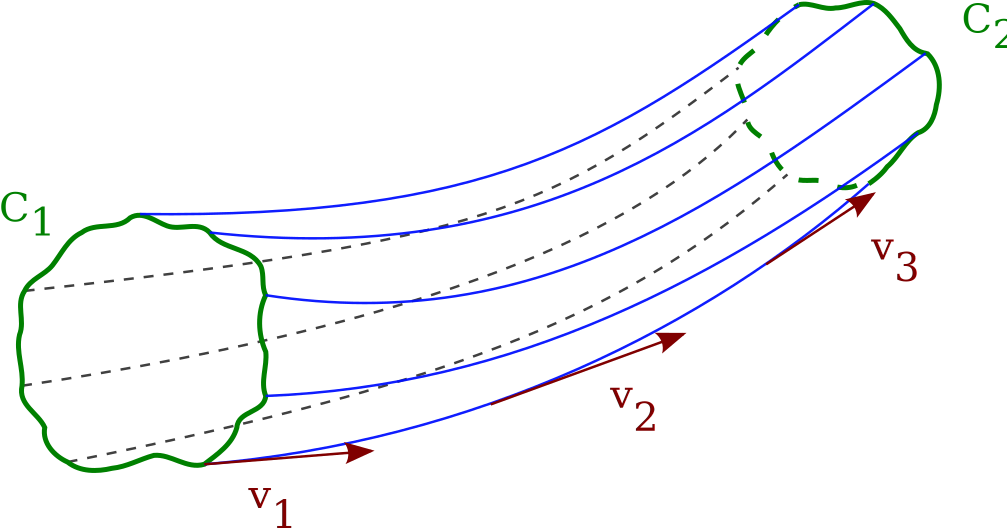
\includegraphics[width=0.8\textwidth]{img/streamtube}
\caption{Rappresentazione di un tubo di flusso e delle sue linee di flusso. In verde sono rappresentate le curve da cui ha origine il tubo di flusso e in blu le linee di flusso.} \label{fig:streamtube}
\end{center}
\end{figure}
Facendo riferimento alla figure \ref{fig:streamtube} definiamo il \textit{tubo di flusso} come lo spazio individuato dalla superficie tubolare che si forma tracciando una linea di flusso passante per ogni punto di una curva chiusa che non sia essa stessa una linea di flusso. Tale superficie tubolare non verrà mai attraversata in nessun punto dal fluido nell'istante considerato. Quindi in base al fluire del flusso (descritto dalle linee di flusso), alla curva chiusa $C1$ scelta al tempo iniziale $t=0$ e al tempo finale $t$ si ottiene un certo tubo di flusso. Ci chiediamo ora come varia la circuitazione \ref{eq:Viscosità8} dal tempo iniziale al tempo finale, cioè tra le due sezioni del tubo di flusso. Questa variazione è data dal \textit{teorema di Kelvin}
\begin{EQ}
\begin{equation}
\der{\Gamma}{t} = \Gamma (t) = \int_S \scal{\omega}{}\dd \V{S} = \int_S \quadre{\derP{\V{\omega}}{t}-\Rot{}(\vett{u}{\omega})}\cdot \dd \V{S} = 0
\end{equation}
\end{EQ}
dove l'ultima uguaglianza vale nel caso inviscido, il quale implica appunto che il termine tra le parentesi quadre sia nullo (\ref{eq:Viscosità9}). Il teorema di Kelvin per un fluido inviscido afferma quindi che la circuitazione della velocità fluida si conserva lungo i tubi di flusso. Questo risultato può essere interpretato come una conservazione del momento angolare: infatti poichè la circuitazione è la stessa lungo tutti i bordi delle sezioni di un tubo di flusso, si ha che se il tubo si restringe (o si allarga) la velocità lungo la curva chiusa deve aumentare (o diminuire). Se quindi la lunghezza del circuito aumenta la rotazione del fluido diminuisce, viceversa aumenta se la lunghezza del circuito diminuisce. Un altro modo per interpretare questo risultato consiste nel considerare il volume del tubo di flusso. Esso è racchiuso dalle superfici delimitate dai circuiti $C1$ e $C2$, e dalla superficie laterale data dalle linee di flusso che congiungono ciascun punto di $C1$ con uno e un solo punto di $C2$\footnote{Le linee di flusso non si incrociano mai, quindi per come è definito un tubo di flusso, i punti di $C1$ e di $C2$ sono collegati biunivocamente da una sola linea di flusso.}. Il teorema di Kelvin dice che il flusso di $\omega$ attraverso $S1$ è lo stesso attraverso $S2$. Essendo $\omega$ definito come un rotore, la sua divergenza è nulla. Quindi l'integrale di volume della divergenza di $\omega$ è nullo, ma per il teorema della divergenza tale integrale è uguale al flusso di $\omega$ attraverso la superficie del volume considerato. Ma poichè il flusso attravero $S1$ è uguale e opposto al flusso attraverso $S2$ (per il teorema di Kelvin), si ha che il flusso della vorticità attraverso la superficie laterale del tubo di flusso è nullo. Questo significa che le linee di vorticità sono legate alle linee di flusso; quando le linee di flusso si allargano si modificano di conseguenza le linee di vorticità, che restano tangenti alle linee di flusso della superficie laterale del tubo. Ciascuna linea di vorticità connette tra loro elementi fluidi associati a diverse linee di flusso\footnote{Tornando all'analogo del campo magnetico, si ha che per un fluido con resistività nulla vale il teorema di Kelvin.}.

Dimostriamo ora il teorema di Kelvin. Abbiamo che la circuitazione dipende dal tempo attraverso la velocità $\V{u}$ e il circuito $C$. Pertanto 
\begin{equation}
\der{\Gamma}{t} = \oint_C \derL{\V{u}}{t} \cdot \dd \V{l} + \oint_C \scal{u}{} \derL{}{t} \dd \V{l} \label{eq:Viscosità10}
\end{equation}
e iniziamo calcolando il primo integrale. Indichiamo con $\V{A}(t)$ e $\V{B}(t)$ i vettori che indicano rispettivamente il punto iniziale e finale dell'elemento di curva $\dd \V{l}$ al tempo $t$. Lasciando evolvere il sistema fino al tempo $t+\delta t$, i vettori $\V{A}$ e $\V{B}$ evolvono seguendo le linee di flusso; il nuovo elemento di curva sarà $\dd \V{l}(t+\delta t)$ delimitato dai vettori $\V{A}(t+\delta t)$ e $\V{B}(t+\delta t)$, collegati con rispettivi vettori al tempo $t$ rispettivamente da $\V{u}(\V{A)}\delta t$ e $\V{u}(\V{B})\delta t$. Pertanto vale
\begin{equation}
\dd \V{l} (t+\delta t) = \V{B}(t+\delta t)-\V{A}(t+\delta t) = \V{B}(t) + \V{u}(\V{B})\delta t - \V{A}(t) - \V{u}(\V{A})\delta t = \dd \V{l}(t) + (\dd \scal{l}{\nabla})\V{u} \delta t
\end{equation}
Possiamo così stimare la derivata lagrangiana nell'integranda del secondo integrale
\begin{equation}
\derL{}{t} \dd \V{l} = \dfrac{\dd \V{l} (t+\delta t) - \dd \V{l} (t)}{\delta t} = (\dd \scal{l}{\nabla})\V{u}
\end{equation}
L'integranda può quindi essere riscritta come
\begin{equation}
\scal{u}{} \derL{}{t} \dd \V{l} = \scal{u}{}(\dd \scal{l}{\nabla})\V{u} = \Grad\tonde{\inv{2}u^2}\cdot\dd \V{l}
\end{equation}
Segue che il secondo integrale è la circuitazione di un gradiente, la quale è nulla. Pertanto il secondo integrale è nullo, e quindi abbiamo ottenuto il risultato generale che la derivata temporale della circuitazione di un campo di vettoriale è data solo dai contributi delle variazioni temporali del campo vettoriale, mentre non si hanno contributi dovuti alla variazione temporali del circuito. Calcoliamo ora il primo integrale: ricordiamo che, sfruttando la relazione \ref{eq:Viscosità11} la derivata lagrangiana della velocità è
\begin{equation}
\derL{\V{u}}{t} = \derP{\V{u}}{t} + \Grad\tonde{\dfrac{u^2}{s}} - \vett{u}{\omega}
\end{equation}
Anche in questo caso il termine con il gradiente ha circuitazione nulla, pertanto
\begin{equation}
\der{\Gamma}{t} = \oint_C \derL{\V{u}}{t} \cdot \dd \V{l} = \oint_C \quadre{\der{\V{u}}{t} - \vett{u}{\omega}}\cdot \dd \V{l} = \int_S \quadre{\derP{\V{\omega}}{t}-\Rot{}(\vett{u}{\omega})}\cdot \dd \V{S}
\end{equation}
Abbiamo così dimostrato il teorema. Esso esprime quanto già avevamo considerato dall'equazione di Helmholtz \ref{eq:Viscosità12}, ovvero che se il fluido inizialmente privo di vortici ha viscosità nulla, allora è impossibile generare dei vortici. Infatti se la viscosità è nulla, il teorema di Kelvin implica che la ciscuitazione non varia nel tempo, e che quindi il flusso della vorticità si deve conservare. Pertanto se la vorticità è inizialmente nulla, è nulla anche al tempo $t$.

Ora che abbiamo definito la quantità associata alla turbolenza, ovvero la volrticità, e specificato le sue principali caratteristiche con il teorema di Kelvin, possiamo discutere a livello quantitativo la turbolenza. Distinguiamo i \textit{fluidi laminari}, in cui non sono presenti vortici, e \textit{fluidi turbolenti} in cui invece sono presenti. La descrizione della vorticità è molto complicata; seguiremo l'approccio adottato da Kolmogorov per i moti vorticosi nei fluidi incomprimibili. I vortici si formano su grandi scale, trasportando una certa energia; dopodichè si scompongono progressivamente in vortici più piccoli che trasportano frazioni dell'energia totale del vortice iniziale. Infine quando i vortici raggiungono le piccole scale in cui la viscosità diventa rilevante, scompaiono dissipando la loro energia nel fluido. Questi processi sono quantificati da due termini nell'equazione di Navier-Stokes \ref{eq:Viscosità6}: il termine non lineare $(\scal{u}{\nabla})\V{u}$ genera i moti caotici turbolenti, mentre il termine viscoso $\nu\Grad^2 \V{u}$ è responsabile della dissipazione dei vortici (ma anche della generazione; infatti per quanto visto per il teorema di Kelvin, se la viscosità è nulla, non è possibile generare vorticità). I moti vorticosi verranno dissipati quando il termine dissipativo diventa dello stesso ordine di grandezza del termine non lineare. Per determinare quando ciò avviene possiamo adottare un'analisi dimensionale dei due termini per ricavare le scale di lunghezza tipiche a cui avvengono la dissipazione e la generazione dei vortici. Consideriamo in generale la scala di lunghezze $\lambda$, e supponiamo che su tale scala la velocità fluida sia $u_\lambda$. Il termine non lineare è esprimibile come
\begin{equation}
(\scal{u}{\nabla})\V{u} \,\,\,\,\,\,\,\,\,\,\,\,\,\,\, \Longrightarrow \,\,\,\,\,\,\,\,\,\,\,\,\,\,\,\dfrac{u_\lambda^2}{\lambda} \label{eq:Viscosità13}
\end{equation}
mentre il termine dissipativo può essere scritto come
\begin{equation}
\nu \Grad^2 \V{u} \,\,\,\,\,\,\,\,\,\,\,\,\,\,\, \Longrightarrow \,\,\,\,\,\,\,\,\,\,\,\,\,\,\,\nu \dfrac{u_\lambda}{\lambda^2} \label{eq:Viscosità14}
\end{equation}
Il rapporto tra questi due termini è 
\begin{EQ}
\begin{equation}
Re \equiv \dfrac{u_\lambda \lambda}{\nu}
\end{equation}
\end{EQ}
è un numero adimensionale che indica quanto conta il termine non lineare dell'equazione di Navier-Stokes, rispetto al termine viscoso. Questo rapporto è noto come \textit{numero di Reynolds}\footnote{Fisicamente il numero di Reynolds rappresenta il rapporto tra le forze di inerzia e quelle viscose agenti su un elemento fluido in moto con velocità $\V{u}$.}. Dagli studi sperimentali si osserva che la turbolenza si genera tipicamente per $Re>10^3 - 10^4$. Tali valori variano a seconda dei fluidi. Vediamo quindi che la turbolenza si genera per basse viscosità, infatti se abbiamo un fluido molto viscoso, come ad esempio la lava, non si genera turbolenza e il fluido resta a regime laminare. Inoltre dalle diverse dipendenze dalla velocità e dalla scala di lunghezza del termine non lineare e del termine viscoso (equazioni \ref{eq:Viscosità13} e \ref{eq:Viscosità14}), si osserva che la dissipazione domina su piccole scale, mentre su grandi scale domina la generazione di turbolenza, la quale domina anche per grandi velocità.  

La scala a cui si ha dissipazione della vorticosità è ottenuta fissando il numero di Reynolds a uno. Tale scala è 
\begin{equation}
\lambda_K = \dfrac{\nu}{u_K} \label{eq:Viscosità16}
\end{equation}

Come abbiamo già accennato, l'approccio di Kolmogorov\footnote{L'intuizione di Kolmogorov è stata quella di capire che il comportamento della turbolenza, nelle suddette condizioni, dipende esclusivamente da $\varepsilon$ (energia dissipata, o equivalentemente iniettata, per unità di tempo e di massa) e da $\nu$ (viscosità).} assume turbolenza stazionaria, ovvero si ipotizza che la densità energetica nei moti vorticosi è costante nel tempo. Ciò significa che l'energia dissipata dalla viscosità viene compensata da un'altro processo che inietta energia nel sistema, mantenendo la turbolenza. In altri termini il flusso di energia da scale maggiori a scale minori deve essere costante. Chiamiamo $\varepsilon$ l'energia dissipata per unità di tempo e massa.
Ricordando l'equazione \ref{eq:Viscosità15}, abbiamo che il tasso di dissipazione $D$ per unità di volume è \footnote{Sfruttiamo il fatto che dimensionalmente il tensore delle deformazioni ha le dimensioni di una velocità su una lunghezza.}
\begin{equation}
D \sim \eta e_{ij}^2 \sim \nu\rho \dfrac{u_K^2}{\lambda_K^2} \equiv \rho \label{eq:Viscosità17}
\end{equation}
Da questa equazione, e usando la \ref{eq:Viscosità16} possiamo ottenere un'espressione per $\varepsilon$, ovvero
\begin{EQ}
\begin{equation}
\varepsilon = \dfrac{\nu^3}{\lambda_K^4} \label{eq:Viscosità18}
\end{equation}
\end{EQ}
Sottolienaimo che le condizioni \ref{eq:Viscosità16} e \ref{eq:Viscosità17} derivano rispettivamenta dall'ipotesi che alla scala di Kolmogorv il numero di Reynolds è dell'ordine dell'unità e dalla stazionarietà della turbolenza.
Da questa relazione otteniamo che la scala di Kolmogorov e la velocità di Kolmogorov (ovvero le quantità che descrivono la vorticosità) dipendono unicamente dalla voscosità e dall'energia per unità di tempo e massa iniettata nel sistema (la quale coincide con quella dissipata per l'ipotesi di stazionarietà, che rende possibile usare $\varepsilon$ per indicarle entrambe).
\begin{EQ}
\begin{align}
&\lambda_K = \tonde{\dfrac{\nu^3}{\varepsilon}}^{1/4}
&u_K = (\nu \varepsilon)^{1/4}
\end{align}
\end{EQ}
Resta ora da trovare il legame tra le grandi scale di distanza $L$ e di velocità $u_L$ a cui avviene l'iniezione di energia con le piccole scale di Kolmogorov. Per farlo procediamo da una pura analisi dimensionale. Abbiamo definito $\varepsilon$ come l'energia iniettata/dissipata per unità di tempo e massa. Essa sarà quindi esprimibile dal quadrato della velocità alla scala $L$ (che ha le dimensioni di un'energia per unità di massa) diviso il tempo scala dell'iniezione, dato dal rapporto tra la scala $L$ e la velocità di scala $u_L$. Otteniamo così
\begin{equation}
\epsilon = \dfrac{u_L^3}{L}
\end{equation}
Eguagliando quest'ultima equazione con la \ref{eq:Viscosità18} si ottiene facilmente 
\begin{equation}
\dfrac{L}{\lambda_K} = \mathit{Re}^{3/4}
\end{equation}
dove abbiamo identificato $\mathit{Re} = u_L L/\nu$ con il numero di Reynolds alla scala di iniezione, il quale è per definizione molto maggiore di uno, poichè le turbolenze si innescano solo per numeri di Reynolds elevati. Quanto più grande è il numero di Reynolds, tanto più grande è il divario tra la scala di iniezione e quella di Kolmogorov a cui diventa rilevante la disipazione.

Un ultimo contributo fornito da Kolmogorov è dato dallo studio dello \textit{spettro di Kolmogorov} ovvero da come l'energia è distribuita sulle diverse scale di lunghezza. Essendo uno spettro di Fourier la dipendenza dell'energia dalle lunghezze è tramite i numeri d'onda $\V{k}$. 
\begin{figure}
\begin{center}
\includegraphics[width=0.8\textwidth]{img/Kolmogorov}
\caption{Spettro di Kolmogorov}\label{fig:Kolmogorov}
\end{center}
\end{figure}
Per determinare lo spettro si aggiunge l'ipotesi di turbolenza isotropa, il che implica una dipendenza dell'energia dal solo modulo del numero d'onda $k$. Il fatto che i fenomeni vorticosi avvengono a partire dalle scale $L$ di iniezione dell'energia, fino alle scale $\lambda_K$ di dissipazione dell'energia, implica che fuori da questo intervallo l'energia decresce rapidamente a zero. Inoltre nel regime intermedio, detto \textit{regime inerziale}, l'energia dipende solamente dall'energia per unità di tempo e di massa iniettata nel sistema, e dal numero d'onda (ovvero dalla scala di lunghezze) associato ai vortici, e quindi si assume che la dipendenza dell'energia da queste due quantità sia una legge di potenza\footnote{In questo regime non vi può essere dipendenza dello spettro se non dall'energia immessa nel fluido su grandi scale $\epsilon$ che genera la turbolenza, e dal numero d'onda associato ad un certo vortice. Ad esempio una dipendenza dalla viscosità del fluido è esclusa poichè in tale regime il fluido non ha ancora raggiunto scale sufficientemente piccole affinche si manifestino fenomeni di dissipazione viscosa (è come se non ci fosse viscosità).}.
Facendo riferimento all'immagine \ref{fig:Kolmogorov}, vediamo che facendo queste assunzioni, il grafico logaritmico dello spettro è una retta nel regime inerziale. Per trovare la pendenza della retta basta una semplice analisi dimensionale.
\begin{equation}
E_k \propto \varepsilon^a k^b
\end{equation}
Essendo $E_k$ un'energia per unità di massa e numero d'onda, ha le dimensioni di $L^3\, T^{-2}$. Ricordando che $\varepsilon$ ha le dimensioni di $L^2 \,T^{-3}$, si ricava banalmente
\begin{EQ}
\begin{align}
E_k \propto \varepsilon^{2/3}\,k^{-5/3}
\end{align}
\end{EQ}
La caratteristica fondamentale dello spettro di Kolmogorov nel regime inerziale è la dipendenza da $k^{-5/3}$.

In astrofisica si osservano fenomeni di turbolenze nel mezzo interstellare e intergalattico, nei dischi di accrescimento, o nelle nubi molecolari durante la formazione stellare.

\section{Accrescimento}
Concludiamo questo capitolo con dei brevi cenni ai fenomeni di accrescimento senza entrare troppo nel dettaglio, in quanto argomenti del corso di Fisica Cosmica 2.

L'obbiettivo è studiare il flusso di materia verso/da un oggetto sferico centrale. Grazie a questa simmetria scriviamo le equazioni fluide in simmetria sferica, considerando la velocità del fluido nella sola direzione radiale, ovvero $V{u}=u\vers{r}$. L'equazione di continuità diventa
\begin{equation}
\derP{\rho}{t} + \inv{r^2} \derP{}{r}\tonde{r^2 u \rho}=0
\end{equation}
In condizioni stazionarie ($\dpt\rho=0$) risulta che $\rho u r^2$ è una costante, e quindi è una costante anche la quantità
\begin{equation}
\dot{M} = 4\pi \rho u r^2
\end{equation}
che non è altro che massa di fluido che transita nell'unità di tempo attraverso il guscio sferico di raggio $r$; indica la variazione temporale della massa dell'oggetto centrale. L'equazione di Eulero in coordinate sferiche è invece
\begin{equation}
\derP{u}{t} + u\derP{u}{r}= -\inv{\rho}\der{p}{r} - \dfrac{GM}{r^2}  \label{eq:Accrescimento3}
\end{equation}
dove al secondo membro abbiamo tenuto conto del fatto che è presento un campo di gravità dovuto all'oggetto centrale di massa $M$. Aggiungendo l'ipotesi di stazionarietà risulta che il primo membro può essere riscritto semplicemente come $u\der{u}{r}$. Sfruttando la relazione 
\begin{equation}
\der{p}{r}=\sound^2 \der{\rho}{r}
\end{equation}
riscriviamo l'equazione di Eulero come
\begin{equation}
u^2\der{(\ln u)}{r} = -\sound^2 \der{(\ln\rho)}{r} - \dfrac{GM}{r^2} \label{eq:Accrescimento1}
\end{equation}
Sappiamo inoltre che $\dot{M}$ è una costante, e quindi anche il suo logaritmo è una costante, che significa che la sua derivata rispetto a $r$ è nulla, ovvero
\begin{equation}
\der{(\ln \dot{M})}{r} = \der{(\ln\rho)}{r} + \der{(\ln u)}{r} + \dfrac{2}{r} = 0
\end{equation}
da cui si ottiene
\begin{equation}
-\der{(\ln\rho)}{r} = \der{(\ln u)}{r} + \dfrac{2}{r} 
\end{equation}
Sostituendo questo termine nella \ref{eq:Accrescimento1} si ottiene
\begin{equation}
\sound^2 \der{(\ln u)}{r} + \dfrac{2\sound^2}{r}  - \dfrac{GM}{r^2} = u^2\der{(\ln u)}{r}
\end{equation}
che può essere riscritta più convenientemente nella seguente forma
\begin{EQ}
\begin{equation}
(u^2-\sound^2) \der{(\ln u)}{r} = \dfrac{2\sound^2}{r} \tonde{1-\dfrac{GM}{2\sound^2 r}} \label{eq:Accrescimento2}
\end{equation}
\end{EQ}
Questa equazione permette di descrivere i fenomeni di accrescimento (la massa del fluido si muove verso l'oggetto centrale) e quelli di vento stellare (la massa del fluido si vuove dall'oggetto centrale). Nel caso di vento si ha velocità nulla a $r=0$ che aumenta progressivamente diventando infinita per $r\to\infty$. Viceversa nel caso di accrescimento si ha $u=0$ per raggi molto grandi e $u\to\infty$ per $r\to 0$. È chiaro che in entrambi i casi si ha un raggio a cui la velocità supera (in un senso o nell'altro) la velocità del suono. Tale raggio limite a cui si ha $u=\sound$ è detto \textit{raggio sonico} $r_\mathrm{s}$, e può essere facilmente trovato dall'equazione \ref{eq:Accrescimento2}, trovando
\begin{equation}
r_\mathrm{s} = \dfrac{GM}{2\sound^2}
\end{equation}
Ad una distanza pari al raggio sonico si ha che il membro di destra dell'equazione \ref{eq:Accrescimento2} si annulla, il che implica o che la velocità del fluido è pari a quella del suono, o che la velocità ha raggiunto un massimo.

Il tasso di accrescimento al raggio sonico vale
\begin{equation}
\dot{M} = 4\pi \dfrac{G^2M^2}{4\sound^4} \rho_\mathrm{s} \sound = \dfrac{\pi G^2 M^2}{\sound^3(r_\mathrm{s})} \label{eq:Accrescimento7}
\end{equation}
dove con $\sound(r_\mathrm{s})$ indichiamo il fatto che la velocità del suono è associata al raggio sonico, poichè in generale è funzione di $r$. Quello che si vuole fare ora è riuscire a dare una stima del tasso di accrescimento da quantità valutate a grandi distanze dall'oggetto centrale (le quali sono pù facili da misurare). Cerchiamo quindi di riscrivere questa stima in termini di tali quantità. 
Iniziamo supponendo che l'equazione di stato sia politropica $p = k\rho^\gamma$ con $k$ costante di proporzionalità. Si può scrivere
\begin{equation}
\inv{\rho}\der{p}{r} = \gamma k \rho^{\gamma-2}\der{\rho}{r} = \dfrac{\gamma}{\gamma-1}k \der{}{r}(\rho^{\gamma-1})
\end{equation}
Sostituendo quest'equazione nella \ref{eq:Accrescimento3}\footnote{Il termine $\derP{u}{t}=0$ poichè stiamo considerando il caso stazionario.} e integrando rispetto a $r$ si ottiene 
\begin{equation}
\inv{2}u^2+\dfrac{\sound^2}{\gamma-1}-\dfrac{GM}{r} = cost \label{eq:Accrescimento4}
\end{equation}
Quest'equazione è una forma dell'equazione di Bernoulli \ref{eq:Bernoulli}. Fino ad ora la trattazione è valida sia per il caso di accrescimento che di vento. Concentriamoci sul primo caso, in cui si ha che $u=0$ per $r\to\infty$. Quest'ipotesi consente di stimare dalla \ref{eq:Accrescimento4} la costante di Bernoulli a $\dfrac{c_\infty^2}{\gamma-1}$, dove con $c_\infty$ intendiamo la velocità del suono all'infinito. Valutando la \ref{eq:Accrescimento4} al raggio sonico, otteniamo la relazione
\begin{equation}
\sound^2(r_\mathrm{s}) = \dfrac{2}{5-3\gamma}c_\infty^2 \label{eq:Accrescimento5}
\end{equation}
Infine, considernado che $\sound^2\propto\rho^{\gamma-1}$ risulta
\begin{equation}
\tonde{\dfrac{c_\infty}{\sound(r_\mathrm{s})}} = \tonde{\dfrac{\rho_\infty}{\rho_s}}
\end{equation}
da cui otteniamo
\begin{equation}
\rho_s = \rho_\infty \tonde{\dfrac{2}{5-3\gamma}}^{1/(\gamma-1)} \label{eq:Accrescimento6}
\end{equation}
A questo punto, sostituendo le \ref{eq:Accrescimento5} e \ref{eq:Accrescimento6} nella \ref{eq:Accrescimento7}, otteniamo
\begin{EQ}
\begin{equation}
\dot{M} = \pi \dfrac{(GM)^2}{c_\infty} \rho_\infty\quadre{\dfrac{2}{5-3\gamma}}^{\dfrac{5-3\gamma}{2(\gamma-1)}}
\end{equation}
\end{EQ}
Questo tasso di accrescimento è noto come \textit{accrescimento di Bondi}.
Questo risultato non va bene per $\gamma\geq 5/3$: in queste condizioni il gas è troppo poco comprimibile per raggiungere velocità soniche. In questa derivazione abbiamo considerato un fluido in accrescimento su di un oggetto centrale in quiete (rispetto al fluido). Un'altra configurazione possibile è quella di un oggetto, ad esempio una stella, in moto all'interno di un fluido con velocità $v_\infty$. In questo caso il tasso di accrescimento è
\begin{equation}
\dot{M} = 4\pi \dfrac{(GM)^2}{v_\infty^3}\rho_\infty
\end{equation}
detto \textit{accrescimento di Hoyle-Lyttleton}. In questo caso il moto dell'oggetto nel fluido domina sugli effetti di pressione ($\sound\ll v_\infty$). Il caso più generale è quello che considera entrambi gli effetti: in tal caso il tasso di accrescimento è
\begin{equation}
\dot{M} = 4\pi \dfrac{(GM)^2}{v_\infty^3 + c_\infty^3}\rho_\infty
\end{equation}
detto \textit{accrescimento di Bondi-Hoyle}.

Notiamo infine che in questa discussione abbiamo fatto un'ipotesi molto vincolante, ovvero la simmetria sferica. Nella quasi totalita dei casi i sistemi in accresciemento sono in rotazione. Questo implica che a grandi distanze il sistema è in buona approssimazione sferico, ma avvicinandosi all'oggetto centrale, la conservazione del momento angolare implica uno schiacciamento del sistema, per cui l'accrescimento avviene prevalentemente nel piano di rotazione del sistema. Il risultato qui ottenuto è una prima approssimazione del problema dell'accrescimento, ma che fallisce nella descrizione più dettagliata dei sistemi come i dischi di accrescimento, trattati nel secondo modulo di questo corso.



\backmatter					% è la parte finale del documento
\addcontentsline{toc}{chapter}{Bibliografia}
\nocite{*}
\bibliography{biblio}

\end{document}